\documentclass[twoside]{book}

% Packages required by doxygen
\usepackage{fixltx2e}
\usepackage{calc}
\usepackage{doxygen}
\usepackage[export]{adjustbox} % also loads graphicx
\usepackage{graphicx}
\usepackage[utf8]{inputenc}
\usepackage{makeidx}
\usepackage{multicol}
\usepackage{multirow}
\PassOptionsToPackage{warn}{textcomp}
\usepackage{textcomp}
\usepackage[nointegrals]{wasysym}
\usepackage[table]{xcolor}

% Font selection
\usepackage[T1]{fontenc}
\usepackage[scaled=.90]{helvet}
\usepackage{courier}
\usepackage{amssymb}
\usepackage{sectsty}
\renewcommand{\familydefault}{\sfdefault}
\allsectionsfont{%
  \fontseries{bc}\selectfont%
  \color{darkgray}%
}
\renewcommand{\DoxyLabelFont}{%
  \fontseries{bc}\selectfont%
  \color{darkgray}%
}
\newcommand{\+}{\discretionary{\mbox{\scriptsize$\hookleftarrow$}}{}{}}

% Page & text layout
\usepackage{geometry}
\geometry{%
  a4paper,%
  top=2.5cm,%
  bottom=2.5cm,%
  left=2.5cm,%
  right=2.5cm%
}
\tolerance=750
\hfuzz=15pt
\hbadness=750
\setlength{\emergencystretch}{15pt}
\setlength{\parindent}{0cm}
\setlength{\parskip}{3ex plus 2ex minus 2ex}
\makeatletter
\renewcommand{\paragraph}{%
  \@startsection{paragraph}{4}{0ex}{-1.0ex}{1.0ex}{%
    \normalfont\normalsize\bfseries\SS@parafont%
  }%
}
\renewcommand{\subparagraph}{%
  \@startsection{subparagraph}{5}{0ex}{-1.0ex}{1.0ex}{%
    \normalfont\normalsize\bfseries\SS@subparafont%
  }%
}
\makeatother

% Headers & footers
\usepackage{fancyhdr}
\pagestyle{fancyplain}
\fancyhead[LE]{\fancyplain{}{\bfseries\thepage}}
\fancyhead[CE]{\fancyplain{}{}}
\fancyhead[RE]{\fancyplain{}{\bfseries\leftmark}}
\fancyhead[LO]{\fancyplain{}{\bfseries\rightmark}}
\fancyhead[CO]{\fancyplain{}{}}
\fancyhead[RO]{\fancyplain{}{\bfseries\thepage}}
\fancyfoot[LE]{\fancyplain{}{}}
\fancyfoot[CE]{\fancyplain{}{}}
\fancyfoot[RE]{\fancyplain{}{\bfseries\scriptsize Generated by Doxygen }}
\fancyfoot[LO]{\fancyplain{}{\bfseries\scriptsize Generated by Doxygen }}
\fancyfoot[CO]{\fancyplain{}{}}
\fancyfoot[RO]{\fancyplain{}{}}
\renewcommand{\footrulewidth}{0.4pt}
\renewcommand{\chaptermark}[1]{%
  \markboth{#1}{}%
}
\renewcommand{\sectionmark}[1]{%
  \markright{\thesection\ #1}%
}

% Indices & bibliography
\usepackage{natbib}
\usepackage[titles]{tocloft}
\setcounter{tocdepth}{3}
\setcounter{secnumdepth}{5}
\makeindex

% Hyperlinks (required, but should be loaded last)
\usepackage{ifpdf}
\ifpdf
  \usepackage[pdftex,pagebackref=true]{hyperref}
\else
  \usepackage[ps2pdf,pagebackref=true]{hyperref}
\fi
\hypersetup{%
  colorlinks=true,%
  linkcolor=blue,%
  citecolor=blue,%
  unicode%
}

% Custom commands
\newcommand{\clearemptydoublepage}{%
  \newpage{\pagestyle{empty}\cleardoublepage}%
}

\usepackage{caption}
\captionsetup{labelsep=space,justification=centering,font={bf},singlelinecheck=off,skip=4pt,position=top}

%===== C O N T E N T S =====

\begin{document}

% Titlepage & ToC
\hypersetup{pageanchor=false,
             bookmarksnumbered=true,
             pdfencoding=unicode
            }
\pagenumbering{roman}
\begin{titlepage}
\vspace*{7cm}
\begin{center}%
{\Large Staci }\\
\vspace*{1cm}
{\large Generated by Doxygen 1.8.11}\\
\end{center}
\end{titlepage}
\clearemptydoublepage
\tableofcontents
\clearemptydoublepage
\pagenumbering{arabic}
\hypersetup{pageanchor=true}

%--- Begin generated contents ---
\chapter{staci}
\label{md_README}
\hypertarget{md_README}{}
\input{md_README}
\chapter{Hierarchical Index}
\section{Class Hierarchy}
This inheritance list is sorted roughly, but not completely, alphabetically\+:\begin{DoxyCompactList}
\item \contentsline{section}{Agelem}{\pageref{class_agelem}}{}
\begin{DoxyCompactList}
\item \contentsline{section}{Buko\+Mutargy}{\pageref{class_buko_mutargy}}{}
\item \contentsline{section}{Csatorna}{\pageref{class_csatorna}}{}
\item \contentsline{section}{Cso}{\pageref{class_cso}}{}
\item \contentsline{section}{Jelleggorbes\+Fojtas}{\pageref{class_jelleggorbes_fojtas}}{}
\item \contentsline{section}{Konst\+Nyomas}{\pageref{class_konst_nyomas}}{}
\item \contentsline{section}{Szivattyu}{\pageref{class_szivattyu}}{}
\item \contentsline{section}{Vegakna}{\pageref{class_vegakna}}{}
\item \contentsline{section}{Visszacsapo\+Szelep}{\pageref{class_visszacsapo_szelep}}{}
\end{DoxyCompactList}
\item \contentsline{section}{A\+L\+L\+X\+M\+L\+Clear\+Tag}{\pageref{struct_a_l_l_x_m_l_clear_tag}}{}
\item \contentsline{section}{Any\+Option}{\pageref{class_any_option}}{}
\item \contentsline{section}{arithcode}{\pageref{classarithcode}}{}
\item \contentsline{section}{Csomopont}{\pageref{class_csomopont}}{}
\item \contentsline{section}{data\+\_\+io}{\pageref{classdata__io}}{}
\item \contentsline{section}{huffcode}{\pageref{classhuffcode}}{}
\item \contentsline{section}{Next\+Token}{\pageref{struct_next_token}}{}
\item \contentsline{section}{N\+R\+Mat$<$ T $>$}{\pageref{class_n_r_mat}}{}
\item \contentsline{section}{N\+R\+Mat3d$<$ T $>$}{\pageref{class_n_r_mat3d}}{}
\item \contentsline{section}{N\+R\+Vec$<$ T $>$}{\pageref{class_n_r_vec}}{}
\item \contentsline{section}{N\+R\+Vec$<$ DP $>$}{\pageref{class_n_r_vec}}{}
\item \contentsline{section}{N\+R\+Vec$<$ unsigned long $>$}{\pageref{class_n_r_vec}}{}
\item \contentsline{section}{Staci}{\pageref{class_staci}}{}
\item \contentsline{section}{Staci\+Exception}{\pageref{class_staci_exception}}{}
\item \contentsline{section}{wavefilt}{\pageref{classwavefilt}}{}
\item \contentsline{section}{X\+ML}{\pageref{struct_x_m_l}}{}
\item \contentsline{section}{X\+M\+L\+Attribute}{\pageref{struct_x_m_l_attribute}}{}
\item \contentsline{section}{X\+M\+L\+Character\+Entity}{\pageref{struct_x_m_l_character_entity}}{}
\item \contentsline{section}{X\+M\+L\+Clear}{\pageref{struct_x_m_l_clear}}{}
\item \contentsline{section}{X\+M\+L\+Node}{\pageref{struct_x_m_l_node}}{}
\item \contentsline{section}{X\+M\+L\+Node\+Contents}{\pageref{struct_x_m_l_node_contents}}{}
\item \contentsline{section}{X\+M\+L\+Parser\+Base64\+Tool}{\pageref{class_x_m_l_parser_base64_tool}}{}
\item \contentsline{section}{X\+M\+L\+Results}{\pageref{struct_x_m_l_results}}{}
\end{DoxyCompactList}

\chapter{Class Index}
\section{Class List}
Here are the classes, structs, unions and interfaces with brief descriptions\+:\begin{DoxyCompactList}
\item\contentsline{section}{\hyperlink{class_agelem}{Agelem} }{\pageref{class_agelem}}{}
\item\contentsline{section}{\hyperlink{struct_a_l_l_x_m_l_clear_tag}{A\+L\+L\+X\+M\+L\+Clear\+Tag} }{\pageref{struct_a_l_l_x_m_l_clear_tag}}{}
\item\contentsline{section}{\hyperlink{class_any_option}{Any\+Option} }{\pageref{class_any_option}}{}
\item\contentsline{section}{\hyperlink{classarithcode}{arithcode} }{\pageref{classarithcode}}{}
\item\contentsline{section}{\hyperlink{class_buko_mutargy}{Buko\+Mutargy} }{\pageref{class_buko_mutargy}}{}
\item\contentsline{section}{\hyperlink{class_csatorna}{Csatorna} }{\pageref{class_csatorna}}{}
\item\contentsline{section}{\hyperlink{class_cso}{Cso} }{\pageref{class_cso}}{}
\item\contentsline{section}{\hyperlink{class_csomopont}{Csomopont} }{\pageref{class_csomopont}}{}
\item\contentsline{section}{\hyperlink{classdata__io}{data\+\_\+io} }{\pageref{classdata__io}}{}
\item\contentsline{section}{\hyperlink{classhuffcode}{huffcode} }{\pageref{classhuffcode}}{}
\item\contentsline{section}{\hyperlink{class_jelleggorbes_fojtas}{Jelleggorbes\+Fojtas} }{\pageref{class_jelleggorbes_fojtas}}{}
\item\contentsline{section}{\hyperlink{class_konst_nyomas}{Konst\+Nyomas} }{\pageref{class_konst_nyomas}}{}
\item\contentsline{section}{\hyperlink{struct_next_token}{Next\+Token} }{\pageref{struct_next_token}}{}
\item\contentsline{section}{\hyperlink{class_n_r_mat}{N\+R\+Mat$<$ T $>$} }{\pageref{class_n_r_mat}}{}
\item\contentsline{section}{\hyperlink{class_n_r_mat3d}{N\+R\+Mat3d$<$ T $>$} }{\pageref{class_n_r_mat3d}}{}
\item\contentsline{section}{\hyperlink{class_n_r_vec}{N\+R\+Vec$<$ T $>$} }{\pageref{class_n_r_vec}}{}
\item\contentsline{section}{\hyperlink{class_staci}{Staci} }{\pageref{class_staci}}{}
\item\contentsline{section}{\hyperlink{class_staci_exception}{Staci\+Exception} }{\pageref{class_staci_exception}}{}
\item\contentsline{section}{\hyperlink{class_szivattyu}{Szivattyu} }{\pageref{class_szivattyu}}{}
\item\contentsline{section}{\hyperlink{class_vegakna}{Vegakna} }{\pageref{class_vegakna}}{}
\item\contentsline{section}{\hyperlink{class_visszacsapo_szelep}{Visszacsapo\+Szelep} }{\pageref{class_visszacsapo_szelep}}{}
\item\contentsline{section}{\hyperlink{classwavefilt}{wavefilt} }{\pageref{classwavefilt}}{}
\item\contentsline{section}{\hyperlink{struct_x_m_l}{X\+ML} }{\pageref{struct_x_m_l}}{}
\item\contentsline{section}{\hyperlink{struct_x_m_l_attribute}{X\+M\+L\+Attribute} }{\pageref{struct_x_m_l_attribute}}{}
\item\contentsline{section}{\hyperlink{struct_x_m_l_character_entity}{X\+M\+L\+Character\+Entity} }{\pageref{struct_x_m_l_character_entity}}{}
\item\contentsline{section}{\hyperlink{struct_x_m_l_clear}{X\+M\+L\+Clear} }{\pageref{struct_x_m_l_clear}}{}
\item\contentsline{section}{\hyperlink{struct_x_m_l_node}{X\+M\+L\+Node} }{\pageref{struct_x_m_l_node}}{}
\item\contentsline{section}{\hyperlink{struct_x_m_l_node_contents}{X\+M\+L\+Node\+Contents} }{\pageref{struct_x_m_l_node_contents}}{}
\item\contentsline{section}{\hyperlink{class_x_m_l_parser_base64_tool}{X\+M\+L\+Parser\+Base64\+Tool} }{\pageref{class_x_m_l_parser_base64_tool}}{}
\item\contentsline{section}{\hyperlink{struct_x_m_l_results}{X\+M\+L\+Results} }{\pageref{struct_x_m_l_results}}{}
\end{DoxyCompactList}

\chapter{Class Documentation}
\hypertarget{class_agelem}{}\section{Agelem Class Reference}
\label{class_agelem}\index{Agelem@{Agelem}}
Inheritance diagram for Agelem\+:\begin{figure}[H]
\begin{center}
\leavevmode
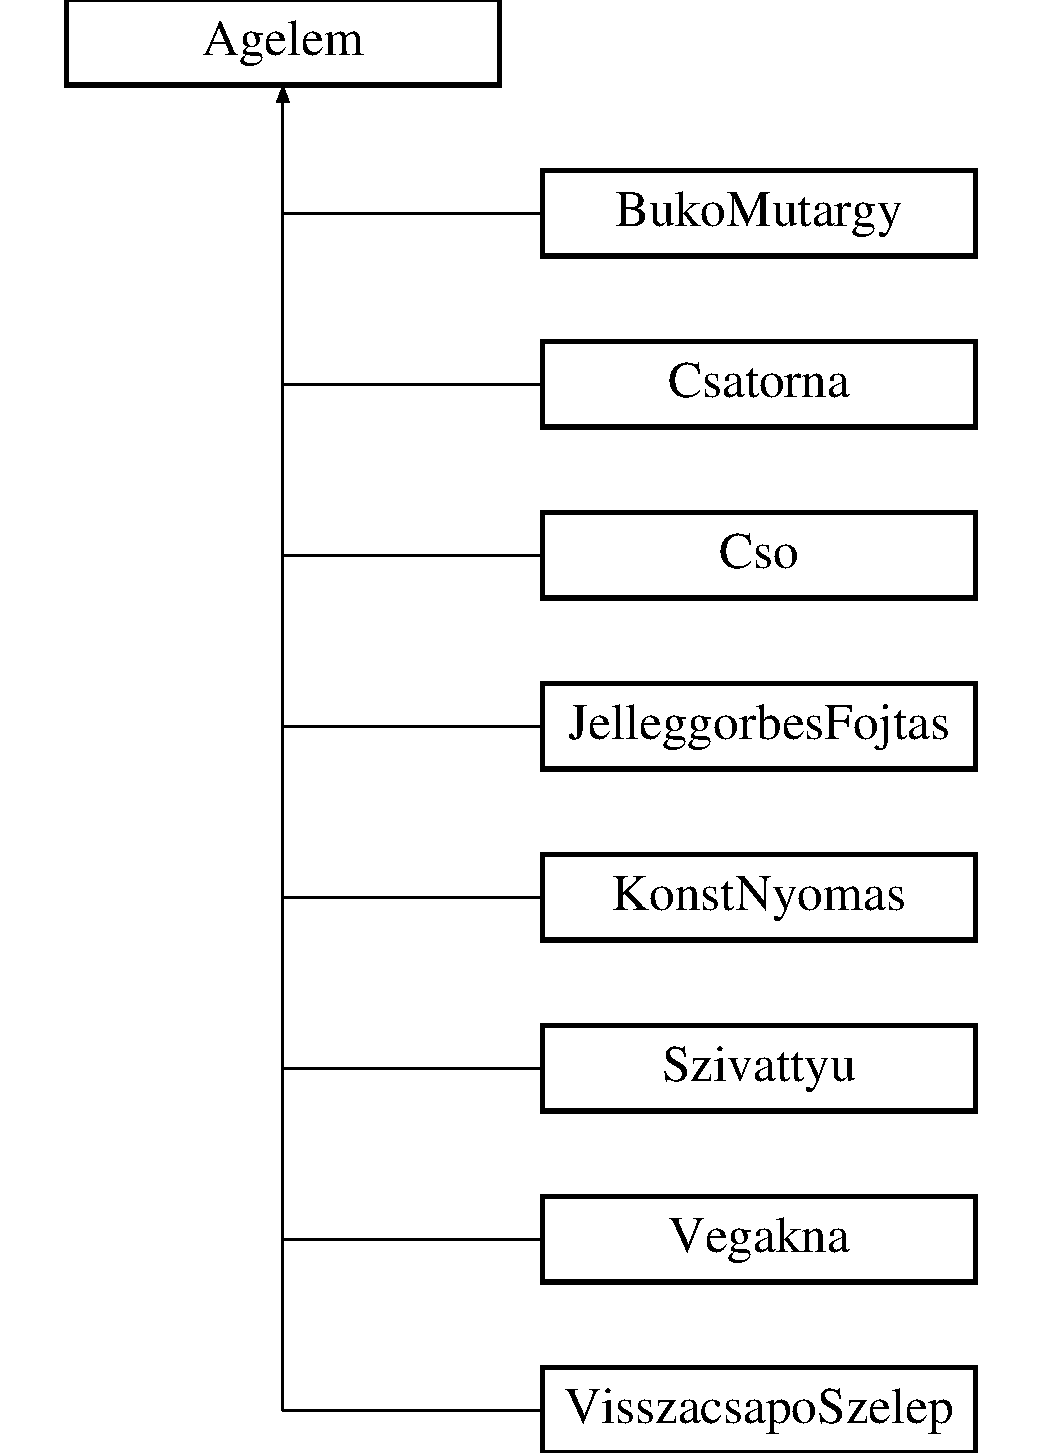
\includegraphics[height=9.000000cm]{class_agelem}
\end{center}
\end{figure}
\subsection*{Public Member Functions}
\begin{DoxyCompactItemize}
\item 
void {\bfseries logfile\+\_\+write} (string msg, int msg\+\_\+debug\+\_\+level)\hypertarget{class_agelem_a9dd12f555cf1927a743f2672a1545c61}{}\label{class_agelem_a9dd12f555cf1927a743f2672a1545c61}

\item 
\hyperlink{class_agelem_a72fb0a2a58cfbcbcce00aa09ba40d8a0}{Agelem} (const string \hyperlink{class_agelem_abe92b7e3912367d5d1caf6b277ca0b7d}{nev}, const double \hyperlink{class_agelem_a3f8668febc2958fd539997d537552f17}{Aref}, const double \hyperlink{class_agelem_a1377d80d8511cc4adacccba31d28282d}{mp}, const double \hyperlink{class_agelem_a520072191e53f368a04ca80b8b583a3f}{ro})\hypertarget{class_agelem_a72fb0a2a58cfbcbcce00aa09ba40d8a0}{}\label{class_agelem_a72fb0a2a58cfbcbcce00aa09ba40d8a0}

\begin{DoxyCompactList}\small\item\em Konstruktor. \end{DoxyCompactList}\item 
\hyperlink{class_agelem_ad8c13af2ccc41f2b68a693518c1e850e}{Agelem} (const string \hyperlink{class_agelem_abe92b7e3912367d5d1caf6b277ca0b7d}{nev}, const double \hyperlink{class_agelem_a3f8668febc2958fd539997d537552f17}{Aref}, const double \hyperlink{class_agelem_a1377d80d8511cc4adacccba31d28282d}{mp}, const double \hyperlink{class_agelem_a520072191e53f368a04ca80b8b583a3f}{ro}, const double tt)\hypertarget{class_agelem_ad8c13af2ccc41f2b68a693518c1e850e}{}\label{class_agelem_ad8c13af2ccc41f2b68a693518c1e850e}

\begin{DoxyCompactList}\small\item\em Konstruktor with travel time. \end{DoxyCompactList}\item 
virtual \hyperlink{class_agelem_a62ea4415f524e75918a2dde15e8bd560}{$\sim$\+Agelem} ()\hypertarget{class_agelem_a62ea4415f524e75918a2dde15e8bd560}{}\label{class_agelem_a62ea4415f524e75918a2dde15e8bd560}

\begin{DoxyCompactList}\small\item\em Destruktor. \end{DoxyCompactList}\item 
virtual string \hyperlink{class_agelem_a2e6c4688cdbdf17c6d3bde0c6c08ff49}{Info} ()\hypertarget{class_agelem_a2e6c4688cdbdf17c6d3bde0c6c08ff49}{}\label{class_agelem_a2e6c4688cdbdf17c6d3bde0c6c08ff49}

\begin{DoxyCompactList}\small\item\em Informacio. \end{DoxyCompactList}\item 
virtual void \hyperlink{class_agelem_aa440ca95f0c0d27092f048f0c95cd998}{add\+\_\+csp} (const int \hyperlink{class_agelem_a9639c0a7a0165b644d62033e24eb6d24}{cspe\+\_\+index}, const int cspv\+\_\+index)\hypertarget{class_agelem_aa440ca95f0c0d27092f048f0c95cd998}{}\label{class_agelem_aa440ca95f0c0d27092f048f0c95cd998}

\begin{DoxyCompactList}\small\item\em \hyperlink{class_csomopont}{Csomopont} beallitasa. \end{DoxyCompactList}\item 
virtual double \hyperlink{class_agelem_aa1d93be52ddae11df003c4e35c47084b}{f} (vector$<$ double $>$)=0\hypertarget{class_agelem_aa1d93be52ddae11df003c4e35c47084b}{}\label{class_agelem_aa1d93be52ddae11df003c4e35c47084b}

\begin{DoxyCompactList}\small\item\em Az agegyenlet erteke, nullara rendezve, v.\+o.\+m.-\/ben. \end{DoxyCompactList}\item 
virtual vector$<$ double $>$ \hyperlink{class_agelem_a7934ea6320bdc37526ed3daa108ce1ed}{df} (vector$<$ double $>$)=0\hypertarget{class_agelem_a7934ea6320bdc37526ed3daa108ce1ed}{}\label{class_agelem_a7934ea6320bdc37526ed3daa108ce1ed}

\begin{DoxyCompactList}\small\item\em Jacobi\+: df/dhe, df/dhv, df/dmp, konstans tag. \end{DoxyCompactList}\item 
virtual void \hyperlink{class_agelem_a844171faf01143770bbd894b1a48e72f}{Ini} (int mode, double value)=0\hypertarget{class_agelem_a844171faf01143770bbd894b1a48e72f}{}\label{class_agelem_a844171faf01143770bbd894b1a48e72f}

\begin{DoxyCompactList}\small\item\em Inicializacio, mode=0 -\/$>$ automatikus, mode=1 -\/$>$ value beirasa. \end{DoxyCompactList}\item 
virtual double \hyperlink{class_agelem_ab808a928d9ebef901155b6b985370eb5}{Get\+\_\+dprop} (string mit)\hypertarget{class_agelem_ab808a928d9ebef901155b6b985370eb5}{}\label{class_agelem_ab808a928d9ebef901155b6b985370eb5}

\begin{DoxyCompactList}\small\item\em Get double property, \hyperlink{class_cso}{Cso} es \hyperlink{class_csatorna}{Csatorna} akarja elulirja. \end{DoxyCompactList}\item 
double \hyperlink{class_agelem_a47b441de19cf771363bf25e3f65fc228}{Get\+\_\+\+Aref} ()\hypertarget{class_agelem_a47b441de19cf771363bf25e3f65fc228}{}\label{class_agelem_a47b441de19cf771363bf25e3f65fc228}

\begin{DoxyCompactList}\small\item\em Get double property, \hyperlink{class_cso}{Cso} es \hyperlink{class_csatorna}{Csatorna} akarja elulirja. \end{DoxyCompactList}\item 
virtual double \hyperlink{class_agelem_a47c5952bbfa4ca32910f361ee47f6ae8}{Get\+\_\+dfdmu} (string mit)\hypertarget{class_agelem_a47c5952bbfa4ca32910f361ee47f6ae8}{}\label{class_agelem_a47c5952bbfa4ca32910f361ee47f6ae8}

\begin{DoxyCompactList}\small\item\em Get equation derivative w.\+r.\+t. parameter. \end{DoxyCompactList}\item 
virtual void {\bfseries Set\+\_\+dprop} (string mit, double mire)\hypertarget{class_agelem_aa830fcc840b21486fdecd40712f3373e}{}\label{class_agelem_aa830fcc840b21486fdecd40712f3373e}

\item 
virtual void {\bfseries Set\+\_\+friction\+\_\+model} (string friction\+\_\+model)\hypertarget{class_agelem_a1285244f5e03d7db2092a2e5c14df288}{}\label{class_agelem_a1285244f5e03d7db2092a2e5c14df288}

\item 
double \hyperlink{class_agelem_ab1bd05d137565c3a964e31598f8e2e71}{Get\+\_\+mp} ()\hypertarget{class_agelem_ab1bd05d137565c3a964e31598f8e2e71}{}\label{class_agelem_ab1bd05d137565c3a964e31598f8e2e71}

\begin{DoxyCompactList}\small\item\em Tomegaram visszaadasa. \end{DoxyCompactList}\item 
void \hyperlink{class_agelem_a7d72a3740ccae5c739eaa3c7b2697c2c}{Set\+\_\+mp} (double x)\hypertarget{class_agelem_a7d72a3740ccae5c739eaa3c7b2697c2c}{}\label{class_agelem_a7d72a3740ccae5c739eaa3c7b2697c2c}

\begin{DoxyCompactList}\small\item\em Tomegaram beallitasa. \end{DoxyCompactList}\item 
double \hyperlink{class_agelem_a26d71146bf7bb2cde89ac5bfde045e59}{Get\+\_\+Q} ()\hypertarget{class_agelem_a26d71146bf7bb2cde89ac5bfde045e59}{}\label{class_agelem_a26d71146bf7bb2cde89ac5bfde045e59}

\begin{DoxyCompactList}\small\item\em Terfogataram visszaadasa. \end{DoxyCompactList}\item 
virtual double \hyperlink{class_agelem_a22269a8213c70e027d70e0f0b90c3df1}{Get\+\_\+v} ()\hypertarget{class_agelem_a22269a8213c70e027d70e0f0b90c3df1}{}\label{class_agelem_a22269a8213c70e027d70e0f0b90c3df1}

\begin{DoxyCompactList}\small\item\em Sebesseg visszaadasa. \end{DoxyCompactList}\item 
string \hyperlink{class_agelem_add61d5256125eeeddf90ae8c978254ec}{Get\+\_\+nev} ()\hypertarget{class_agelem_add61d5256125eeeddf90ae8c978254ec}{}\label{class_agelem_add61d5256125eeeddf90ae8c978254ec}

\begin{DoxyCompactList}\small\item\em Nev visszaadasa. \end{DoxyCompactList}\item 
string \hyperlink{class_agelem_a31c5720dbcba557194725666e205b9be}{Get\+\_\+\+Tipus} ()\hypertarget{class_agelem_a31c5720dbcba557194725666e205b9be}{}\label{class_agelem_a31c5720dbcba557194725666e205b9be}

\begin{DoxyCompactList}\small\item\em Tipus visszaadasa. \end{DoxyCompactList}\item 
string \hyperlink{class_agelem_ac219eab8c53d72881134fad2c99deb04}{Get\+\_\+\+Cspe\+\_\+\+Nev} ()\hypertarget{class_agelem_ac219eab8c53d72881134fad2c99deb04}{}\label{class_agelem_ac219eab8c53d72881134fad2c99deb04}

\begin{DoxyCompactList}\small\item\em cspe\+\_\+nev visszaadasa \end{DoxyCompactList}\item 
string \hyperlink{class_agelem_a2f940c9274a2a66cf9ccc9e78d00cf42}{Get\+\_\+\+Cspv\+\_\+\+Nev} ()\hypertarget{class_agelem_a2f940c9274a2a66cf9ccc9e78d00cf42}{}\label{class_agelem_a2f940c9274a2a66cf9ccc9e78d00cf42}

\begin{DoxyCompactList}\small\item\em cspv\+\_\+nev visszaadasa \end{DoxyCompactList}\item 
int \hyperlink{class_agelem_a04dd7ea38bc9409b454da7bba81d9ac5}{Get\+\_\+\+Cspe\+\_\+\+Index} ()\hypertarget{class_agelem_a04dd7ea38bc9409b454da7bba81d9ac5}{}\label{class_agelem_a04dd7ea38bc9409b454da7bba81d9ac5}

\begin{DoxyCompactList}\small\item\em cspe\+\_\+index visszaadasa \end{DoxyCompactList}\item 
int \hyperlink{class_agelem_a3a3728e971c8bc8e86657a2d578f2387}{Get\+\_\+\+Cspv\+\_\+\+Index} ()\hypertarget{class_agelem_a3a3728e971c8bc8e86657a2d578f2387}{}\label{class_agelem_a3a3728e971c8bc8e86657a2d578f2387}

\begin{DoxyCompactList}\small\item\em cspv\+\_\+nev visszaadasa \end{DoxyCompactList}\item 
int \hyperlink{class_agelem_ac22e9baaf66552cc60c1d5aa4f17c2ce}{Get\+\_\+\+Csp\+\_\+db} ()\hypertarget{class_agelem_ac22e9baaf66552cc60c1d5aa4f17c2ce}{}\label{class_agelem_ac22e9baaf66552cc60c1d5aa4f17c2ce}

\begin{DoxyCompactList}\small\item\em csp darabszam visszaadasa \end{DoxyCompactList}\item 
double \hyperlink{class_agelem_ae7811ac45d172913eb4caaf2312295eb}{Get\+\_\+tt\+\_\+start} ()\hypertarget{class_agelem_ae7811ac45d172913eb4caaf2312295eb}{}\label{class_agelem_ae7811ac45d172913eb4caaf2312295eb}

\begin{DoxyCompactList}\small\item\em vizkor a cso elejen \end{DoxyCompactList}\item 
double \hyperlink{class_agelem_a65596050a3f47d1afdd3fd24a30fe43d}{Get\+\_\+tt\+\_\+end} ()\hypertarget{class_agelem_a65596050a3f47d1afdd3fd24a30fe43d}{}\label{class_agelem_a65596050a3f47d1afdd3fd24a30fe43d}

\begin{DoxyCompactList}\small\item\em vizkor a cso vegen \end{DoxyCompactList}\item 
void \hyperlink{class_agelem_a6aaa45a656c9e78522ecd11f250640aa}{Set\+\_\+tt\+\_\+start} (double tmp)\hypertarget{class_agelem_a6aaa45a656c9e78522ecd11f250640aa}{}\label{class_agelem_a6aaa45a656c9e78522ecd11f250640aa}

\begin{DoxyCompactList}\small\item\em vizkor a cso elejen -\/ beallitas \end{DoxyCompactList}\item 
void \hyperlink{class_agelem_a9ff9bdd8cfd642c697cde656576315a6}{Set\+\_\+tt\+\_\+end} (double tmp)\hypertarget{class_agelem_a9ff9bdd8cfd642c697cde656576315a6}{}\label{class_agelem_a9ff9bdd8cfd642c697cde656576315a6}

\begin{DoxyCompactList}\small\item\em vizkor a cso vegen -\/ beallitas \end{DoxyCompactList}\item 
virtual double {\bfseries Get\+\_\+\+Foly\+Terf} ()\hypertarget{class_agelem_a0b858ef17c27b14b60c29404be67e486}{}\label{class_agelem_a0b858ef17c27b14b60c29404be67e486}

\item 
virtual void {\bfseries Set\+\_\+\+Foly\+Terf} ()\hypertarget{class_agelem_a52bbebe64a09fb4e96e870cd7dfc5fc7}{}\label{class_agelem_a52bbebe64a09fb4e96e870cd7dfc5fc7}

\item 
virtual void {\bfseries build\+\_\+res} ()\hypertarget{class_agelem_ac79eb4da65122b22558f66b8e4e8231b}{}\label{class_agelem_ac79eb4da65122b22558f66b8e4e8231b}

\item 
virtual string {\bfseries Get\+Type} ()=0\hypertarget{class_agelem_a0b648fe896fb1c2abdbb30023ddb3f5d}{}\label{class_agelem_a0b648fe896fb1c2abdbb30023ddb3f5d}

\item 
virtual vector$<$ double $>$ \hyperlink{class_agelem_ad31d35680f3bb4941f4a68d6f208a2d7}{Get\+\_\+res} (string which)\hypertarget{class_agelem_ad31d35680f3bb4941f4a68d6f208a2d7}{}\label{class_agelem_ad31d35680f3bb4941f4a68d6f208a2d7}

\begin{DoxyCompactList}\small\item\em Eredmenyvektor visszaadasa (csak \hyperlink{class_csatorna}{Csatorna} eseten) \end{DoxyCompactList}\item 
vector$<$ double $>$ \hyperlink{class_agelem_a2bf7db59960759d324cbef9632ca7df8}{interp} (vector$<$ double $>$ x, vector$<$ double $>$ y, vector$<$ double $>$ xg)\hypertarget{class_agelem_a2bf7db59960759d324cbef9632ca7df8}{}\label{class_agelem_a2bf7db59960759d324cbef9632ca7df8}

\begin{DoxyCompactList}\small\item\em Matlab-\/szeru linearis interpolacio. \end{DoxyCompactList}\item 
double \hyperlink{class_agelem_a126c41d23c78c6d5a81feafd6829e236}{mean} (vector$<$ double $>$ x)\hypertarget{class_agelem_a126c41d23c78c6d5a81feafd6829e236}{}\label{class_agelem_a126c41d23c78c6d5a81feafd6829e236}

\begin{DoxyCompactList}\small\item\em Atlag szamitasa. \end{DoxyCompactList}\item 
void \hyperlink{class_agelem_a144892d0f79ad876bcdb3fe70e282edf}{set\+\_\+up\+\_\+grid} (double a\+\_\+konc, vector$<$ double $>$ a\+\_\+vel, double a\+\_\+cL)\hypertarget{class_agelem_a144892d0f79ad876bcdb3fe70e282edf}{}\label{class_agelem_a144892d0f79ad876bcdb3fe70e282edf}

\begin{DoxyCompactList}\small\item\em Vizminoseghez numerikus halo. \end{DoxyCompactList}\item 
string \hyperlink{class_agelem_a1500c8131aaa82f6150193a8cf13050b}{show\+\_\+grid} (double \hyperlink{class_agelem_a0cdf382c62ac004b8a120319be0cea84}{ido})\hypertarget{class_agelem_a1500c8131aaa82f6150193a8cf13050b}{}\label{class_agelem_a1500c8131aaa82f6150193a8cf13050b}

\begin{DoxyCompactList}\small\item\em Vizminoseghez numerikus halo kiirasa. \end{DoxyCompactList}\item 
double \hyperlink{class_agelem_a9c448326eb07e271b4e2dc8a9dd2a0d9}{Get\+\_\+head\+\_\+loss} ()\hypertarget{class_agelem_a9c448326eb07e271b4e2dc8a9dd2a0d9}{}\label{class_agelem_a9c448326eb07e271b4e2dc8a9dd2a0d9}

\begin{DoxyCompactList}\small\item\em Hozz�f�r�s nyom�ses�shez. \end{DoxyCompactList}\item 
void \hyperlink{class_agelem_a3ff5a59abe058d7b4b6812962e291fc1}{Set\+\_\+head\+\_\+loss} (double a\+\_\+head\+\_\+loss)\hypertarget{class_agelem_a3ff5a59abe058d7b4b6812962e291fc1}{}\label{class_agelem_a3ff5a59abe058d7b4b6812962e291fc1}

\begin{DoxyCompactList}\small\item\em Nyom�ses�s �r�sa. \end{DoxyCompactList}\item 
double {\bfseries Get\+\_\+ro} ()\hypertarget{class_agelem_a9d3b5645c32c2d07b163e1270138a2b2}{}\label{class_agelem_a9d3b5645c32c2d07b163e1270138a2b2}

\item 
void {\bfseries Set\+\_\+cdt} (double a\+\_\+cdt)\hypertarget{class_agelem_a045cfd41234f268b8f923a452df080c5}{}\label{class_agelem_a045cfd41234f268b8f923a452df080c5}

\item 
virtual void {\bfseries Set\+Log\+File} (string fnev)\hypertarget{class_agelem_a4d4a42d36256dd6c55a548934269f33c}{}\label{class_agelem_a4d4a42d36256dd6c55a548934269f33c}

\item 
void {\bfseries Set\+\_\+\+Aref} (double a\+\_\+\+Aref)\hypertarget{class_agelem_ab0d58b657fe3300b4e10b70898cf5119}{}\label{class_agelem_ab0d58b657fe3300b4e10b70898cf5119}

\end{DoxyCompactItemize}
\subsection*{Public Attributes}
\begin{DoxyCompactItemize}
\item 
vector$<$ double $>$ \hyperlink{class_agelem_ae31b4979900d8e4c254c4405b04df2a0}{konc}\hypertarget{class_agelem_ae31b4979900d8e4c254c4405b04df2a0}{}\label{class_agelem_ae31b4979900d8e4c254c4405b04df2a0}

\begin{DoxyCompactList}\small\item\em Vizminoseghez koncentracio-\/ es sebessegeloszlas. \end{DoxyCompactList}\item 
vector$<$ double $>$ {\bfseries vel}\hypertarget{class_agelem_ae067f6cce2ca3f7d8c03c363d1ac6879}{}\label{class_agelem_ae067f6cce2ca3f7d8c03c363d1ac6879}

\item 
double \hyperlink{class_agelem_a23aaf89345c6b3c6ad6d90fc26b01b54}{konc\+\_\+atlag}\hypertarget{class_agelem_a23aaf89345c6b3c6ad6d90fc26b01b54}{}\label{class_agelem_a23aaf89345c6b3c6ad6d90fc26b01b54}

\begin{DoxyCompactList}\small\item\em Atlagos koncentracio. \end{DoxyCompactList}\item 
double \hyperlink{class_agelem_a0cdf382c62ac004b8a120319be0cea84}{ido}\hypertarget{class_agelem_a0cdf382c62ac004b8a120319be0cea84}{}\label{class_agelem_a0cdf382c62ac004b8a120319be0cea84}

\begin{DoxyCompactList}\small\item\em Vizminoseg szamitashoz belso ido nyilvantartasa. \end{DoxyCompactList}\item 
double \hyperlink{class_agelem_ab72f11ac2c7182de3a5c21943e9350a0}{cL}\hypertarget{class_agelem_ab72f11ac2c7182de3a5c21943e9350a0}{}\label{class_agelem_ab72f11ac2c7182de3a5c21943e9350a0}

\begin{DoxyCompactList}\small\item\em Hossz, \hyperlink{class_csatorna}{Csatorna} es \hyperlink{class_cso}{Cso} eseten maga a hossz, az osszes tobbi elemnel 1\mbox{[}m\mbox{]}. \end{DoxyCompactList}\item 
double \hyperlink{class_agelem_a164f2afad3ab19d298c73a865e82aa0b}{cT}\hypertarget{class_agelem_a164f2afad3ab19d298c73a865e82aa0b}{}\label{class_agelem_a164f2afad3ab19d298c73a865e82aa0b}

\begin{DoxyCompactList}\small\item\em Az agelem vegigjarasahoz szukseges ido es idolepes. \end{DoxyCompactList}\item 
double {\bfseries cdt}\hypertarget{class_agelem_ab2e1162f1ae624444515fb09bcfa5e8e}{}\label{class_agelem_ab2e1162f1ae624444515fb09bcfa5e8e}

\end{DoxyCompactItemize}
\subsection*{Protected Member Functions}
\begin{DoxyCompactItemize}
\item 
void \hyperlink{class_agelem_acf0a31790483a62b9b1f46a2bd73b59a}{error} (string fv, string msg)\hypertarget{class_agelem_acf0a31790483a62b9b1f46a2bd73b59a}{}\label{class_agelem_acf0a31790483a62b9b1f46a2bd73b59a}

\begin{DoxyCompactList}\small\item\em Standard error message. \end{DoxyCompactList}\end{DoxyCompactItemize}
\subsection*{Protected Attributes}
\begin{DoxyCompactItemize}
\item 
double \hyperlink{class_agelem_a1377d80d8511cc4adacccba31d28282d}{mp}\hypertarget{class_agelem_a1377d80d8511cc4adacccba31d28282d}{}\label{class_agelem_a1377d80d8511cc4adacccba31d28282d}

\begin{DoxyCompactList}\small\item\em Tomegaram, \mbox{[}kg/s\mbox{]}. \end{DoxyCompactList}\item 
double \hyperlink{class_agelem_a520072191e53f368a04ca80b8b583a3f}{ro}\hypertarget{class_agelem_a520072191e53f368a04ca80b8b583a3f}{}\label{class_agelem_a520072191e53f368a04ca80b8b583a3f}

\begin{DoxyCompactList}\small\item\em Suruseg, \mbox{[}kg/m3\mbox{]}. \end{DoxyCompactList}\item 
double \hyperlink{class_agelem_a3f8668febc2958fd539997d537552f17}{Aref}\hypertarget{class_agelem_a3f8668febc2958fd539997d537552f17}{}\label{class_agelem_a3f8668febc2958fd539997d537552f17}

\begin{DoxyCompactList}\small\item\em Referencia keresztmetszet, \mbox{[}m2\mbox{]}, a sebesseg kiszamitasahoz hasznaljuk. \end{DoxyCompactList}\item 
string \hyperlink{class_agelem_abe92b7e3912367d5d1caf6b277ca0b7d}{nev}\hypertarget{class_agelem_abe92b7e3912367d5d1caf6b277ca0b7d}{}\label{class_agelem_abe92b7e3912367d5d1caf6b277ca0b7d}

\begin{DoxyCompactList}\small\item\em Az agelem neve. \end{DoxyCompactList}\item 
string \hyperlink{class_agelem_a6e1c3128174609a0dd8fbee09c0d9162}{tipus}\hypertarget{class_agelem_a6e1c3128174609a0dd8fbee09c0d9162}{}\label{class_agelem_a6e1c3128174609a0dd8fbee09c0d9162}

\begin{DoxyCompactList}\small\item\em Az agelem tipusa, pl. \hyperlink{class_cso}{Cso}, \hyperlink{class_csatorna}{Csatorna}, stb. \end{DoxyCompactList}\item 
int \hyperlink{class_agelem_a9639c0a7a0165b644d62033e24eb6d24}{cspe\+\_\+index}\hypertarget{class_agelem_a9639c0a7a0165b644d62033e24eb6d24}{}\label{class_agelem_a9639c0a7a0165b644d62033e24eb6d24}

\begin{DoxyCompactList}\small\item\em Az elejen es vegen levo csompont indexe. \end{DoxyCompactList}\item 
int {\bfseries cspv\+\_\+index}\hypertarget{class_agelem_a58103d621323b8cc243fa8e7e3afd15d}{}\label{class_agelem_a58103d621323b8cc243fa8e7e3afd15d}

\item 
string \hyperlink{class_agelem_aba3d9c5d2eed320e7a0531e99188a73a}{cspe\+\_\+nev}\hypertarget{class_agelem_aba3d9c5d2eed320e7a0531e99188a73a}{}\label{class_agelem_aba3d9c5d2eed320e7a0531e99188a73a}

\begin{DoxyCompactList}\small\item\em Az elejen es vegen levo csompont neve. \end{DoxyCompactList}\item 
string {\bfseries cspv\+\_\+nev}\hypertarget{class_agelem_ac637696905966c41ddc21c708c653991}{}\label{class_agelem_ac637696905966c41ddc21c708c653991}

\item 
int {\bfseries csp\+\_\+db}\hypertarget{class_agelem_a2cf9ad5c8991d7bfc41754126a1a82f6}{}\label{class_agelem_a2cf9ad5c8991d7bfc41754126a1a82f6}

\item 
double \hyperlink{class_agelem_ab235bccddd3f04b9f4e991ee8f3dd8ff}{Foly\+Terf}\hypertarget{class_agelem_ab235bccddd3f04b9f4e991ee8f3dd8ff}{}\label{class_agelem_ab235bccddd3f04b9f4e991ee8f3dd8ff}

\begin{DoxyCompactList}\small\item\em Folyadekterfogat. \end{DoxyCompactList}\item 
double \hyperlink{class_agelem_a723a132d3fc5ce069b16f22d169d9772}{head\+\_\+loss}\hypertarget{class_agelem_a723a132d3fc5ce069b16f22d169d9772}{}\label{class_agelem_a723a132d3fc5ce069b16f22d169d9772}

\begin{DoxyCompactList}\small\item\em Nyomaseses. \end{DoxyCompactList}\item 
string {\bfseries out\+\_\+file}\hypertarget{class_agelem_a79b5d0684f173c6cbd98530583352211}{}\label{class_agelem_a79b5d0684f173c6cbd98530583352211}

\item 
int {\bfseries debug\+\_\+level}\hypertarget{class_agelem_a18e84a58b3a1f45465e27e1afdf2f2a1}{}\label{class_agelem_a18e84a58b3a1f45465e27e1afdf2f2a1}

\item 
double \hyperlink{class_agelem_a09ea41e75493961eb2b1d755c74e95f6}{tt\+\_\+start}\hypertarget{class_agelem_a09ea41e75493961eb2b1d755c74e95f6}{}\label{class_agelem_a09ea41e75493961eb2b1d755c74e95f6}

\begin{DoxyCompactList}\small\item\em vizkor az elejen \end{DoxyCompactList}\item 
double \hyperlink{class_agelem_af07d516eda5f43a676f9f417436e0d9c}{tt\+\_\+end}\hypertarget{class_agelem_af07d516eda5f43a676f9f417436e0d9c}{}\label{class_agelem_af07d516eda5f43a676f9f417436e0d9c}

\begin{DoxyCompactList}\small\item\em vizkor a vegen \end{DoxyCompactList}\end{DoxyCompactItemize}
\subsection*{Static Protected Attributes}
\begin{DoxyCompactItemize}
\item 
static const double \hyperlink{class_agelem_a994d67cc2ee3be36159a774681625134}{pi} = 3.\+1416\hypertarget{class_agelem_a994d67cc2ee3be36159a774681625134}{}\label{class_agelem_a994d67cc2ee3be36159a774681625134}

\begin{DoxyCompactList}\small\item\em Pi. \end{DoxyCompactList}\item 
static const double \hyperlink{class_agelem_ab382ba1135a9aae3a5fd817f5746be43}{g} = 9.\+81\hypertarget{class_agelem_ab382ba1135a9aae3a5fd817f5746be43}{}\label{class_agelem_ab382ba1135a9aae3a5fd817f5746be43}

\begin{DoxyCompactList}\small\item\em g \end{DoxyCompactList}\end{DoxyCompactItemize}


The documentation for this class was generated from the following files\+:\begin{DoxyCompactItemize}
\item 
Agelem.\+h\item 
Agelem.\+cpp\end{DoxyCompactItemize}

\hypertarget{struct_a_l_l_x_m_l_clear_tag}{}\section{A\+L\+L\+X\+M\+L\+Clear\+Tag Struct Reference}
\label{struct_a_l_l_x_m_l_clear_tag}\index{A\+L\+L\+X\+M\+L\+Clear\+Tag@{A\+L\+L\+X\+M\+L\+Clear\+Tag}}
\subsection*{Public Attributes}
\begin{DoxyCompactItemize}
\item 
X\+M\+L\+C\+S\+TR {\bfseries lpsz\+Open}\hypertarget{struct_a_l_l_x_m_l_clear_tag_ac15c042f923754e8a0f0fe7fd016b1a6}{}\label{struct_a_l_l_x_m_l_clear_tag_ac15c042f923754e8a0f0fe7fd016b1a6}

\item 
int {\bfseries open\+Tag\+Len}\hypertarget{struct_a_l_l_x_m_l_clear_tag_a9a07b66ffc9b37caa59fd51c43eadfdf}{}\label{struct_a_l_l_x_m_l_clear_tag_a9a07b66ffc9b37caa59fd51c43eadfdf}

\item 
X\+M\+L\+C\+S\+TR {\bfseries lpsz\+Close}\hypertarget{struct_a_l_l_x_m_l_clear_tag_aeed9023fe3153251f4666346b2ef9037}{}\label{struct_a_l_l_x_m_l_clear_tag_aeed9023fe3153251f4666346b2ef9037}

\end{DoxyCompactItemize}


The documentation for this struct was generated from the following file\+:\begin{DoxyCompactItemize}
\item 
xml\+Parser.\+h\end{DoxyCompactItemize}

\hypertarget{class_any_option}{}\section{Any\+Option Class Reference}
\label{class_any_option}\index{Any\+Option@{Any\+Option}}
\subsection*{Public Member Functions}
\begin{DoxyCompactItemize}
\item 
\hypertarget{class_any_option_a3feb7eaa2c8222054ca745a5aa6916a2}{}\label{class_any_option_a3feb7eaa2c8222054ca745a5aa6916a2} 
{\bfseries Any\+Option} (int maxoptions)
\item 
\hypertarget{class_any_option_a8a88d8d2f9345018acb3b6f5993cbddd}{}\label{class_any_option_a8a88d8d2f9345018acb3b6f5993cbddd} 
{\bfseries Any\+Option} (int maxoptions, int maxcharoptions)
\item 
\hypertarget{class_any_option_abc3444f2cbbb06f7d6c9a63e49f4992a}{}\label{class_any_option_abc3444f2cbbb06f7d6c9a63e49f4992a} 
void {\bfseries set\+Command\+Prefix\+Char} (char \+\_\+prefix)
\item 
\hypertarget{class_any_option_ac0cd7c2ee11e27fc1a8f8097d8bb21fa}{}\label{class_any_option_ac0cd7c2ee11e27fc1a8f8097d8bb21fa} 
void {\bfseries set\+Command\+Long\+Prefix} (char $\ast$\+\_\+prefix)
\item 
\hypertarget{class_any_option_a3b164315d146fbc1f8751b0542a8b495}{}\label{class_any_option_a3b164315d146fbc1f8751b0542a8b495} 
void {\bfseries set\+File\+Comment\+Char} (char \+\_\+comment)
\item 
\hypertarget{class_any_option_a1076bb812db730236c5309cdb97c8161}{}\label{class_any_option_a1076bb812db730236c5309cdb97c8161} 
void {\bfseries set\+File\+Delimiter\+Char} (char \+\_\+delimiter)
\item 
\hypertarget{class_any_option_a632154043f99bf2186f23b4eaaa297c8}{}\label{class_any_option_a632154043f99bf2186f23b4eaaa297c8} 
void {\bfseries use\+Command\+Args} (int \+\_\+argc, char $\ast$$\ast$\+\_\+argv)
\item 
\hypertarget{class_any_option_a5b50b3fe6804f0ddce1a94a36d5cc29f}{}\label{class_any_option_a5b50b3fe6804f0ddce1a94a36d5cc29f} 
void {\bfseries use\+Fiile\+Name} (const char $\ast$\+\_\+filename)
\item 
\hypertarget{class_any_option_aeca5328f5046690e0d381c745c1872d5}{}\label{class_any_option_aeca5328f5046690e0d381c745c1872d5} 
void {\bfseries no\+P\+O\+S\+IX} ()
\item 
\hypertarget{class_any_option_a0db06dc9828c5242889610afcc740141}{}\label{class_any_option_a0db06dc9828c5242889610afcc740141} 
void {\bfseries set\+Verbose} ()
\item 
\hypertarget{class_any_option_a72320922fa1b9f02d7e744f517dcf479}{}\label{class_any_option_a72320922fa1b9f02d7e744f517dcf479} 
void {\bfseries set\+Option} (const char $\ast$opt\+\_\+string)
\item 
\hypertarget{class_any_option_a45d3a142b3b222239640cb15febba737}{}\label{class_any_option_a45d3a142b3b222239640cb15febba737} 
void {\bfseries set\+Option} (char opt\+\_\+char)
\item 
\hypertarget{class_any_option_abc37993c84c44c368e9ec1d425c913f5}{}\label{class_any_option_abc37993c84c44c368e9ec1d425c913f5} 
void {\bfseries set\+Option} (const char $\ast$opt\+\_\+string, char opt\+\_\+char)
\item 
\hypertarget{class_any_option_a674db5274da842af95a58067e49a8808}{}\label{class_any_option_a674db5274da842af95a58067e49a8808} 
void {\bfseries set\+Flag} (const char $\ast$opt\+\_\+string)
\item 
\hypertarget{class_any_option_a1e90db23b41021bd60d4ecdf0e169eb4}{}\label{class_any_option_a1e90db23b41021bd60d4ecdf0e169eb4} 
void {\bfseries set\+Flag} (char opt\+\_\+char)
\item 
\hypertarget{class_any_option_a6b644d13279528d3c501323f9826f103}{}\label{class_any_option_a6b644d13279528d3c501323f9826f103} 
void {\bfseries set\+Flag} (const char $\ast$opt\+\_\+string, char opt\+\_\+char)
\item 
\hypertarget{class_any_option_a7df8a4d9c0970f018c91b04bd4c11022}{}\label{class_any_option_a7df8a4d9c0970f018c91b04bd4c11022} 
void {\bfseries set\+Command\+Option} (const char $\ast$opt\+\_\+string)
\item 
\hypertarget{class_any_option_a639b708b4c3953e7017f224b9b8082b3}{}\label{class_any_option_a639b708b4c3953e7017f224b9b8082b3} 
void {\bfseries set\+Command\+Option} (char opt\+\_\+char)
\item 
\hypertarget{class_any_option_a232adbe285778b7b1745ebb419bfbced}{}\label{class_any_option_a232adbe285778b7b1745ebb419bfbced} 
void {\bfseries set\+Command\+Option} (const char $\ast$opt\+\_\+string, char opt\+\_\+char)
\item 
\hypertarget{class_any_option_ab84fbc729395adf0f0989c578a388934}{}\label{class_any_option_ab84fbc729395adf0f0989c578a388934} 
void {\bfseries set\+Command\+Flag} (const char $\ast$opt\+\_\+string)
\item 
\hypertarget{class_any_option_a226781e167bfa77a3c57e7207a0406b9}{}\label{class_any_option_a226781e167bfa77a3c57e7207a0406b9} 
void {\bfseries set\+Command\+Flag} (char opt\+\_\+char)
\item 
\hypertarget{class_any_option_ad7720617bda6fb5519d195989c8605f2}{}\label{class_any_option_ad7720617bda6fb5519d195989c8605f2} 
void {\bfseries set\+Command\+Flag} (const char $\ast$opt\+\_\+string, char opt\+\_\+char)
\item 
\hypertarget{class_any_option_a4eeaaf6a433ae7d0724243581436914b}{}\label{class_any_option_a4eeaaf6a433ae7d0724243581436914b} 
void {\bfseries set\+File\+Option} (const char $\ast$opt\+\_\+string)
\item 
\hypertarget{class_any_option_a700d49a1544d37247d9a29bf89f7602b}{}\label{class_any_option_a700d49a1544d37247d9a29bf89f7602b} 
void {\bfseries set\+File\+Option} (char opt\+\_\+char)
\item 
\hypertarget{class_any_option_a0f0790f91a6bbdba445e8d613c4b1e2d}{}\label{class_any_option_a0f0790f91a6bbdba445e8d613c4b1e2d} 
void {\bfseries set\+File\+Option} (const char $\ast$opt\+\_\+string, char opt\+\_\+char)
\item 
\hypertarget{class_any_option_a58332626754ef69f750f2583f7b72a72}{}\label{class_any_option_a58332626754ef69f750f2583f7b72a72} 
void {\bfseries set\+File\+Flag} (const char $\ast$opt\+\_\+string)
\item 
\hypertarget{class_any_option_a19dad4072d02832b2d86b20f6c11c117}{}\label{class_any_option_a19dad4072d02832b2d86b20f6c11c117} 
void {\bfseries set\+File\+Flag} (char opt\+\_\+char)
\item 
\hypertarget{class_any_option_a8fa052e644d8b04b7bd95bda48c16cf8}{}\label{class_any_option_a8fa052e644d8b04b7bd95bda48c16cf8} 
void {\bfseries set\+File\+Flag} (const char $\ast$opt\+\_\+string, char opt\+\_\+char)
\item 
\hypertarget{class_any_option_a0b123acf86297aa6265229bdd13a827a}{}\label{class_any_option_a0b123acf86297aa6265229bdd13a827a} 
void {\bfseries process\+Options} ()
\item 
\hypertarget{class_any_option_a1f21716ac11330a364fe1d8a17efa7dc}{}\label{class_any_option_a1f21716ac11330a364fe1d8a17efa7dc} 
void {\bfseries process\+Command\+Args} ()
\item 
\hypertarget{class_any_option_acbb92b2ed06429530419797e27a66835}{}\label{class_any_option_acbb92b2ed06429530419797e27a66835} 
void {\bfseries process\+Command\+Args} (int max\+\_\+args)
\item 
\hypertarget{class_any_option_ac1de1647788ce0f5bed576d90e518124}{}\label{class_any_option_ac1de1647788ce0f5bed576d90e518124} 
bool {\bfseries process\+File} ()
\item 
\hypertarget{class_any_option_a6eb4b1407b58fff76dd94d41f3c5af72}{}\label{class_any_option_a6eb4b1407b58fff76dd94d41f3c5af72} 
void {\bfseries process\+Command\+Args} (int \+\_\+argc, char $\ast$$\ast$\+\_\+argv)
\item 
\hypertarget{class_any_option_a3722651e433d69c380f88f76075d7809}{}\label{class_any_option_a3722651e433d69c380f88f76075d7809} 
void {\bfseries process\+Command\+Args} (int \+\_\+argc, char $\ast$$\ast$\+\_\+argv, int max\+\_\+args)
\item 
\hypertarget{class_any_option_a9f28e85054331866e0f32bf5a8088607}{}\label{class_any_option_a9f28e85054331866e0f32bf5a8088607} 
bool {\bfseries process\+File} (const char $\ast$\+\_\+filename)
\item 
\hypertarget{class_any_option_aebf849538e3a6e8b05075231bf22a609}{}\label{class_any_option_aebf849538e3a6e8b05075231bf22a609} 
char $\ast$ {\bfseries get\+Value} (const char $\ast$\+\_\+option)
\item 
\hypertarget{class_any_option_a4ea37ce527b713f9a6d15d3a3ea837ef}{}\label{class_any_option_a4ea37ce527b713f9a6d15d3a3ea837ef} 
bool {\bfseries get\+Flag} (const char $\ast$\+\_\+option)
\item 
\hypertarget{class_any_option_ad31c09eeb4b654bd029284d910a2dab4}{}\label{class_any_option_ad31c09eeb4b654bd029284d910a2dab4} 
char $\ast$ {\bfseries get\+Value} (char \+\_\+optchar)
\item 
\hypertarget{class_any_option_a955d685485036fabc3cedde66f441978}{}\label{class_any_option_a955d685485036fabc3cedde66f441978} 
bool {\bfseries get\+Flag} (char \+\_\+optchar)
\item 
\hypertarget{class_any_option_a27d72b5ea4ab75eaeb74207b2165b1fe}{}\label{class_any_option_a27d72b5ea4ab75eaeb74207b2165b1fe} 
void {\bfseries print\+Usage} ()
\item 
\hypertarget{class_any_option_a531b07829ead5a4a292ff2f0b3be8f9a}{}\label{class_any_option_a531b07829ead5a4a292ff2f0b3be8f9a} 
void {\bfseries print\+Auto\+Usage} ()
\item 
\hypertarget{class_any_option_ad0c5643f303324e20754455d58ff2ff0}{}\label{class_any_option_ad0c5643f303324e20754455d58ff2ff0} 
void {\bfseries add\+Usage} (const char $\ast$line)
\item 
\hypertarget{class_any_option_ad10117aa56fe321efbbf0b90bc6ca124}{}\label{class_any_option_ad10117aa56fe321efbbf0b90bc6ca124} 
void {\bfseries print\+Help} ()
\item 
\hypertarget{class_any_option_ab41d990eb6cbe95fbab17e4f961fb365}{}\label{class_any_option_ab41d990eb6cbe95fbab17e4f961fb365} 
void {\bfseries auto\+Usage\+Print} (bool flag)
\item 
\hypertarget{class_any_option_a59fd57b36dc2626d49926e7424d5b695}{}\label{class_any_option_a59fd57b36dc2626d49926e7424d5b695} 
int {\bfseries get\+Argc} ()
\item 
\hypertarget{class_any_option_acd1e384bfe595be9e4b8cd27cf400643}{}\label{class_any_option_acd1e384bfe595be9e4b8cd27cf400643} 
char $\ast$ {\bfseries get\+Argv} (int index)
\item 
\hypertarget{class_any_option_aefa633ab31303cbe67bc6b3b501649f4}{}\label{class_any_option_aefa633ab31303cbe67bc6b3b501649f4} 
bool {\bfseries has\+Options} ()
\end{DoxyCompactItemize}


The documentation for this class was generated from the following files\+:\begin{DoxyCompactItemize}
\item 
Any\+Option.\+h\item 
Any\+Option.\+cpp\end{DoxyCompactItemize}

\hypertarget{classarithcode}{}\section{arithcode Class Reference}
\label{classarithcode}\index{arithcode@{arithcode}}
\subsection*{Public Member Functions}
\begin{DoxyCompactItemize}
\item 
\hypertarget{classarithcode_a3440b8d7a8b101681bc386f982bd92cb}{}\label{classarithcode_a3440b8d7a8b101681bc386f982bd92cb} 
{\bfseries arithcode} (unsigned long n1, unsigned long n2, unsigned long n3)
\end{DoxyCompactItemize}
\subsection*{Public Attributes}
\begin{DoxyCompactItemize}
\item 
\hypertarget{classarithcode_ac9a044ea0598b6f648ad4870f33d9d18}{}\label{classarithcode_ac9a044ea0598b6f648ad4870f33d9d18} 
\hyperlink{class_n_r_vec}{N\+R\+Vec}$<$ unsigned long $>$ \& {\bfseries ilob}
\item 
\hypertarget{classarithcode_af7c423f14a05b50f4f8dd656fa3660cc}{}\label{classarithcode_af7c423f14a05b50f4f8dd656fa3660cc} 
\hyperlink{class_n_r_vec}{N\+R\+Vec}$<$ unsigned long $>$ \& {\bfseries iupb}
\item 
\hypertarget{classarithcode_ae1966ac0bde27c0ada1bc025632054e6}{}\label{classarithcode_ae1966ac0bde27c0ada1bc025632054e6} 
\hyperlink{class_n_r_vec}{N\+R\+Vec}$<$ unsigned long $>$ \& {\bfseries ncumfq}
\item 
\hypertarget{classarithcode_a271bde4d35b6613bdcae4060007221fd}{}\label{classarithcode_a271bde4d35b6613bdcae4060007221fd} 
unsigned long {\bfseries jdif}
\item 
\hypertarget{classarithcode_a7c5f805d81735fb362c8bb317753737c}{}\label{classarithcode_a7c5f805d81735fb362c8bb317753737c} 
unsigned long {\bfseries nc}
\item 
\hypertarget{classarithcode_a34e73f5416ac3d861722215a987c3554}{}\label{classarithcode_a34e73f5416ac3d861722215a987c3554} 
unsigned long {\bfseries minint}
\item 
\hypertarget{classarithcode_ad687412f244bd2ed9daf154934a1594c}{}\label{classarithcode_ad687412f244bd2ed9daf154934a1594c} 
unsigned long {\bfseries nch}
\item 
\hypertarget{classarithcode_af5af3b7b8db9b90a1038d97c30c5bdf9}{}\label{classarithcode_af5af3b7b8db9b90a1038d97c30c5bdf9} 
unsigned long {\bfseries ncum}
\item 
\hypertarget{classarithcode_a01f26d81945f369b49a532a419c9e4e2}{}\label{classarithcode_a01f26d81945f369b49a532a419c9e4e2} 
unsigned long {\bfseries nrad}
\end{DoxyCompactItemize}


The documentation for this class was generated from the following file\+:\begin{DoxyCompactItemize}
\item 
nrutil\+\_\+nr.\+h\end{DoxyCompactItemize}

\hypertarget{class_buko_mutargy}{}\section{Buko\+Mutargy Class Reference}
\label{class_buko_mutargy}\index{Buko\+Mutargy@{Buko\+Mutargy}}
Inheritance diagram for Buko\+Mutargy\+:\begin{figure}[H]
\begin{center}
\leavevmode
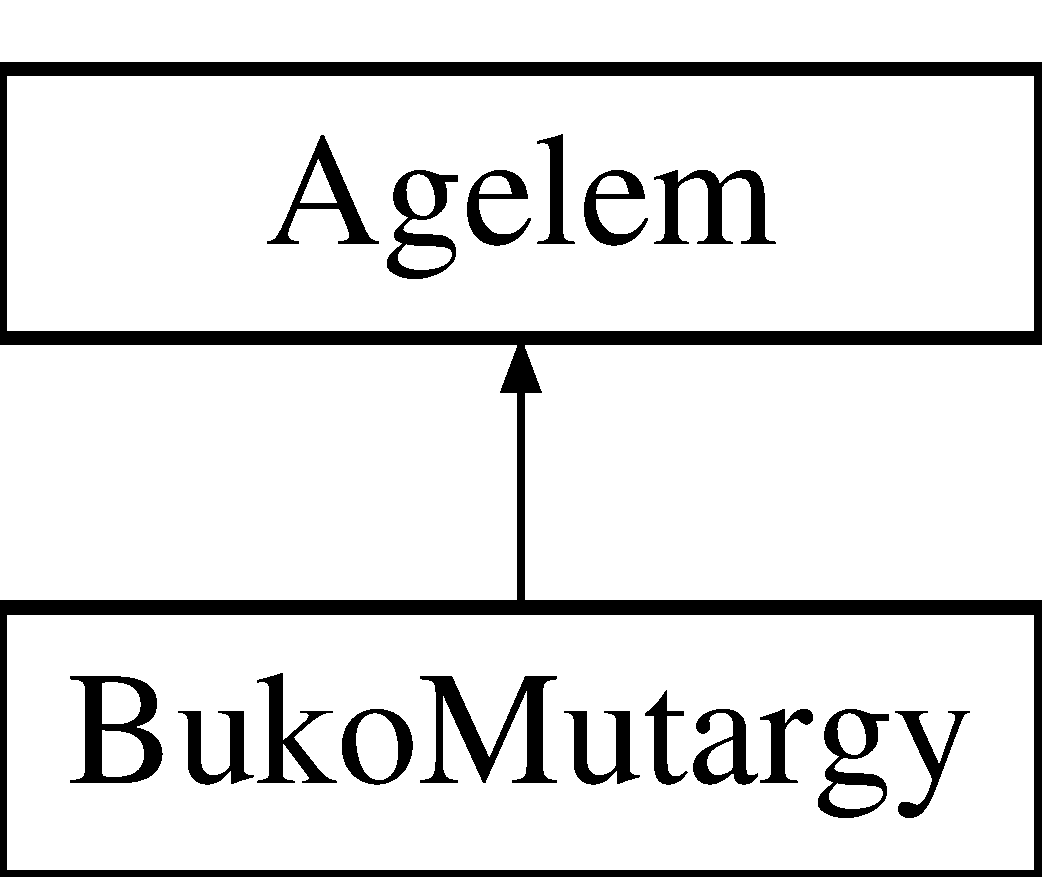
\includegraphics[height=2.000000cm]{class_buko_mutargy}
\end{center}
\end{figure}
\subsection*{Public Member Functions}
\begin{DoxyCompactItemize}
\item 
\mbox{\Hypertarget{class_buko_mutargy_ae4ce2dece863cab87563635402c393c1}\label{class_buko_mutargy_ae4ce2dece863cab87563635402c393c1}} 
\hyperlink{class_buko_mutargy_ae4ce2dece863cab87563635402c393c1}{Buko\+Mutargy} (const string \hyperlink{class_agelem_abe92b7e3912367d5d1caf6b277ca0b7d}{nev}, const string a\+\_\+cspe\+\_\+nev, const string a\+\_\+cspv\+\_\+nev, const double a\+\_\+ro, const double \hyperlink{class_agelem_a3f8668febc2958fd539997d537552f17}{Aref}, const double Hf, const bool is\+\_\+opened, const double width, const double overflow\+\_\+height, const double discharge\+\_\+coeff, const double valve\+\_\+coeff, const double a\+\_\+mp)
\begin{DoxyCompactList}\small\item\em Konstruktor. \end{DoxyCompactList}\item 
\mbox{\Hypertarget{class_buko_mutargy_a27d37980ab52769b2d0f0864e7eb4a62}\label{class_buko_mutargy_a27d37980ab52769b2d0f0864e7eb4a62}} 
\hyperlink{class_buko_mutargy_a27d37980ab52769b2d0f0864e7eb4a62}{$\sim$\+Buko\+Mutargy} ()
\begin{DoxyCompactList}\small\item\em Destruktor. \end{DoxyCompactList}\item 
\mbox{\Hypertarget{class_buko_mutargy_ab25d69cf3cf673e44252b9f22c99bc86}\label{class_buko_mutargy_ab25d69cf3cf673e44252b9f22c99bc86}} 
string \hyperlink{class_buko_mutargy_ab25d69cf3cf673e44252b9f22c99bc86}{Info} ()
\begin{DoxyCompactList}\small\item\em Inform�ci� \end{DoxyCompactList}\item 
\mbox{\Hypertarget{class_buko_mutargy_a917e0bf2e4aec1e29fc243b27d80400f}\label{class_buko_mutargy_a917e0bf2e4aec1e29fc243b27d80400f}} 
double \hyperlink{class_buko_mutargy_a917e0bf2e4aec1e29fc243b27d80400f}{f} (vector$<$ double $>$)
\begin{DoxyCompactList}\small\item\em �gegyenlet �rt�ke. \end{DoxyCompactList}\item 
\mbox{\Hypertarget{class_buko_mutargy_a512f96bd4ea56e9cd5a29662382b23ae}\label{class_buko_mutargy_a512f96bd4ea56e9cd5a29662382b23ae}} 
vector$<$ double $>$ \hyperlink{class_buko_mutargy_a512f96bd4ea56e9cd5a29662382b23ae}{df} (vector$<$ double $>$)
\begin{DoxyCompactList}\small\item\em �gegyenlet linariz�ltja. \end{DoxyCompactList}\item 
\mbox{\Hypertarget{class_buko_mutargy_ab54be1629d47cbcec4bc5a389323a234}\label{class_buko_mutargy_ab54be1629d47cbcec4bc5a389323a234}} 
void \hyperlink{class_buko_mutargy_ab54be1629d47cbcec4bc5a389323a234}{Ini} (int mode, double value)
\begin{DoxyCompactList}\small\item\em Inicializ�ci� \end{DoxyCompactList}\item 
\mbox{\Hypertarget{class_buko_mutargy_a2b9a66ad0547199dab8a31c04a0c714f}\label{class_buko_mutargy_a2b9a66ad0547199dab8a31c04a0c714f}} 
string \hyperlink{class_buko_mutargy_a2b9a66ad0547199dab8a31c04a0c714f}{Get\+Type} ()
\begin{DoxyCompactList}\small\item\em Keresztmetszeti jellemzok szamitasa. \end{DoxyCompactList}\item 
\mbox{\Hypertarget{class_buko_mutargy_af8e1ff9aa34978d92be2c258f7b0a056}\label{class_buko_mutargy_af8e1ff9aa34978d92be2c258f7b0a056}} 
void {\bfseries Set\+\_\+dprop} (string mit, double mire)
\item 
\mbox{\Hypertarget{class_buko_mutargy_a0e6c4884543cdd94e0905e0e64561f5f}\label{class_buko_mutargy_a0e6c4884543cdd94e0905e0e64561f5f}} 
double \hyperlink{class_buko_mutargy_a0e6c4884543cdd94e0905e0e64561f5f}{Get\+\_\+dprop} (string mit)
\begin{DoxyCompactList}\small\item\em Get double property, \hyperlink{class_cso}{Cso} es \hyperlink{class_csatorna}{Csatorna} akarja elulirja. \end{DoxyCompactList}\end{DoxyCompactItemize}
\subsection*{Additional Inherited Members}


The documentation for this class was generated from the following files\+:\begin{DoxyCompactItemize}
\item 
Buko\+Mutargy.\+h\item 
Buko\+Mutargy.\+cpp\end{DoxyCompactItemize}

\hypertarget{class_csatorna}{}\section{Csatorna Class Reference}
\label{class_csatorna}\index{Csatorna@{Csatorna}}
Inheritance diagram for Csatorna\+:\begin{figure}[H]
\begin{center}
\leavevmode
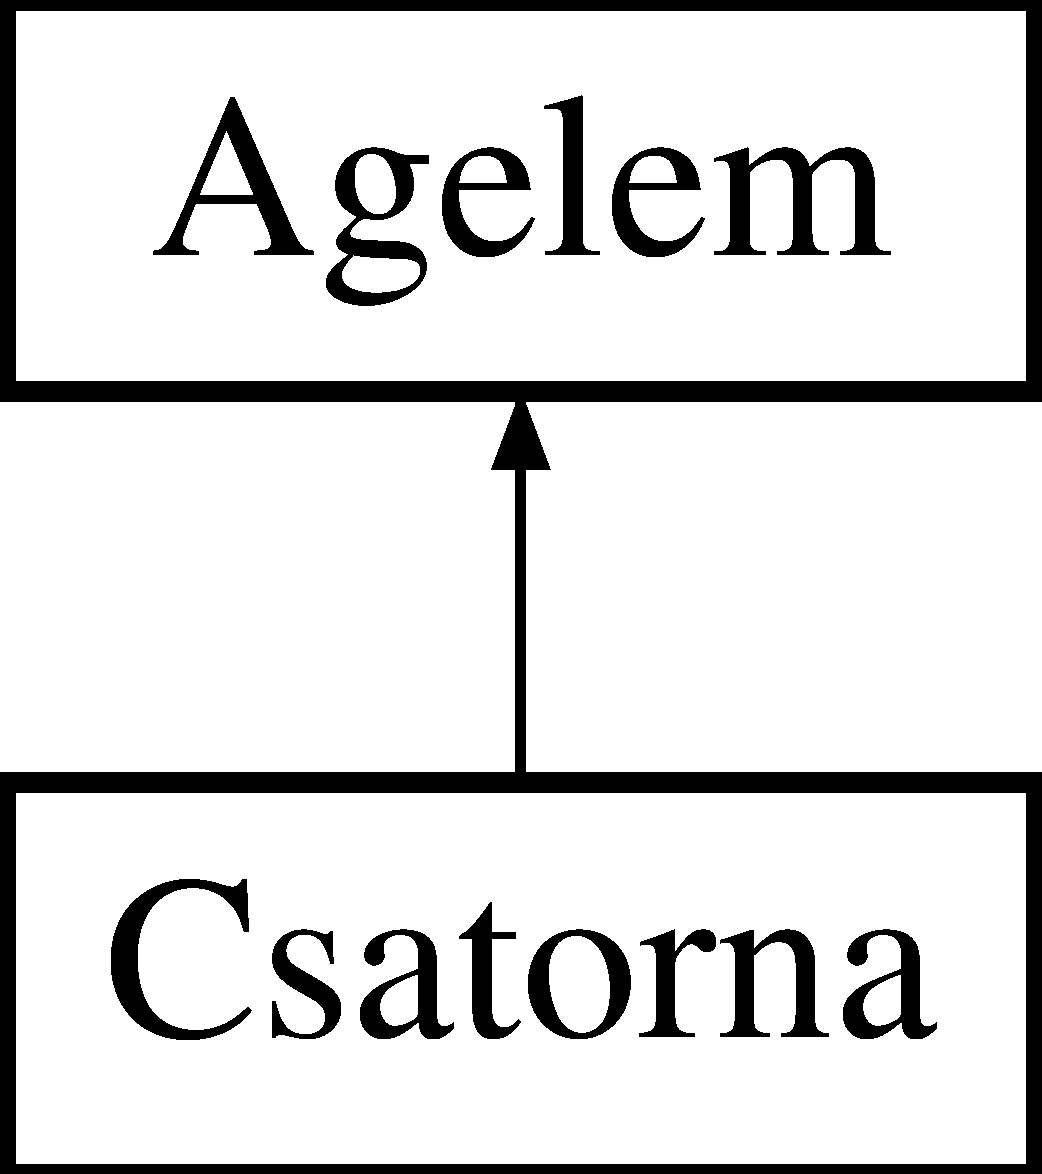
\includegraphics[height=2.000000cm]{class_csatorna}
\end{center}
\end{figure}
\subsection*{Public Member Functions}
\begin{DoxyCompactItemize}
\item 
\hyperlink{class_csatorna_ae3829a74761e0507363290fde29af12b}{Csatorna} (const string \hyperlink{class_agelem_abe92b7e3912367d5d1caf6b277ca0b7d}{nev}, const string a\+\_\+cspe\+\_\+nev, const string a\+\_\+cspv\+\_\+nev, const double a\+\_\+ro, const double \hyperlink{class_agelem_a3f8668febc2958fd539997d537552f17}{Aref}, const double L, const double ze, const double zv, const double surl, const int int\+\_\+steps, const int debugl, const double dia, const double a\+\_\+cl\+\_\+k, const double a\+\_\+cl\+\_\+w, const bool is\+\_\+reversed, const double a\+\_\+mp)
\begin{DoxyCompactList}\small\item\em Konstruktor t�glalap km. eset�n. \end{DoxyCompactList}\item 
\hyperlink{class_csatorna_a84452f3df42df853e0600d383cd37d8a}{$\sim$\+Csatorna} ()
\begin{DoxyCompactList}\small\item\em Konstruktor user-\/defined km. eset�n. \end{DoxyCompactList}\item 
string \hyperlink{class_csatorna_a77f24ff76c738a89cb827d251fec0845}{Info} ()
\begin{DoxyCompactList}\small\item\em Inform�ci� \end{DoxyCompactList}\item 
double \hyperlink{class_csatorna_a5cd4e0975717ce0baab89f57a566782a}{f} (vector$<$ double $>$)
\begin{DoxyCompactList}\small\item\em �gegyenlet �rt�ke \end{DoxyCompactList}\item 
vector$<$ double $>$ \hyperlink{class_csatorna_a5330dbbbc669f49382c822ffcc671d16}{df} (vector$<$ double $>$)
\begin{DoxyCompactList}\small\item\em �gegyenlet derv�ltja \end{DoxyCompactList}\item 
void \hyperlink{class_csatorna_ab30adea649ae8708061e211dc450cb06}{Ini} (int mode, double value)
\begin{DoxyCompactList}\small\item\em Inicializ�ci� \end{DoxyCompactList}\item 
void \hyperlink{class_csatorna_ab9528187fc3d40d210c85b72d7856f10}{keresztmetszet} (const double y, double \&A, double \&B, double \&Rh)
\begin{DoxyCompactList}\small\item\em Keresztmetszeti jellemzok szamitasa. \end{DoxyCompactList}\item 
\mbox{\Hypertarget{class_csatorna_af30a5d124d26bd31548cf243c4a95178}\label{class_csatorna_af30a5d124d26bd31548cf243c4a95178}} 
void \hyperlink{class_csatorna_af30a5d124d26bd31548cf243c4a95178}{norm\+\_\+krit} (const double Q)
\begin{DoxyCompactList}\small\item\em Norm�l-\/ �s kritikus szint sz�m�t�sa adott t�rfogat�ramhoz. \end{DoxyCompactList}\item 
double \hyperlink{class_csatorna_aacea0461de03c4592e89cee026c2e1d5}{nyf\+\_\+ode} (const double x, const double y, const double \hyperlink{class_agelem_a1377d80d8511cc4adacccba31d28282d}{mp})
\begin{DoxyCompactList}\small\item\em A ny�ltfelsz�n� �raml�s le�r� DE. \end{DoxyCompactList}\item 
double \hyperlink{class_csatorna_a17e55cbde88d58985f7e315e7069ba3a}{ode\+\_\+megoldo} (double ystart, double dx, double xstart, double \hyperlink{class_agelem_a1377d80d8511cc4adacccba31d28282d}{mp})
\begin{DoxyCompactList}\small\item\em O\+DE integr�l�s. \end{DoxyCompactList}\item 
void \hyperlink{class_csatorna_a2ad82029529f1aa2b4da3122b608eb6c}{compute\+\_\+distr} ()
\begin{DoxyCompactList}\small\item\em Az eredmenyeloszlasok elkeszitese. \end{DoxyCompactList}\item 
\mbox{\Hypertarget{class_csatorna_ab515ee9bcf30c35c22b23fd0617cc422}\label{class_csatorna_ab515ee9bcf30c35c22b23fd0617cc422}} 
vector$<$ double $>$ \hyperlink{class_csatorna_ab515ee9bcf30c35c22b23fd0617cc422}{Get\+\_\+res} (string mit)
\begin{DoxyCompactList}\small\item\em Eredm�nyeloszl�sok visszaad�sa. \end{DoxyCompactList}\item 
\mbox{\Hypertarget{class_csatorna_a8ca44a377b12883ddad100f0dea9aed2}\label{class_csatorna_a8ca44a377b12883ddad100f0dea9aed2}} 
double \hyperlink{class_csatorna_a8ca44a377b12883ddad100f0dea9aed2}{surlodas} ()
\begin{DoxyCompactList}\small\item\em Surl�dosi modell. \end{DoxyCompactList}\item 
\mbox{\Hypertarget{class_csatorna_a581b69e57becd825b645f07b07028051}\label{class_csatorna_a581b69e57becd825b645f07b07028051}} 
double \hyperlink{class_csatorna_a581b69e57becd825b645f07b07028051}{Get\+\_\+dprop} (string mit)
\begin{DoxyCompactList}\small\item\em Get Double property. \end{DoxyCompactList}\item 
\mbox{\Hypertarget{class_csatorna_a256060fc76bcee088250b0810eaadabb}\label{class_csatorna_a256060fc76bcee088250b0810eaadabb}} 
double \hyperlink{class_csatorna_a256060fc76bcee088250b0810eaadabb}{Get\+\_\+\+Foly\+Terf} ()
\begin{DoxyCompactList}\small\item\em Folyadekterfogat az elemben. \end{DoxyCompactList}\item 
void \hyperlink{class_csatorna_a765dd9b66d2a18b567a6045d17266a10}{error} (string fv, string msg)
\begin{DoxyCompactList}\small\item\em Hibauzenet. \end{DoxyCompactList}\item 
void \hyperlink{class_csatorna_ac2000669171af7d8fa5f447cb8aa231d}{warning} (string fv, string msg)
\begin{DoxyCompactList}\small\item\em Figyelmeztetes. \end{DoxyCompactList}\item 
\mbox{\Hypertarget{class_csatorna_a6b1b895f6b560b8bb3a517c48b12210e}\label{class_csatorna_a6b1b895f6b560b8bb3a517c48b12210e}} 
string {\bfseries Get\+Type} ()
\item 
\mbox{\Hypertarget{class_csatorna_aa1895b07dd2d4b836f0efbe0869cd4e1}\label{class_csatorna_aa1895b07dd2d4b836f0efbe0869cd4e1}} 
void {\bfseries Set\+\_\+dprop} (string mit, double mire)
\item 
\mbox{\Hypertarget{class_csatorna_a74db8402dcaaf02c408c1ac900a610f9}\label{class_csatorna_a74db8402dcaaf02c408c1ac900a610f9}} 
virtual double \hyperlink{class_csatorna_a74db8402dcaaf02c408c1ac900a610f9}{Get\+\_\+v} ()
\begin{DoxyCompactList}\small\item\em Overriding Agelem\+::\+Set\+Log\+File() \end{DoxyCompactList}\item 
\mbox{\Hypertarget{class_csatorna_afc26b196d6234c18ed3e1529390a10b5}\label{class_csatorna_afc26b196d6234c18ed3e1529390a10b5}} 
bool {\bfseries Get\+\_\+res\+\_\+ready} ()
\end{DoxyCompactItemize}
\subsection*{Additional Inherited Members}


\subsection{Constructor \& Destructor Documentation}
\mbox{\Hypertarget{class_csatorna_ae3829a74761e0507363290fde29af12b}\label{class_csatorna_ae3829a74761e0507363290fde29af12b}} 
\index{Csatorna@{Csatorna}!Csatorna@{Csatorna}}
\index{Csatorna@{Csatorna}!Csatorna@{Csatorna}}
\subsubsection{\texorpdfstring{Csatorna()}{Csatorna()}}
{\footnotesize\ttfamily Csatorna\+::\+Csatorna (\begin{DoxyParamCaption}\item[{const string}]{nev,  }\item[{const string}]{a\+\_\+cspe\+\_\+nev,  }\item[{const string}]{a\+\_\+cspv\+\_\+nev,  }\item[{const double}]{a\+\_\+ro,  }\item[{const double}]{Aref,  }\item[{const double}]{L,  }\item[{const double}]{ze,  }\item[{const double}]{zv,  }\item[{const double}]{surl,  }\item[{const int}]{int\+\_\+steps,  }\item[{const int}]{debugl,  }\item[{const double}]{dia,  }\item[{const double}]{a\+\_\+cl\+\_\+k,  }\item[{const double}]{a\+\_\+cl\+\_\+w,  }\item[{const bool}]{is\+\_\+reversed,  }\item[{const double}]{a\+\_\+mp }\end{DoxyParamCaption})}



Konstruktor t�glalap km. eset�n. 

K�r km.

Konstruktor k�r km. eset�n \mbox{\Hypertarget{class_csatorna_a84452f3df42df853e0600d383cd37d8a}\label{class_csatorna_a84452f3df42df853e0600d383cd37d8a}} 
\index{Csatorna@{Csatorna}!````~Csatorna@{$\sim$\+Csatorna}}
\index{````~Csatorna@{$\sim$\+Csatorna}!Csatorna@{Csatorna}}
\subsubsection{\texorpdfstring{$\sim$\+Csatorna()}{~Csatorna()}}
{\footnotesize\ttfamily Csatorna\+::$\sim$\+Csatorna (\begin{DoxyParamCaption}{ }\end{DoxyParamCaption})}



Konstruktor user-\/defined km. eset�n. 

Destruktor 

\subsection{Member Function Documentation}
\mbox{\Hypertarget{class_csatorna_a2ad82029529f1aa2b4da3122b608eb6c}\label{class_csatorna_a2ad82029529f1aa2b4da3122b608eb6c}} 
\index{Csatorna@{Csatorna}!compute\+\_\+distr@{compute\+\_\+distr}}
\index{compute\+\_\+distr@{compute\+\_\+distr}!Csatorna@{Csatorna}}
\subsubsection{\texorpdfstring{compute\+\_\+distr()}{compute\_distr()}}
{\footnotesize\ttfamily void Csatorna\+::compute\+\_\+distr (\begin{DoxyParamCaption}{ }\end{DoxyParamCaption})}



Az eredmenyeloszlasok elkeszitese. 

debug f�jl �r�sa void logfile\+\_\+write(string msg, int msg\+\_\+debug\+\_\+level); \mbox{\Hypertarget{class_csatorna_a5330dbbbc669f49382c822ffcc671d16}\label{class_csatorna_a5330dbbbc669f49382c822ffcc671d16}} 
\index{Csatorna@{Csatorna}!df@{df}}
\index{df@{df}!Csatorna@{Csatorna}}
\subsubsection{\texorpdfstring{df()}{df()}}
{\footnotesize\ttfamily vector$<$ double $>$ Csatorna\+::df (\begin{DoxyParamCaption}\item[{vector$<$ double $>$}]{x }\end{DoxyParamCaption})\hspace{0.3cm}{\ttfamily [virtual]}}



�gegyenlet derv�ltja 

�gegyenlet deriv�ltjai (sz�m�t�s\+:

\begin{DoxySeeAlso}{See also}
\hyperlink{class_csatorna_a5cd4e0975717ce0baab89f57a566782a}{f}) 
\end{DoxySeeAlso}
\begin{DoxyReturn}{Returns}
df �rt�ke 
\end{DoxyReturn}


Implements \hyperlink{class_agelem_a7934ea6320bdc37526ed3daa108ce1ed}{Agelem}.

\mbox{\Hypertarget{class_csatorna_a765dd9b66d2a18b567a6045d17266a10}\label{class_csatorna_a765dd9b66d2a18b567a6045d17266a10}} 
\index{Csatorna@{Csatorna}!error@{error}}
\index{error@{error}!Csatorna@{Csatorna}}
\subsubsection{\texorpdfstring{error()}{error()}}
{\footnotesize\ttfamily void Csatorna\+::error (\begin{DoxyParamCaption}\item[{string}]{fv,  }\item[{string}]{msg }\end{DoxyParamCaption})}



Hibauzenet. 

Hibauzenet k�perny�re �s eredm�nyf�jlba.


\begin{DoxyParams}{Parameters}
{\em fv} & h�v� f�ggv�ny \\
\hline
{\em msg} & �zenet \\
\hline
\end{DoxyParams}
\mbox{\Hypertarget{class_csatorna_a5cd4e0975717ce0baab89f57a566782a}\label{class_csatorna_a5cd4e0975717ce0baab89f57a566782a}} 
\index{Csatorna@{Csatorna}!f@{f}}
\index{f@{f}!Csatorna@{Csatorna}}
\subsubsection{\texorpdfstring{f()}{f()}}
{\footnotesize\ttfamily double Csatorna\+::f (\begin{DoxyParamCaption}\item[{vector$<$ double $>$}]{x }\end{DoxyParamCaption})\hspace{0.3cm}{\ttfamily [virtual]}}



�gegyenlet �rt�ke 

�gegyenlet �s deriv�ltak sz�m�t�sa


\begin{DoxyParams}{Parameters}
{\em x\mbox{[}0\mbox{]}} & = pe/ro/g -\/ nyom�s \mbox{[}v.\+o.\+m.\mbox{]} az �gelem elej�n \\
\hline
{\em x\mbox{[}1\mbox{]}} & = pv/ro/g -\/ nyom�s \mbox{[}v.\+o.\+m.\mbox{]} az �gelem v�g�n \\
\hline
{\em x\mbox{[}2\mbox{]}} & = he/ro/g -\/ �gelem elej�n a csom�pont nullszintje \mbox{[}m\mbox{]} \\
\hline
{\em x\mbox{[}3\mbox{]}} & = hv/ro/g -\/ �gelem v�g�n a csom�pont nullszintje \mbox{[}m\mbox{]} \\
\hline
\end{DoxyParams}
\begin{DoxyReturn}{Returns}
f �rt�ke
\end{DoxyReturn}
�gelem elej�n az abszol�t nyom�sszint\+: he(aknafen�k) + pe/ro/g = x\mbox{[}0\mbox{]}+x\mbox{[}1\mbox{]} �gelem elej�n az abszol�t nyom�sszint\+: hv(aknafen�k) + pv/ro/g = x\mbox{[}0\mbox{]}+x\mbox{[}1\mbox{]}

Az elj�r�s kisz�m�tja a deriv�ltakat is, �gy \begin{DoxySeeAlso}{See also}
\hyperlink{class_csatorna_a5330dbbbc669f49382c822ffcc671d16}{df} csak visszaadja az �rt�ket. 
\end{DoxySeeAlso}


Implements \hyperlink{class_agelem_aa1d93be52ddae11df003c4e35c47084b}{Agelem}.

\mbox{\Hypertarget{class_csatorna_a77f24ff76c738a89cb827d251fec0845}\label{class_csatorna_a77f24ff76c738a89cb827d251fec0845}} 
\index{Csatorna@{Csatorna}!Info@{Info}}
\index{Info@{Info}!Csatorna@{Csatorna}}
\subsubsection{\texorpdfstring{Info()}{Info()}}
{\footnotesize\ttfamily string Csatorna\+::\+Info (\begin{DoxyParamCaption}{ }\end{DoxyParamCaption})\hspace{0.3cm}{\ttfamily [virtual]}}



Inform�ci� 

Info.

\begin{DoxyReturn}{Returns}
info string 
\end{DoxyReturn}


Reimplemented from \hyperlink{class_agelem_a2e6c4688cdbdf17c6d3bde0c6c08ff49}{Agelem}.

\mbox{\Hypertarget{class_csatorna_ab30adea649ae8708061e211dc450cb06}\label{class_csatorna_ab30adea649ae8708061e211dc450cb06}} 
\index{Csatorna@{Csatorna}!Ini@{Ini}}
\index{Ini@{Ini}!Csatorna@{Csatorna}}
\subsubsection{\texorpdfstring{Ini()}{Ini()}}
{\footnotesize\ttfamily void Csatorna\+::\+Ini (\begin{DoxyParamCaption}\item[{int}]{mode,  }\item[{double}]{value }\end{DoxyParamCaption})\hspace{0.3cm}{\ttfamily [virtual]}}



Inicializ�ci� 

�gelem inicializ�l�sa


\begin{DoxyParams}{Parameters}
{\em mode} & -\/ (0) automatikus, (1) mp=value \\
\hline
{\em value} & csak mode=1 eset�n \\
\hline
\end{DoxyParams}


Implements \hyperlink{class_agelem_a844171faf01143770bbd894b1a48e72f}{Agelem}.

\mbox{\Hypertarget{class_csatorna_ab9528187fc3d40d210c85b72d7856f10}\label{class_csatorna_ab9528187fc3d40d210c85b72d7856f10}} 
\index{Csatorna@{Csatorna}!keresztmetszet@{keresztmetszet}}
\index{keresztmetszet@{keresztmetszet}!Csatorna@{Csatorna}}
\subsubsection{\texorpdfstring{keresztmetszet()}{keresztmetszet()}}
{\footnotesize\ttfamily void Csatorna\+::keresztmetszet (\begin{DoxyParamCaption}\item[{const double}]{yy,  }\item[{double \&}]{A,  }\item[{double \&}]{B,  }\item[{double \&}]{Rh }\end{DoxyParamCaption})}



Keresztmetszeti jellemzok szamitasa. 

Keresztmetszeti jellemz�k sz�m�t�sa.


\begin{DoxyParams}{Parameters}
{\em y} & v�zszint \\
\hline
{\em \&A} & nedves�tett ter�let \\
\hline
{\em \&B} & nedves�tett ker�let \\
\hline
{\em \&\+Rh} & hidraulikai sug�r (A/B) \\
\hline
\end{DoxyParams}
\mbox{\Hypertarget{class_csatorna_aacea0461de03c4592e89cee026c2e1d5}\label{class_csatorna_aacea0461de03c4592e89cee026c2e1d5}} 
\index{Csatorna@{Csatorna}!nyf\+\_\+ode@{nyf\+\_\+ode}}
\index{nyf\+\_\+ode@{nyf\+\_\+ode}!Csatorna@{Csatorna}}
\subsubsection{\texorpdfstring{nyf\+\_\+ode()}{nyf\_ode()}}
{\footnotesize\ttfamily double Csatorna\+::nyf\+\_\+ode (\begin{DoxyParamCaption}\item[{const double}]{x,  }\item[{const double}]{y,  }\item[{const double}]{mp }\end{DoxyParamCaption})}



A ny�ltfelsz�n� �raml�s le�r� DE. 

Folyad�kfelsz�nt le�r� dy/dx=f(x,y) K\+DE jobboldala.


\begin{DoxyParams}{Parameters}
{\em x} & x koordin�ta \\
\hline
{\em y} & y koordin�ta \\
\hline
\end{DoxyParams}
\begin{DoxyReturn}{Returns}
dy/dx �rt�ke 
\end{DoxyReturn}
\mbox{\Hypertarget{class_csatorna_a17e55cbde88d58985f7e315e7069ba3a}\label{class_csatorna_a17e55cbde88d58985f7e315e7069ba3a}} 
\index{Csatorna@{Csatorna}!ode\+\_\+megoldo@{ode\+\_\+megoldo}}
\index{ode\+\_\+megoldo@{ode\+\_\+megoldo}!Csatorna@{Csatorna}}
\subsubsection{\texorpdfstring{ode\+\_\+megoldo()}{ode\_megoldo()}}
{\footnotesize\ttfamily double Csatorna\+::ode\+\_\+megoldo (\begin{DoxyParamCaption}\item[{double}]{y0,  }\item[{double}]{dx0,  }\item[{double}]{x0,  }\item[{double}]{mp }\end{DoxyParamCaption})}



O\+DE integr�l�s. 

O\+DE solver.


\begin{DoxyParams}{Parameters}
{\em y0} & depth at x=0 \\
\hline
{\em dx0} & initial dx step \\
\hline
{\em x0} & initial x value (defines direction of integration) \\
\hline
\end{DoxyParams}
\begin{DoxyReturn}{Returns}
y result of integration 
\end{DoxyReturn}
\mbox{\Hypertarget{class_csatorna_ac2000669171af7d8fa5f447cb8aa231d}\label{class_csatorna_ac2000669171af7d8fa5f447cb8aa231d}} 
\index{Csatorna@{Csatorna}!warning@{warning}}
\index{warning@{warning}!Csatorna@{Csatorna}}
\subsubsection{\texorpdfstring{warning()}{warning()}}
{\footnotesize\ttfamily void Csatorna\+::warning (\begin{DoxyParamCaption}\item[{string}]{fv,  }\item[{string}]{msg }\end{DoxyParamCaption})}



Figyelmeztetes. 

Figyelmeztetes k�perny�re �s eredm�nyf�jlba.


\begin{DoxyParams}{Parameters}
{\em fv} & h�v� f�ggv�ny \\
\hline
{\em msg} & �zenet \\
\hline
\end{DoxyParams}


The documentation for this class was generated from the following files\+:\begin{DoxyCompactItemize}
\item 
Csatorna.\+h\item 
Csatorna.\+cpp\end{DoxyCompactItemize}

\hypertarget{class_cso}{}\section{Cso Class Reference}
\label{class_cso}\index{Cso@{Cso}}
Inheritance diagram for Cso\+:\begin{figure}[H]
\begin{center}
\leavevmode
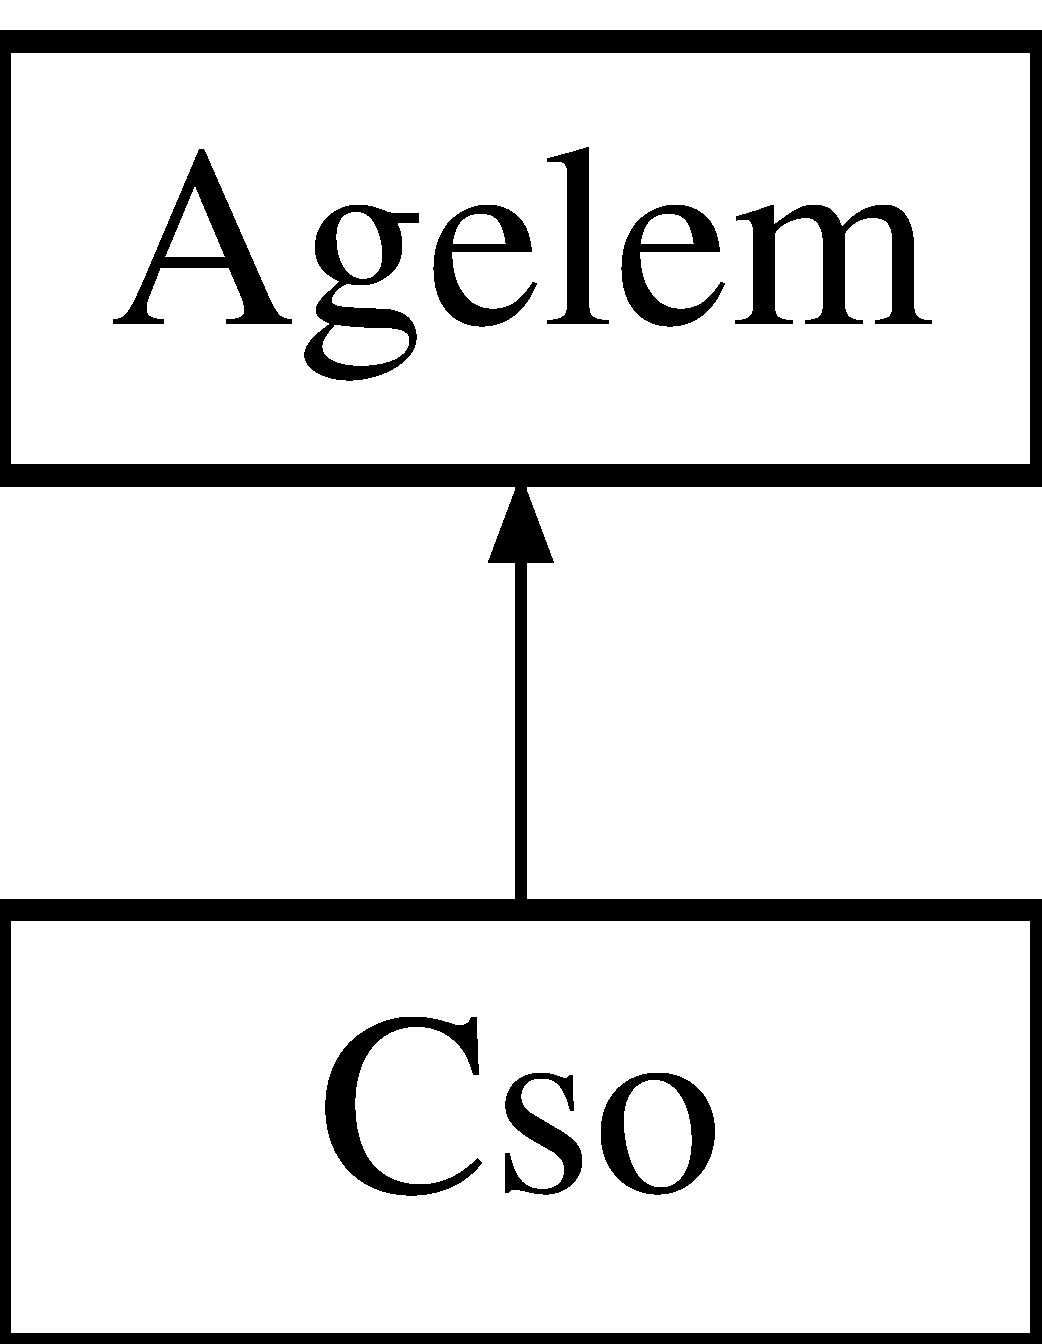
\includegraphics[height=2.000000cm]{class_cso}
\end{center}
\end{figure}
\subsection*{Public Member Functions}
\begin{DoxyCompactItemize}
\item 
\mbox{\Hypertarget{class_cso_ab04f2170382860dcff777b7185c62ba7}\label{class_cso_ab04f2170382860dcff777b7185c62ba7}} 
{\bfseries Cso} (const string \hyperlink{class_agelem_abe92b7e3912367d5d1caf6b277ca0b7d}{nev}, const string a\+\_\+cspe\+\_\+nev, const string a\+\_\+cspv\+\_\+nev, const double a\+\_\+ro, const double L, const double D, const double lambda, const double cl\+\_\+k, const double cl\+\_\+w, const double \hyperlink{class_agelem_a1377d80d8511cc4adacccba31d28282d}{mp})
\item 
\mbox{\Hypertarget{class_cso_af6a08482d5949b0924459b7588efd2a0}\label{class_cso_af6a08482d5949b0924459b7588efd2a0}} 
string \hyperlink{class_cso_af6a08482d5949b0924459b7588efd2a0}{Info} ()
\begin{DoxyCompactList}\small\item\em Informacio. \end{DoxyCompactList}\item 
\mbox{\Hypertarget{class_cso_a5b0e37d3a2f6095e958a7c5f27d8e060}\label{class_cso_a5b0e37d3a2f6095e958a7c5f27d8e060}} 
double \hyperlink{class_cso_a5b0e37d3a2f6095e958a7c5f27d8e060}{f} (vector$<$ double $>$)
\begin{DoxyCompactList}\small\item\em Az agegyenlet erteke, nullara rendezve, v.\+o.\+m.-\/ben. \end{DoxyCompactList}\item 
\mbox{\Hypertarget{class_cso_acc0b1bb6f9558475a097219d88d07267}\label{class_cso_acc0b1bb6f9558475a097219d88d07267}} 
vector$<$ double $>$ \hyperlink{class_cso_acc0b1bb6f9558475a097219d88d07267}{df} (vector$<$ double $>$)
\begin{DoxyCompactList}\small\item\em Jacobi\+: df/dhe, df/dhv, df/dmp, konstans tag. \end{DoxyCompactList}\item 
\mbox{\Hypertarget{class_cso_aad51dd17829b413a41f1afb0c275d55c}\label{class_cso_aad51dd17829b413a41f1afb0c275d55c}} 
void \hyperlink{class_cso_aad51dd17829b413a41f1afb0c275d55c}{Ini} (int mode, double value)
\begin{DoxyCompactList}\small\item\em Inicializacio, mode=0 -\/$>$ automatikus, mode=1 -\/$>$ value beirasa. \end{DoxyCompactList}\item 
double \hyperlink{class_cso_a01d6ba01b924fe317638fe196a139d1f}{surlodas} ()
\begin{DoxyCompactList}\small\item\em Sets the friction coefficient lambda. \end{DoxyCompactList}\item 
\mbox{\Hypertarget{class_cso_a674c356a597eb9d6c9a46726b35e2a00}\label{class_cso_a674c356a597eb9d6c9a46726b35e2a00}} 
double \hyperlink{class_cso_a674c356a597eb9d6c9a46726b35e2a00}{Get\+\_\+dprop} (string mit)
\begin{DoxyCompactList}\small\item\em Get double property, \hyperlink{class_cso}{Cso} es \hyperlink{class_csatorna}{Csatorna} akarja elulirja. \end{DoxyCompactList}\item 
\mbox{\Hypertarget{class_cso_a794959559cb679efb0529417e1df6556}\label{class_cso_a794959559cb679efb0529417e1df6556}} 
double \hyperlink{class_cso_a794959559cb679efb0529417e1df6556}{Get\+\_\+dfdmu} (string mit)
\begin{DoxyCompactList}\small\item\em Get equation derivative w.\+r.\+t. parameter. \end{DoxyCompactList}\item 
\mbox{\Hypertarget{class_cso_ae6db4734838a6261e89caeb53269e990}\label{class_cso_ae6db4734838a6261e89caeb53269e990}} 
void {\bfseries Set\+\_\+dprop} (string mit, double mire)
\item 
\mbox{\Hypertarget{class_cso_a20b7469a9b992da3bc25c647cdfa23c8}\label{class_cso_a20b7469a9b992da3bc25c647cdfa23c8}} 
string {\bfseries Get\+Type} ()
\item 
double \hyperlink{class_cso_a796d4ff0f69732001c91abe7e5ce7ed7}{Compute\+Headloss} ()
\begin{DoxyCompactList}\small\item\em Computes the head loss in Pa. \end{DoxyCompactList}\item 
double \hyperlink{class_cso_a5f8536643bc971ca70aebef850fa53a1}{Compute\+Headloss\+Derivative} ()
\begin{DoxyCompactList}\small\item\em Computes the head loss derivative w.\+r.\+t. mass flow rate. \end{DoxyCompactList}\item 
void \hyperlink{class_cso_a113196b16e49417924fea36b770f4d84}{Set\+\_\+friction\+\_\+model} (string friction\+\_\+model)
\begin{DoxyCompactList}\small\item\em Sets the friction model. \end{DoxyCompactList}\end{DoxyCompactItemize}
\subsection*{Additional Inherited Members}


\subsection{Member Function Documentation}
\mbox{\Hypertarget{class_cso_a796d4ff0f69732001c91abe7e5ce7ed7}\label{class_cso_a796d4ff0f69732001c91abe7e5ce7ed7}} 
\index{Cso@{Cso}!Compute\+Headloss@{Compute\+Headloss}}
\index{Compute\+Headloss@{Compute\+Headloss}!Cso@{Cso}}
\subsubsection{\texorpdfstring{Compute\+Headloss()}{ComputeHeadloss()}}
{\footnotesize\ttfamily double Cso\+::\+Compute\+Headloss (\begin{DoxyParamCaption}{ }\end{DoxyParamCaption})}



Computes the head loss in Pa. 

dp\textquotesingle{}=lambda$\ast$\+L/\+D$\ast$ro/2$\ast$v$\ast$fabs(v) \mbox{\Hypertarget{class_cso_a5f8536643bc971ca70aebef850fa53a1}\label{class_cso_a5f8536643bc971ca70aebef850fa53a1}} 
\index{Cso@{Cso}!Compute\+Headloss\+Derivative@{Compute\+Headloss\+Derivative}}
\index{Compute\+Headloss\+Derivative@{Compute\+Headloss\+Derivative}!Cso@{Cso}}
\subsubsection{\texorpdfstring{Compute\+Headloss\+Derivative()}{ComputeHeadlossDerivative()}}
{\footnotesize\ttfamily double Cso\+::\+Compute\+Headloss\+Derivative (\begin{DoxyParamCaption}{ }\end{DoxyParamCaption})}



Computes the head loss derivative w.\+r.\+t. mass flow rate. 

dp\textquotesingle{}=lambda$\ast$\+L/\+D$\ast$ro/2$\ast$v$\ast$fabs(v) d dp\textquotesingle{}/dmp=lambda$\ast$\+L/\+D$\ast$ro/2$\ast$1/(ro$\ast$A)$^\wedge$2$\ast$abs(v) \mbox{\Hypertarget{class_cso_a113196b16e49417924fea36b770f4d84}\label{class_cso_a113196b16e49417924fea36b770f4d84}} 
\index{Cso@{Cso}!Set\+\_\+friction\+\_\+model@{Set\+\_\+friction\+\_\+model}}
\index{Set\+\_\+friction\+\_\+model@{Set\+\_\+friction\+\_\+model}!Cso@{Cso}}
\subsubsection{\texorpdfstring{Set\+\_\+friction\+\_\+model()}{Set\_friction\_model()}}
{\footnotesize\ttfamily void Cso\+::\+Set\+\_\+friction\+\_\+model (\begin{DoxyParamCaption}\item[{string}]{a\+\_\+fric\+\_\+type }\end{DoxyParamCaption})\hspace{0.3cm}{\ttfamily [virtual]}}



Sets the friction model. 

DW (friction\+\_\+model\+\_\+type = 0) -\/$>$ Darcy Wiesenbach HW (friction\+\_\+model\+\_\+type = 1) -\/$>$ Hazen-\/\+Williams 

Reimplemented from \hyperlink{class_agelem}{Agelem}.

\mbox{\Hypertarget{class_cso_a01d6ba01b924fe317638fe196a139d1f}\label{class_cso_a01d6ba01b924fe317638fe196a139d1f}} 
\index{Cso@{Cso}!surlodas@{surlodas}}
\index{surlodas@{surlodas}!Cso@{Cso}}
\subsubsection{\texorpdfstring{surlodas()}{surlodas()}}
{\footnotesize\ttfamily double Cso\+::surlodas (\begin{DoxyParamCaption}{ }\end{DoxyParamCaption})}



Sets the friction coefficient lambda. 

Based on the actual friction model (DW, HW) computes the friction coefficient.

For DW (friction\+\_\+model\+\_\+type = 0) -\/$>$ Darcy Wiesenbach model parameter \textquotesingle{}erdesseg\textquotesingle{} is pipe surface roughness in mm

For HW (friction\+\_\+model\+\_\+type = 1) -\/$>$ Hazen-\/\+Williams model parameter \textquotesingle{}erdesseg\textquotesingle{} is the Hazen-\/\+Williamd constant. If the user-\/supplied value is less tha 10, it is overwritten to 10.

For any of these models, if parameter erdesseg is negative, it is assumed that lambda=-\/erdesseg 

The documentation for this class was generated from the following files\+:\begin{DoxyCompactItemize}
\item 
Cso.\+h\item 
Cso.\+cpp\end{DoxyCompactItemize}

\hypertarget{class_csomopont}{}\section{Csomopont Class Reference}
\label{class_csomopont}\index{Csomopont@{Csomopont}}
\subsection*{Public Member Functions}
\begin{DoxyCompactItemize}
\item 
\hyperlink{class_csomopont_af04abc9d2970dd817ff15cb675925635}{Csomopont} (const string nev, const double h, const double fogy, const double cl\+\_\+be, const double pressure, const double ro, const double tt)\hypertarget{class_csomopont_af04abc9d2970dd817ff15cb675925635}{}\label{class_csomopont_af04abc9d2970dd817ff15cb675925635}

\begin{DoxyCompactList}\small\item\em Konstruktor. \end{DoxyCompactList}\item 
\hyperlink{class_csomopont_ab75df66e91e91f104d743c821ca58acf}{Csomopont} (const \hyperlink{class_csomopont}{Csomopont} \&csp)\hypertarget{class_csomopont_ab75df66e91e91f104d743c821ca58acf}{}\label{class_csomopont_ab75df66e91e91f104d743c821ca58acf}

\begin{DoxyCompactList}\small\item\em Copy Konstruktor. \end{DoxyCompactList}\item 
\hyperlink{class_csomopont_a54cde5164ba96dc2898d345ebae8dc95}{$\sim$\+Csomopont} ()\hypertarget{class_csomopont_a54cde5164ba96dc2898d345ebae8dc95}{}\label{class_csomopont_a54cde5164ba96dc2898d345ebae8dc95}

\begin{DoxyCompactList}\small\item\em Destruktor. \end{DoxyCompactList}\item 
string {\bfseries Info} ()\hypertarget{class_csomopont_a2f90b4f53a8f37b542b8e65be9d2bed9}{}\label{class_csomopont_a2f90b4f53a8f37b542b8e65be9d2bed9}

\item 
void \hyperlink{class_csomopont_a77f11475136286565a249513a7312206}{Set\+\_\+p} (double x)\hypertarget{class_csomopont_a77f11475136286565a249513a7312206}{}\label{class_csomopont_a77f11475136286565a249513a7312206}

\begin{DoxyCompactList}\small\item\em Nyomas beallitasa. \end{DoxyCompactList}\item 
double \hyperlink{class_csomopont_a425443053bf8409b85f0419099177549}{Get\+\_\+fogy} ()\hypertarget{class_csomopont_a425443053bf8409b85f0419099177549}{}\label{class_csomopont_a425443053bf8409b85f0419099177549}

\begin{DoxyCompactList}\small\item\em Fogyasztas erteke. \end{DoxyCompactList}\item 
void \hyperlink{class_csomopont_afcd4fd1878c4bdd3087097844566901a}{Set\+\_\+fogy} (double a\+\_\+fogy)\hypertarget{class_csomopont_afcd4fd1878c4bdd3087097844566901a}{}\label{class_csomopont_afcd4fd1878c4bdd3087097844566901a}

\begin{DoxyCompactList}\small\item\em Fogyaszt�s �rt�ke. \end{DoxyCompactList}\item 
string \hyperlink{class_csomopont_a0d62a7f12f94c8a541f26bf5ae185025}{Get\+\_\+nev} ()\hypertarget{class_csomopont_a0d62a7f12f94c8a541f26bf5ae185025}{}\label{class_csomopont_a0d62a7f12f94c8a541f26bf5ae185025}

\begin{DoxyCompactList}\small\item\em Az elem neve. \end{DoxyCompactList}\item 
double \hyperlink{class_csomopont_a17b75feaeae3493b7c8c5ed164693cd0}{Get\+\_\+p} ()\hypertarget{class_csomopont_a17b75feaeae3493b7c8c5ed164693cd0}{}\label{class_csomopont_a17b75feaeae3493b7c8c5ed164693cd0}

\begin{DoxyCompactList}\small\item\em Get head (p\+\_\+head) \end{DoxyCompactList}\item 
double \hyperlink{class_csomopont_a6f7e4bd2099fe3a7242eb7e8f1fe5e09}{Get\+\_\+h} ()\hypertarget{class_csomopont_a6f7e4bd2099fe3a7242eb7e8f1fe5e09}{}\label{class_csomopont_a6f7e4bd2099fe3a7242eb7e8f1fe5e09}

\begin{DoxyCompactList}\small\item\em Geodetikus magassag erteke. \end{DoxyCompactList}\item 
void \hyperlink{class_csomopont_ac60c263a3ceae0a0ad83be1a35130c18}{Ini} (int mode, double value)\hypertarget{class_csomopont_ac60c263a3ceae0a0ad83be1a35130c18}{}\label{class_csomopont_ac60c263a3ceae0a0ad83be1a35130c18}

\begin{DoxyCompactList}\small\item\em Inicializ�ci� \end{DoxyCompactList}\item 
void \hyperlink{class_csomopont_af64637d5f8124e9f3d121c7d941140fe}{Set\+\_\+dprop} (string mit, double value)\hypertarget{class_csomopont_af64637d5f8124e9f3d121c7d941140fe}{}\label{class_csomopont_af64637d5f8124e9f3d121c7d941140fe}

\begin{DoxyCompactList}\small\item\em Double �rt�kek be�ll�t�sa. \end{DoxyCompactList}\item 
double \hyperlink{class_csomopont_aab439a6b1e8b645a1efa4be53d065f11}{Get\+\_\+dprop} (string mit)\hypertarget{class_csomopont_aab439a6b1e8b645a1efa4be53d065f11}{}\label{class_csomopont_aab439a6b1e8b645a1efa4be53d065f11}

\begin{DoxyCompactList}\small\item\em Double �rt�kek lek�r�se. \end{DoxyCompactList}\end{DoxyCompactItemize}
\subsection*{Public Attributes}
\begin{DoxyCompactItemize}
\item 
vector$<$ int $>$ \hyperlink{class_csomopont_a7244492608d916d60482d20dc58ea2ea}{ag\+\_\+be}\hypertarget{class_csomopont_a7244492608d916d60482d20dc58ea2ea}{}\label{class_csomopont_a7244492608d916d60482d20dc58ea2ea}

\begin{DoxyCompactList}\small\item\em Bemen� �gak nyilv�ntart�sa. \end{DoxyCompactList}\item 
vector$<$ int $>$ \hyperlink{class_csomopont_a656bdaccf4486a668bfc158d10553ddc}{ag\+\_\+ki}\hypertarget{class_csomopont_a656bdaccf4486a668bfc158d10553ddc}{}\label{class_csomopont_a656bdaccf4486a668bfc158d10553ddc}

\begin{DoxyCompactList}\small\item\em Kimen� �gak nyilv�ntart�sa. \end{DoxyCompactList}\end{DoxyCompactItemize}


The documentation for this class was generated from the following files\+:\begin{DoxyCompactItemize}
\item 
Csomopont.\+h\item 
Csomopont.\+cpp\end{DoxyCompactItemize}

\hypertarget{classdata__io}{}\section{data\+\_\+io Class Reference}
\label{classdata__io}\index{data\+\_\+io@{data\+\_\+io}}
\subsection*{Public Member Functions}
\begin{DoxyCompactItemize}
\item 
\hypertarget{classdata__io_ab2af4a1c42da224e002c9221f7117129}{}\label{classdata__io_ab2af4a1c42da224e002c9221f7117129} 
\hyperlink{classdata__io_ab2af4a1c42da224e002c9221f7117129}{data\+\_\+io} (const char $\ast$xml\+\_\+fnev)
\begin{DoxyCompactList}\small\item\em Konstruktor. \end{DoxyCompactList}\item 
\hypertarget{classdata__io_a6b94381a36f297a3c3014fd593035581}{}\label{classdata__io_a6b94381a36f297a3c3014fd593035581} 
void {\bfseries load\+\_\+system} (vector$<$ \hyperlink{class_csomopont}{Csomopont} $\ast$$>$ \&cspok, vector$<$ \hyperlink{class_agelem}{Agelem} $\ast$$>$ \&agelemek)
\item 
\hypertarget{classdata__io_a3941963428eab44f1c3c05f3647c9193}{}\label{classdata__io_a3941963428eab44f1c3c05f3647c9193} 
void {\bfseries load\+\_\+ini\+\_\+values} (vector$<$ \hyperlink{class_csomopont}{Csomopont} $\ast$$>$ \&cspok, vector$<$ \hyperlink{class_agelem}{Agelem} $\ast$$>$ \&agelemek)
\item 
\hypertarget{classdata__io_a694062a0c53097863dfaa8306573ff0c}{}\label{classdata__io_a694062a0c53097863dfaa8306573ff0c} 
void {\bfseries save\+\_\+results} (double Foly\+Menny, vector$<$ \hyperlink{class_csomopont}{Csomopont} $\ast$$>$ cspok, vector$<$ \hyperlink{class_agelem}{Agelem} $\ast$$>$ agelemek, bool conv\+\_\+reached)
\item 
\hypertarget{classdata__io_ae269760bfd397b8fba4012e3ed2d5333}{}\label{classdata__io_ae269760bfd397b8fba4012e3ed2d5333} 
void {\bfseries save\+\_\+mod\+\_\+prop} (vector$<$ \hyperlink{class_csomopont}{Csomopont} $\ast$$>$ cspok, vector$<$ \hyperlink{class_agelem}{Agelem} $\ast$$>$ agelemek, string e\+ID, string p\+ID)
\item 
\hypertarget{classdata__io_a15627ef79b47a8afeb33f01fa15457fd}{}\label{classdata__io_a15627ef79b47a8afeb33f01fa15457fd} 
void {\bfseries save\+\_\+transport} (int mode, vector$<$ \hyperlink{class_csomopont}{Csomopont} $\ast$$>$ cspok, vector$<$ \hyperlink{class_agelem}{Agelem} $\ast$$>$ agelemek)
\item 
\hypertarget{classdata__io_a2bef52b6a28b450a5887c0483ff1e4a7}{}\label{classdata__io_a2bef52b6a28b450a5887c0483ff1e4a7} 
string {\bfseries read\+\_\+setting} (string which)
\end{DoxyCompactItemize}


The documentation for this class was generated from the following files\+:\begin{DoxyCompactItemize}
\item 
data\+\_\+io.\+h\item 
data\+\_\+io.\+cpp\end{DoxyCompactItemize}

\hypertarget{classhuffcode}{}\section{huffcode Class Reference}
\label{classhuffcode}\index{huffcode@{huffcode}}
\subsection*{Public Member Functions}
\begin{DoxyCompactItemize}
\item 
\mbox{\Hypertarget{classhuffcode_a7b224f7c0a6d662b9d46f2ff3e69961d}\label{classhuffcode_a7b224f7c0a6d662b9d46f2ff3e69961d}} 
{\bfseries huffcode} (unsigned long n1, unsigned long n2, unsigned long n3, unsigned long n4)
\end{DoxyCompactItemize}
\subsection*{Public Attributes}
\begin{DoxyCompactItemize}
\item 
\mbox{\Hypertarget{classhuffcode_adb192da4fcd324b582f0c635561528e1}\label{classhuffcode_adb192da4fcd324b582f0c635561528e1}} 
\hyperlink{class_n_r_vec}{N\+R\+Vec}$<$ unsigned long $>$ \& {\bfseries icod}
\item 
\mbox{\Hypertarget{classhuffcode_a23d82376a530da5e4f159e1c665f53f8}\label{classhuffcode_a23d82376a530da5e4f159e1c665f53f8}} 
\hyperlink{class_n_r_vec}{N\+R\+Vec}$<$ unsigned long $>$ \& {\bfseries ncod}
\item 
\mbox{\Hypertarget{classhuffcode_ab32fa64ba9d1662792d3d8e8ba2b06f9}\label{classhuffcode_ab32fa64ba9d1662792d3d8e8ba2b06f9}} 
\hyperlink{class_n_r_vec}{N\+R\+Vec}$<$ unsigned long $>$ \& {\bfseries left}
\item 
\mbox{\Hypertarget{classhuffcode_ad1f95c2efad1de4c79f86e094e605c40}\label{classhuffcode_ad1f95c2efad1de4c79f86e094e605c40}} 
\hyperlink{class_n_r_vec}{N\+R\+Vec}$<$ unsigned long $>$ \& {\bfseries right}
\item 
\mbox{\Hypertarget{classhuffcode_a1fc74c9abca8337b3296f8bc51269592}\label{classhuffcode_a1fc74c9abca8337b3296f8bc51269592}} 
int {\bfseries nch}
\item 
\mbox{\Hypertarget{classhuffcode_a0d722632b66b9d9a368cc541e4ee7bf9}\label{classhuffcode_a0d722632b66b9d9a368cc541e4ee7bf9}} 
int {\bfseries nodemax}
\end{DoxyCompactItemize}


The documentation for this class was generated from the following file\+:\begin{DoxyCompactItemize}
\item 
nrutil\+\_\+nr.\+h\end{DoxyCompactItemize}

\hypertarget{class_jelleggorbes_fojtas}{}\section{Jelleggorbes\+Fojtas Class Reference}
\label{class_jelleggorbes_fojtas}\index{Jelleggorbes\+Fojtas@{Jelleggorbes\+Fojtas}}
Inheritance diagram for Jelleggorbes\+Fojtas\+:\begin{figure}[H]
\begin{center}
\leavevmode
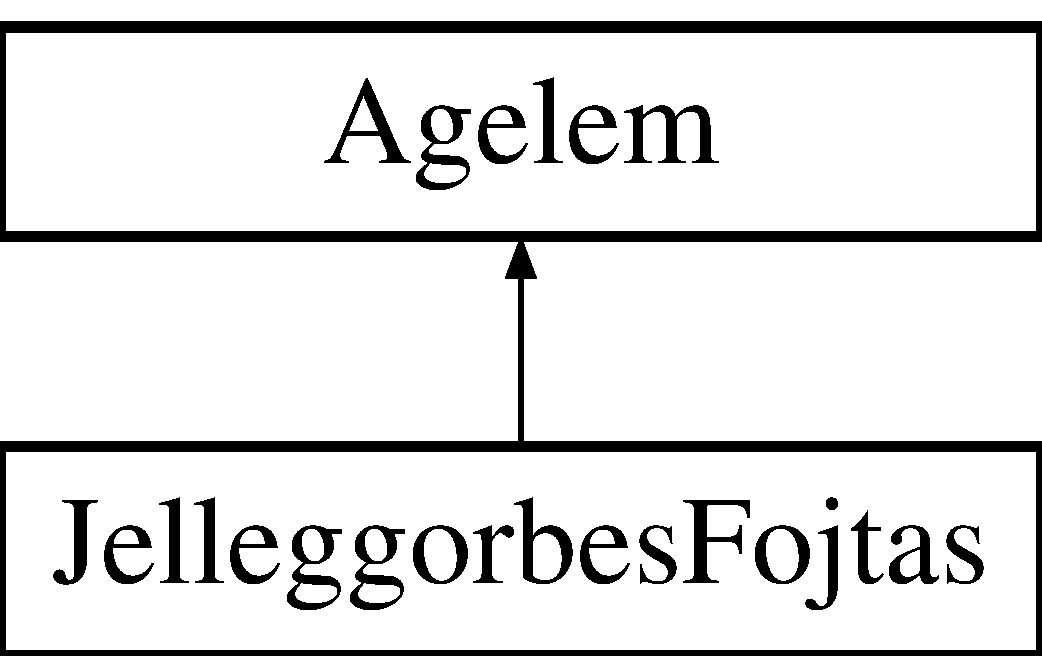
\includegraphics[height=2.000000cm]{class_jelleggorbes_fojtas}
\end{center}
\end{figure}
\subsection*{Public Member Functions}
\begin{DoxyCompactItemize}
\item 
\hypertarget{class_jelleggorbes_fojtas_af66a653a2838a2a5a9669ecfd7dc6a0b}{}\label{class_jelleggorbes_fojtas_af66a653a2838a2a5a9669ecfd7dc6a0b} 
{\bfseries Jelleggorbes\+Fojtas} (const string \hyperlink{class_agelem_abe92b7e3912367d5d1caf6b277ca0b7d}{nev}, const string a\+\_\+cspe\+\_\+nev, const string a\+\_\+cspv\+\_\+nev, const double a\+\_\+ro, const double \hyperlink{class_agelem_a3f8668febc2958fd539997d537552f17}{Aref}, const vector$<$ double $>$e, const vector$<$ double $>$ zeta, const double allas, const double a\+\_\+mp)
\item 
\hypertarget{class_jelleggorbes_fojtas_a8ac49ed546134b5147796be94b22521a}{}\label{class_jelleggorbes_fojtas_a8ac49ed546134b5147796be94b22521a} 
void {\bfseries Update\+\_\+zeta} ()
\item 
\hypertarget{class_jelleggorbes_fojtas_a86d24b2271e234200a7ecbdccd4e94c1}{}\label{class_jelleggorbes_fojtas_a86d24b2271e234200a7ecbdccd4e94c1} 
string \hyperlink{class_jelleggorbes_fojtas_a86d24b2271e234200a7ecbdccd4e94c1}{Info} ()
\begin{DoxyCompactList}\small\item\em Informacio. \end{DoxyCompactList}\item 
\hypertarget{class_jelleggorbes_fojtas_a86bd9df0aa43f56c29dd451c92368724}{}\label{class_jelleggorbes_fojtas_a86bd9df0aa43f56c29dd451c92368724} 
double \hyperlink{class_jelleggorbes_fojtas_a86bd9df0aa43f56c29dd451c92368724}{f} (vector$<$ double $>$)
\begin{DoxyCompactList}\small\item\em Az agegyenlet erteke, nullara rendezve, v.\+o.\+m.-\/ben. \end{DoxyCompactList}\item 
\hypertarget{class_jelleggorbes_fojtas_a4962bb9e88d9f4c6453f1e57ae3c2041}{}\label{class_jelleggorbes_fojtas_a4962bb9e88d9f4c6453f1e57ae3c2041} 
vector$<$ double $>$ \hyperlink{class_jelleggorbes_fojtas_a4962bb9e88d9f4c6453f1e57ae3c2041}{df} (vector$<$ double $>$)
\begin{DoxyCompactList}\small\item\em Jacobi\+: df/dhe, df/dhv, df/dmp, konstans tag. \end{DoxyCompactList}\item 
\hypertarget{class_jelleggorbes_fojtas_a6e095b972116dd9b3dd0635dbbd4edb9}{}\label{class_jelleggorbes_fojtas_a6e095b972116dd9b3dd0635dbbd4edb9} 
void \hyperlink{class_jelleggorbes_fojtas_a6e095b972116dd9b3dd0635dbbd4edb9}{Ini} (int mode, double value)
\begin{DoxyCompactList}\small\item\em Inicializacio, mode=0 -\/$>$ automatikus, mode=1 -\/$>$ value beirasa. \end{DoxyCompactList}\item 
\hypertarget{class_jelleggorbes_fojtas_a1af41ea01aa004c5c709fed5760f1de1}{}\label{class_jelleggorbes_fojtas_a1af41ea01aa004c5c709fed5760f1de1} 
void {\bfseries Set\+\_\+dprop} (string mit, double mire)
\item 
\hypertarget{class_jelleggorbes_fojtas_ab5e5487da5f674affde45438021c0967}{}\label{class_jelleggorbes_fojtas_ab5e5487da5f674affde45438021c0967} 
double \hyperlink{class_jelleggorbes_fojtas_ab5e5487da5f674affde45438021c0967}{Get\+\_\+dprop} (string mit)
\begin{DoxyCompactList}\small\item\em Get double property, \hyperlink{class_cso}{Cso} es \hyperlink{class_csatorna}{Csatorna} akarja elulirja. \end{DoxyCompactList}\item 
\hypertarget{class_jelleggorbes_fojtas_a99692fcbf4be938803671901230f11ae}{}\label{class_jelleggorbes_fojtas_a99692fcbf4be938803671901230f11ae} 
string {\bfseries Get\+Type} ()
\end{DoxyCompactItemize}
\subsection*{Additional Inherited Members}


The documentation for this class was generated from the following files\+:\begin{DoxyCompactItemize}
\item 
Jelleggorbes\+Fojtas.\+h\item 
Jelleggorbes\+Fojtas.\+cpp\end{DoxyCompactItemize}

\hypertarget{class_konst_nyomas}{}\section{Konst\+Nyomas Class Reference}
\label{class_konst_nyomas}\index{Konst\+Nyomas@{Konst\+Nyomas}}
Inheritance diagram for Konst\+Nyomas\+:\begin{figure}[H]
\begin{center}
\leavevmode
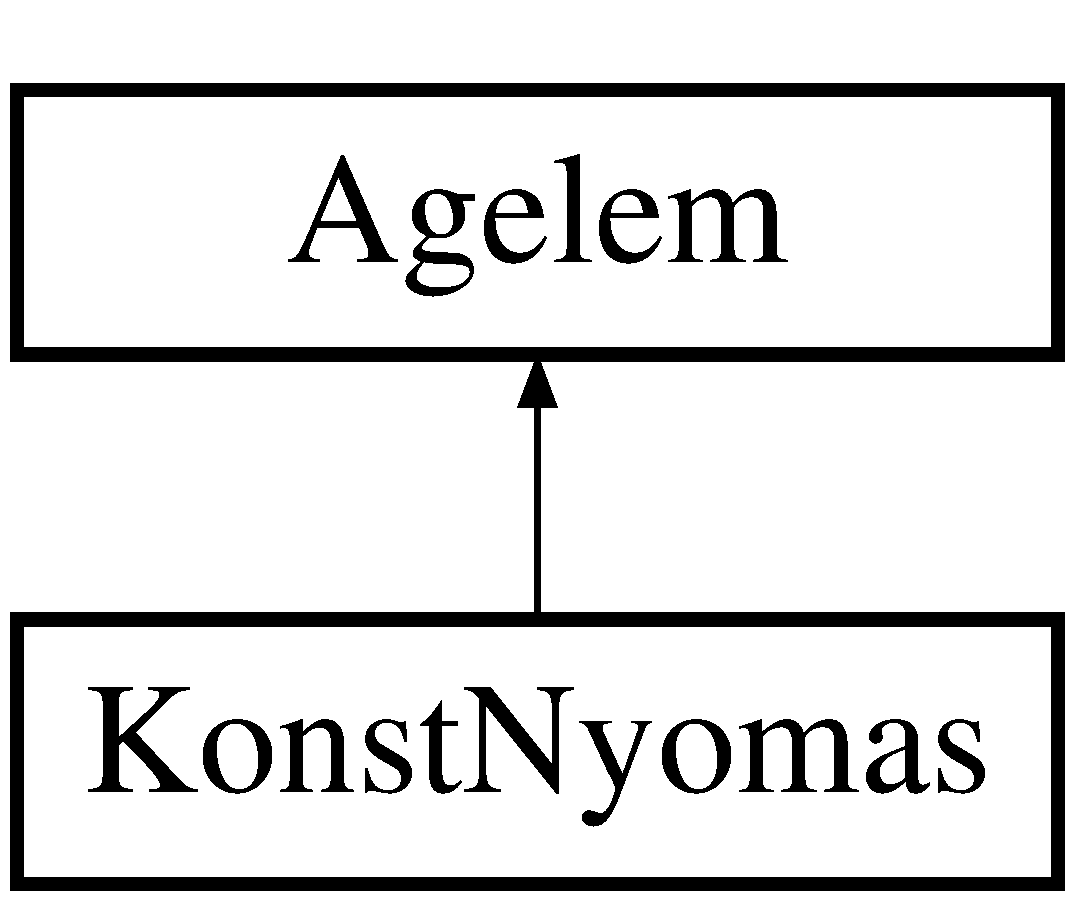
\includegraphics[height=2.000000cm]{class_konst_nyomas}
\end{center}
\end{figure}
\subsection*{Public Member Functions}
\begin{DoxyCompactItemize}
\item 
{\bfseries Konst\+Nyomas} (const string \hyperlink{class_agelem_abe92b7e3912367d5d1caf6b277ca0b7d}{nev}, const double \hyperlink{class_agelem_a3f8668febc2958fd539997d537552f17}{Aref}, const string cspnev, const double a\+\_\+ro, const double p, const double \hyperlink{class_agelem_a1377d80d8511cc4adacccba31d28282d}{mp}, const double tt)\hypertarget{class_konst_nyomas_a729b5f380b7ea5792484e963b1383f34}{}\label{class_konst_nyomas_a729b5f380b7ea5792484e963b1383f34}

\item 
string \hyperlink{class_konst_nyomas_a61f8d31204f60c216808fce1da451c30}{Info} ()\hypertarget{class_konst_nyomas_a61f8d31204f60c216808fce1da451c30}{}\label{class_konst_nyomas_a61f8d31204f60c216808fce1da451c30}

\begin{DoxyCompactList}\small\item\em Informacio. \end{DoxyCompactList}\item 
double \hyperlink{class_konst_nyomas_a71a45ebdb2f27a8f69b9988f8ac5f50c}{f} (vector$<$ double $>$)\hypertarget{class_konst_nyomas_a71a45ebdb2f27a8f69b9988f8ac5f50c}{}\label{class_konst_nyomas_a71a45ebdb2f27a8f69b9988f8ac5f50c}

\begin{DoxyCompactList}\small\item\em Az agegyenlet erteke, nullara rendezve, v.\+o.\+m.-\/ben. \end{DoxyCompactList}\item 
vector$<$ double $>$ \hyperlink{class_konst_nyomas_ab8b056adc0788048a2b32f5378ef07b4}{df} (vector$<$ double $>$)\hypertarget{class_konst_nyomas_ab8b056adc0788048a2b32f5378ef07b4}{}\label{class_konst_nyomas_ab8b056adc0788048a2b32f5378ef07b4}

\begin{DoxyCompactList}\small\item\em Jacobi\+: df/dhe, df/dhv, df/dmp, konstans tag. \end{DoxyCompactList}\item 
void \hyperlink{class_konst_nyomas_a9f949a7c2430ade86328f9f0c5189797}{Ini} (int mode, double value)\hypertarget{class_konst_nyomas_a9f949a7c2430ade86328f9f0c5189797}{}\label{class_konst_nyomas_a9f949a7c2430ade86328f9f0c5189797}

\begin{DoxyCompactList}\small\item\em Inicializacio, mode=0 -\/$>$ automatikus, mode=1 -\/$>$ value beirasa. \end{DoxyCompactList}\item 
void {\bfseries Set\+\_\+dprop} (string mit, double mire)\hypertarget{class_konst_nyomas_aebe3ac3a8be035145dbc56429c8d2831}{}\label{class_konst_nyomas_aebe3ac3a8be035145dbc56429c8d2831}

\item 
string {\bfseries Get\+Type} ()\hypertarget{class_konst_nyomas_ac142568860665970fab5de0921758f2e}{}\label{class_konst_nyomas_ac142568860665970fab5de0921758f2e}

\end{DoxyCompactItemize}
\subsection*{Additional Inherited Members}


The documentation for this class was generated from the following files\+:\begin{DoxyCompactItemize}
\item 
Konst\+Nyomas.\+h\item 
Konst\+Nyomas.\+cpp\end{DoxyCompactItemize}

\hypertarget{struct_next_token}{}\section{Next\+Token Struct Reference}
\label{struct_next_token}\index{Next\+Token@{Next\+Token}}
\subsection*{Public Attributes}
\begin{DoxyCompactItemize}
\item 
\mbox{\Hypertarget{struct_next_token_abdf8ae1822a48d9d753cef22974b661a}\label{struct_next_token_abdf8ae1822a48d9d753cef22974b661a}} 
\hyperlink{struct_a_l_l_x_m_l_clear_tag}{A\+L\+L\+X\+M\+L\+Clear\+Tag} $\ast$ {\bfseries p\+Clr}
\item 
\mbox{\Hypertarget{struct_next_token_a235b34c915ba7bba132d9f166af6ab37}\label{struct_next_token_a235b34c915ba7bba132d9f166af6ab37}} 
X\+M\+L\+C\+S\+TR {\bfseries p\+Str}
\end{DoxyCompactItemize}


The documentation for this struct was generated from the following file\+:\begin{DoxyCompactItemize}
\item 
xml\+Parser.\+cpp\end{DoxyCompactItemize}

\hypertarget{class_n_r_mat}{}\section{N\+R\+Mat$<$ T $>$ Class Template Reference}
\label{class_n_r_mat}\index{N\+R\+Mat$<$ T $>$@{N\+R\+Mat$<$ T $>$}}
\subsection*{Public Member Functions}
\begin{DoxyCompactItemize}
\item 
\mbox{\Hypertarget{class_n_r_mat_a1110d5f3fb74e69a0a06e0873e0dfb8c}\label{class_n_r_mat_a1110d5f3fb74e69a0a06e0873e0dfb8c}} 
{\bfseries N\+R\+Mat} (int n, int m)
\item 
\mbox{\Hypertarget{class_n_r_mat_ab7e5747ce28ec13e19885907cdac60f4}\label{class_n_r_mat_ab7e5747ce28ec13e19885907cdac60f4}} 
{\bfseries N\+R\+Mat} (const T \&a, int n, int m)
\item 
\mbox{\Hypertarget{class_n_r_mat_a223fc0d7bfb1a12e48b87072034d3912}\label{class_n_r_mat_a223fc0d7bfb1a12e48b87072034d3912}} 
{\bfseries N\+R\+Mat} (const T $\ast$a, int n, int m)
\item 
\mbox{\Hypertarget{class_n_r_mat_a5a99f340753f4791a31de756ad1e3524}\label{class_n_r_mat_a5a99f340753f4791a31de756ad1e3524}} 
{\bfseries N\+R\+Mat} (const \hyperlink{class_n_r_mat}{N\+R\+Mat} \&rhs)
\item 
\mbox{\Hypertarget{class_n_r_mat_a83b7a22bc216f3b75aca356b077d3eb0}\label{class_n_r_mat_a83b7a22bc216f3b75aca356b077d3eb0}} 
\hyperlink{class_n_r_mat}{N\+R\+Mat} \& {\bfseries operator=} (const \hyperlink{class_n_r_mat}{N\+R\+Mat} \&rhs)
\item 
\mbox{\Hypertarget{class_n_r_mat_a5c0ef740d322d4a8a6b21d4da1053e2f}\label{class_n_r_mat_a5c0ef740d322d4a8a6b21d4da1053e2f}} 
\hyperlink{class_n_r_mat}{N\+R\+Mat} \& {\bfseries operator=} (const T \&a)
\item 
\mbox{\Hypertarget{class_n_r_mat_a947ff7588b1eed80fed633e8b001838b}\label{class_n_r_mat_a947ff7588b1eed80fed633e8b001838b}} 
T $\ast$ {\bfseries operator\mbox{[}$\,$\mbox{]}} (const int i)
\item 
\mbox{\Hypertarget{class_n_r_mat_a8ae8abcf7c56932b621a90f7898131c4}\label{class_n_r_mat_a8ae8abcf7c56932b621a90f7898131c4}} 
const T $\ast$ {\bfseries operator\mbox{[}$\,$\mbox{]}} (const int i) const
\item 
\mbox{\Hypertarget{class_n_r_mat_a10475233c8657903b0e07e9b26711c99}\label{class_n_r_mat_a10475233c8657903b0e07e9b26711c99}} 
int {\bfseries nrows} () const
\item 
\mbox{\Hypertarget{class_n_r_mat_a40a975f0eb93b836904b0027a316932e}\label{class_n_r_mat_a40a975f0eb93b836904b0027a316932e}} 
int {\bfseries ncols} () const
\end{DoxyCompactItemize}


The documentation for this class was generated from the following file\+:\begin{DoxyCompactItemize}
\item 
nrutil\+\_\+nr.\+h\end{DoxyCompactItemize}

\hypertarget{class_n_r_mat3d}{}\section{N\+R\+Mat3d$<$ T $>$ Class Template Reference}
\label{class_n_r_mat3d}\index{N\+R\+Mat3d$<$ T $>$@{N\+R\+Mat3d$<$ T $>$}}
\subsection*{Public Member Functions}
\begin{DoxyCompactItemize}
\item 
\hypertarget{class_n_r_mat3d_ac98efbf6768cfde88627dce5bb4f001e}{}\label{class_n_r_mat3d_ac98efbf6768cfde88627dce5bb4f001e} 
{\bfseries N\+R\+Mat3d} (int n, int m, int k)
\item 
\hypertarget{class_n_r_mat3d_a2b9bc9432bb004531a413ce6fcc251cf}{}\label{class_n_r_mat3d_a2b9bc9432bb004531a413ce6fcc251cf} 
T $\ast$$\ast$ {\bfseries operator\mbox{[}$\,$\mbox{]}} (const int i)
\item 
\hypertarget{class_n_r_mat3d_a548d5562235bbbd8a706a8b88c206934}{}\label{class_n_r_mat3d_a548d5562235bbbd8a706a8b88c206934} 
const T $\ast$const  $\ast$ {\bfseries operator\mbox{[}$\,$\mbox{]}} (const int i) const
\item 
\hypertarget{class_n_r_mat3d_a6acacd12a0a559a4d083c9c4124d93b5}{}\label{class_n_r_mat3d_a6acacd12a0a559a4d083c9c4124d93b5} 
int {\bfseries dim1} () const
\item 
\hypertarget{class_n_r_mat3d_acee8beead1af530aee40cef27aa9ffc1}{}\label{class_n_r_mat3d_acee8beead1af530aee40cef27aa9ffc1} 
int {\bfseries dim2} () const
\item 
\hypertarget{class_n_r_mat3d_a857ac41bd02ab1d4b11e1522238b03e9}{}\label{class_n_r_mat3d_a857ac41bd02ab1d4b11e1522238b03e9} 
int {\bfseries dim3} () const
\end{DoxyCompactItemize}


The documentation for this class was generated from the following file\+:\begin{DoxyCompactItemize}
\item 
nrutil\+\_\+nr.\+h\end{DoxyCompactItemize}

\hypertarget{class_n_r_vec}{}\section{N\+R\+Vec$<$ T $>$ Class Template Reference}
\label{class_n_r_vec}\index{N\+R\+Vec$<$ T $>$@{N\+R\+Vec$<$ T $>$}}
\subsection*{Public Member Functions}
\begin{DoxyCompactItemize}
\item 
{\bfseries N\+R\+Vec} (int n)\hypertarget{class_n_r_vec_a478e724d382133add68eb125d7d32902}{}\label{class_n_r_vec_a478e724d382133add68eb125d7d32902}

\item 
{\bfseries N\+R\+Vec} (const T \&a, int n)\hypertarget{class_n_r_vec_a8e7741f242e11d33fedf292b92aeed12}{}\label{class_n_r_vec_a8e7741f242e11d33fedf292b92aeed12}

\item 
{\bfseries N\+R\+Vec} (const T $\ast$a, int n)\hypertarget{class_n_r_vec_af1017a82c93d1b000b7b6c220d62ffd3}{}\label{class_n_r_vec_af1017a82c93d1b000b7b6c220d62ffd3}

\item 
{\bfseries N\+R\+Vec} (const \hyperlink{class_n_r_vec}{N\+R\+Vec} \&rhs)\hypertarget{class_n_r_vec_a9d0c1a68537a31cf49ef8db9bf2b5d9e}{}\label{class_n_r_vec_a9d0c1a68537a31cf49ef8db9bf2b5d9e}

\item 
\hyperlink{class_n_r_vec}{N\+R\+Vec} \& {\bfseries operator=} (const \hyperlink{class_n_r_vec}{N\+R\+Vec} \&rhs)\hypertarget{class_n_r_vec_ab08c859a363e808089e50fd36a26c0b5}{}\label{class_n_r_vec_ab08c859a363e808089e50fd36a26c0b5}

\item 
\hyperlink{class_n_r_vec}{N\+R\+Vec} \& {\bfseries operator=} (const T \&a)\hypertarget{class_n_r_vec_ae6789b5563959a769c1abc7a4a710fe4}{}\label{class_n_r_vec_ae6789b5563959a769c1abc7a4a710fe4}

\item 
T \& {\bfseries operator\mbox{[}$\,$\mbox{]}} (const int i)\hypertarget{class_n_r_vec_a673ade054b9796afa0cac87636a3d1a6}{}\label{class_n_r_vec_a673ade054b9796afa0cac87636a3d1a6}

\item 
const T \& {\bfseries operator\mbox{[}$\,$\mbox{]}} (const int i) const \hypertarget{class_n_r_vec_aeb68c34fa9fa72c401708c12b130fafc}{}\label{class_n_r_vec_aeb68c34fa9fa72c401708c12b130fafc}

\item 
int {\bfseries size} () const \hypertarget{class_n_r_vec_acf12ca39695688c3d28faf8f58ea5d3b}{}\label{class_n_r_vec_acf12ca39695688c3d28faf8f58ea5d3b}

\end{DoxyCompactItemize}


The documentation for this class was generated from the following file\+:\begin{DoxyCompactItemize}
\item 
nrutil\+\_\+nr.\+h\end{DoxyCompactItemize}

\hypertarget{class_staci}{}\section{Staci Class Reference}
\label{class_staci}\index{Staci@{Staci}}
\subsection*{Public Member Functions}
\begin{DoxyCompactItemize}
\item 
\mbox{\Hypertarget{class_staci_ac0b3fc6ab6ed135b47b004e0053b51a1}\label{class_staci_ac0b3fc6ab6ed135b47b004e0053b51a1}} 
void {\bfseries export\+\_\+connected\+\_\+nodes} ()
\item 
\mbox{\Hypertarget{class_staci_a6f7ee7b08cba6b9a84a2472610fc9b30}\label{class_staci_a6f7ee7b08cba6b9a84a2472610fc9b30}} 
{\bfseries Staci} (int argc, char $\ast$argv\mbox{[}$\,$\mbox{]})
\item 
\mbox{\Hypertarget{class_staci_ae470e416c7900fe47a198deb48faa173}\label{class_staci_ae470e416c7900fe47a198deb48faa173}} 
{\bfseries Staci} (string spr\+\_\+filename)
\item 
\mbox{\Hypertarget{class_staci_a3b63425864b8bbc369a64e61803fe5fe}\label{class_staci_a3b63425864b8bbc369a64e61803fe5fe}} 
string {\bfseries Get\+\_\+out\+\_\+file} ()
\item 
\mbox{\Hypertarget{class_staci_a60eb2cc5e192ece5607684d13252ea42}\label{class_staci_a60eb2cc5e192ece5607684d13252ea42}} 
int {\bfseries Get\+\_\+debug\+\_\+level} ()
\item 
\mbox{\Hypertarget{class_staci_aae5279dcb5e5ac4543aa1bcf0b104da1}\label{class_staci_aae5279dcb5e5ac4543aa1bcf0b104da1}} 
void {\bfseries Set\+\_\+debug\+\_\+level} (int a\+\_\+debug\+\_\+level)
\item 
\mbox{\Hypertarget{class_staci_a0153c20898e554922b15cee551a9f982}\label{class_staci_a0153c20898e554922b15cee551a9f982}} 
void {\bfseries build\+\_\+system} ()
\item 
\mbox{\Hypertarget{class_staci_ac8690e5b15e90589d09bf72b07d24e5e}\label{class_staci_ac8690e5b15e90589d09bf72b07d24e5e}} 
void {\bfseries build\+\_\+system\+\_\+old} ()
\item 
\mbox{\Hypertarget{class_staci_ad884bf7a487813b79d2a171cbfd0537a}\label{class_staci_ad884bf7a487813b79d2a171cbfd0537a}} 
void {\bfseries ini} ()
\item 
\mbox{\Hypertarget{class_staci_ad52e09f1b75b48551ce5fbc8aad042cc}\label{class_staci_ad52e09f1b75b48551ce5fbc8aad042cc}} 
void {\bfseries ini} (const \hyperlink{class_staci}{Staci} $\ast$Ini\+Staci)
\item 
\mbox{\Hypertarget{class_staci_ae95917401c8454a747a24880faa20138}\label{class_staci_ae95917401c8454a747a24880faa20138}} 
void {\bfseries list\+\_\+system} ()
\item 
\mbox{\Hypertarget{class_staci_a54bf8a354a57dbafda0bf775c66d6524}\label{class_staci_a54bf8a354a57dbafda0bf775c66d6524}} 
string {\bfseries list\+\_\+results} ()
\item 
\mbox{\Hypertarget{class_staci_a0cf78089da2693f039b4fe5e2b5c21d2}\label{class_staci_a0cf78089da2693f039b4fe5e2b5c21d2}} 
void {\bfseries save\+\_\+results} (bool conv\+\_\+reached)
\item 
\mbox{\Hypertarget{class_staci_a42bac4458094c023bc91dcb9ccf4a029}\label{class_staci_a42bac4458094c023bc91dcb9ccf4a029}} 
void {\bfseries save\+\_\+mod\+\_\+prop} (bool is\+\_\+general\+\_\+property)
\item 
\mbox{\Hypertarget{class_staci_a232a3767e1039491a83690f564702089}\label{class_staci_a232a3767e1039491a83690f564702089}} 
void {\bfseries save\+\_\+mod\+\_\+prop\+\_\+all\+\_\+elements} (string property\+\_\+\+ID)
\item 
\mbox{\Hypertarget{class_staci_a86917fe19f9c274dac7fbf5fd86e44ba}\label{class_staci_a86917fe19f9c274dac7fbf5fd86e44ba}} 
bool {\bfseries solve\+\_\+system} ()
\item 
\mbox{\Hypertarget{class_staci_a884616aaebef6a088c562e56c0f68525}\label{class_staci_a884616aaebef6a088c562e56c0f68525}} 
void {\bfseries solve\+\_\+residence\+\_\+time} ()
\item 
\mbox{\Hypertarget{class_staci_a403aabb120769ddc037a69548b2c2134}\label{class_staci_a403aabb120769ddc037a69548b2c2134}} 
void {\bfseries residence\+\_\+time\+\_\+step} (string \&max\+\_\+\+ID, double \&max\+\_\+\+V\+AL, double \&mean\+\_\+\+V\+AL)
\item 
\mbox{\Hypertarget{class_staci_ad9b04218bcc23ddc5b6e1d247f5ffb8f}\label{class_staci_ad9b04218bcc23ddc5b6e1d247f5ffb8f}} 
bool {\bfseries solve\+\_\+system\+\_\+old} ()
\item 
\mbox{\Hypertarget{class_staci_ac71d40c423576c540b594c7e3a7f1365}\label{class_staci_ac71d40c423576c540b594c7e3a7f1365}} 
void {\bfseries set\+\_\+up\+\_\+transport} ()
\item 
\mbox{\Hypertarget{class_staci_a8ac839cd977519ad3a6a6a5ba85f4d35}\label{class_staci_a8ac839cd977519ad3a6a6a5ba85f4d35}} 
void {\bfseries solve\+\_\+transport} (int mode)
\item 
\mbox{\Hypertarget{class_staci_a7dde80c0f00d33639f459fca9d7b1314}\label{class_staci_a7dde80c0f00d33639f459fca9d7b1314}} 
double {\bfseries get\+\_\+oldest} ()
\item 
\mbox{\Hypertarget{class_staci_a82c116ba2e4338362e1efa7410acba07}\label{class_staci_a82c116ba2e4338362e1efa7410acba07}} 
void {\bfseries transport\+\_\+step} (double dt)
\item 
\mbox{\Hypertarget{class_staci_a2ae0957cb2159f7417175379bac09d95}\label{class_staci_a2ae0957cb2159f7417175379bac09d95}} 
double {\bfseries teta} (double c, const int i)
\item 
\mbox{\Hypertarget{class_staci_a7c79de7b27f86ef08e48eef757e895fa}\label{class_staci_a7c79de7b27f86ef08e48eef757e895fa}} 
void {\bfseries export\+\_\+to\+\_\+aisee} ()
\item 
\mbox{\Hypertarget{class_staci_ac0af3f19c34f3a08e4892cebdc5e0340}\label{class_staci_ac0af3f19c34f3a08e4892cebdc5e0340}} 
void {\bfseries post\+\_\+process\+\_\+res\+\_\+file} ()
\item 
\mbox{\Hypertarget{class_staci_af0d4816a00fec9373f469a7854f09a0e}\label{class_staci_af0d4816a00fec9373f469a7854f09a0e}} 
void {\bfseries logfile\+\_\+write} (string msg, int msg\+\_\+debug\+\_\+level)
\item 
\mbox{\Hypertarget{class_staci_a03c12265bef1640238ffe1efdb0a2556}\label{class_staci_a03c12265bef1640238ffe1efdb0a2556}} 
void {\bfseries set\+\_\+res\+\_\+file} (string xml\+\_\+fnev)
\item 
\mbox{\Hypertarget{class_staci_a2939f5a02b2d06e21be553d31a15106c}\label{class_staci_a2939f5a02b2d06e21be553d31a15106c}} 
void {\bfseries set\+\_\+ini\+\_\+file} (string xml\+\_\+fnev)
\item 
\mbox{\Hypertarget{class_staci_a80220c0c3baa490866bd2fc15698a8d1}\label{class_staci_a80220c0c3baa490866bd2fc15698a8d1}} 
void {\bfseries set\+\_\+out\+\_\+file} (string fnev)
\item 
\mbox{\Hypertarget{class_staci_a00500602fabd3f2cdc0bd7fedc845787}\label{class_staci_a00500602fabd3f2cdc0bd7fedc845787}} 
void {\bfseries set\+\_\+progress\+\_\+file} (string fnev)
\item 
\mbox{\Hypertarget{class_staci_a61dc8ef1b4e1561938e6cc39917b346f}\label{class_staci_a61dc8ef1b4e1561938e6cc39917b346f}} 
string {\bfseries get\+\_\+def\+\_\+file} ()
\item 
\mbox{\Hypertarget{class_staci_a0c822a9effbcf4dd88b82f68b38c0498}\label{class_staci_a0c822a9effbcf4dd88b82f68b38c0498}} 
int {\bfseries get\+\_\+mode} ()
\item 
\mbox{\Hypertarget{class_staci_a9c1d34d2dc05eaad3c5ba60d5ebfa5a1}\label{class_staci_a9c1d34d2dc05eaad3c5ba60d5ebfa5a1}} 
void {\bfseries save\+\_\+transport} (int mode)
\item 
\mbox{\Hypertarget{class_staci_ac38df6cb7fb51eb595c17cd050a85073}\label{class_staci_ac38df6cb7fb51eb595c17cd050a85073}} 
void {\bfseries copy\+\_\+file} (const string in\+\_\+f\+\_\+nev, const string out\+\_\+f\+\_\+nev)
\item 
\mbox{\Hypertarget{class_staci_a0f2f821b672c0aa1a2f9a9117c2f67ef}\label{class_staci_a0f2f821b672c0aa1a2f9a9117c2f67ef}} 
void {\bfseries set\+\_\+van\+\_\+ini} (const bool van\+\_\+e)
\item 
\mbox{\Hypertarget{class_staci_ae13ac77f30c2f64ffbc44e9b271373ef}\label{class_staci_ae13ac77f30c2f64ffbc44e9b271373ef}} 
void {\bfseries Set\+\_\+\+Foly\+Terf} ()
\item 
\mbox{\Hypertarget{class_staci_a292d7cba265ab37d31bec35349fae1ac}\label{class_staci_a292d7cba265ab37d31bec35349fae1ac}} 
double {\bfseries m\+\_\+get\+\_\+dprop} ()
\item 
\mbox{\Hypertarget{class_staci_a47fc932a04e285791a4cb4227e840004}\label{class_staci_a47fc932a04e285791a4cb4227e840004}} 
void {\bfseries m\+\_\+set\+\_\+dprop} ()
\item 
\mbox{\Hypertarget{class_staci_af333518d7badd70d8ae324c0287a94e0}\label{class_staci_af333518d7badd70d8ae324c0287a94e0}} 
double {\bfseries get\+\_\+dprop} (string ID, string prop)
\item 
\mbox{\Hypertarget{class_staci_a1028b9dd75388d7d3e42d10b31a9e6eb}\label{class_staci_a1028b9dd75388d7d3e42d10b31a9e6eb}} 
void {\bfseries set\+\_\+dprop} (string ID, string prop, double val)
\item 
\mbox{\Hypertarget{class_staci_a690304659f0bf2283a4e5dc20177661f}\label{class_staci_a690304659f0bf2283a4e5dc20177661f}} 
void {\bfseries list\+\_\+all\+\_\+elements} ()
\item 
\mbox{\Hypertarget{class_staci_a4f664e6fe326b5592664b2b7239612f2}\label{class_staci_a4f664e6fe326b5592664b2b7239612f2}} 
void {\bfseries Print\+\_\+\+Jacobian} ()
\item 
\mbox{\Hypertarget{class_staci_abe8ddaf47c48ac2429acc5fe9c8010a5}\label{class_staci_abe8ddaf47c48ac2429acc5fe9c8010a5}} 
void {\bfseries Print\+\_\+dfdmu} ()
\item 
\mbox{\Hypertarget{class_staci_ac3b009354096542602b5a6849f5114d2}\label{class_staci_ac3b009354096542602b5a6849f5114d2}} 
void {\bfseries Print\+\_\+dxdmu} ()
\item 
\mbox{\Hypertarget{class_staci_abf31b6f78c548e42970b98941d35aba9}\label{class_staci_abf31b6f78c548e42970b98941d35aba9}} 
void {\bfseries Compute\+\_\+dxdmu} ()
\item 
\mbox{\Hypertarget{class_staci_afc29a7cbf16da192dfdece5f689546e5}\label{class_staci_afc29a7cbf16da192dfdece5f689546e5}} 
void {\bfseries Compute\+\_\+\+Sensitivity\+\_\+\+Matrix} (string parameter, int scale)
\item 
void \hyperlink{class_staci_adfa2f37ff32dedbb4f71df48951ed786}{Save\+\_\+\+Sensitivity} ()
\item 
\mbox{\Hypertarget{class_staci_a981510ebb2cb58d898fb258063d6f890}\label{class_staci_a981510ebb2cb58d898fb258063d6f890}} 
void {\bfseries set\+\_\+do\+\_\+save\+\_\+file} (const bool save\+\_\+it)
\item 
\mbox{\Hypertarget{class_staci_a920547ca1fbf6da0fe4b80db05a5e027}\label{class_staci_a920547ca1fbf6da0fe4b80db05a5e027}} 
double {\bfseries get\+\_\+sum\+\_\+of\+\_\+consumption} ()
\item 
\mbox{\Hypertarget{class_staci_a382120835654d66e09b2975b22809b76}\label{class_staci_a382120835654d66e09b2975b22809b76}} 
double {\bfseries get\+\_\+sum\+\_\+of\+\_\+pos\+\_\+consumption} ()
\item 
\mbox{\Hypertarget{class_staci_a00fff9cdb062d4101604e5cb0ffa673c}\label{class_staci_a00fff9cdb062d4101604e5cb0ffa673c}} 
double {\bfseries get\+\_\+sum\+\_\+of\+\_\+neg\+\_\+consumption} ()
\item 
\mbox{\Hypertarget{class_staci_a93e861cc624e16e4fe897c4cc88ac729}\label{class_staci_a93e861cc624e16e4fe897c4cc88ac729}} 
double {\bfseries Get\+Min\+Pipe\+Diameter} (int \&idx)
\item 
\mbox{\Hypertarget{class_staci_a8cdd05ac08ee1b6efe3fe0094d502ce1}\label{class_staci_a8cdd05ac08ee1b6efe3fe0094d502ce1}} 
double {\bfseries Get\+Max\+Pipe\+Diameter} (int \&idx)
\item 
\mbox{\Hypertarget{class_staci_ae48a8e0de1ac049d9b91d9d91aa3f853}\label{class_staci_ae48a8e0de1ac049d9b91d9d91aa3f853}} 
double {\bfseries Get\+Min\+Pipe\+Length} (int \&idx)
\item 
\mbox{\Hypertarget{class_staci_a1ac3bd68b82e31098889d8cc7079fa23}\label{class_staci_a1ac3bd68b82e31098889d8cc7079fa23}} 
double {\bfseries Get\+Max\+Pipe\+Length} (int \&idx)
\item 
\mbox{\Hypertarget{class_staci_a639a97b58a3b190b8e408525d08b1d5a}\label{class_staci_a639a97b58a3b190b8e408525d08b1d5a}} 
double {\bfseries Get\+Sum\+Pipe\+Length} ()
\item 
\mbox{\Hypertarget{class_staci_a33cc0e549bf466f5613c2234430ddbc1}\label{class_staci_a33cc0e549bf466f5613c2234430ddbc1}} 
double {\bfseries Get\+Sum\+Pipe\+Volume} ()
\item 
\mbox{\Hypertarget{class_staci_a4ffa8fbe32cb738b3aa6223ecd1d34eb}\label{class_staci_a4ffa8fbe32cb738b3aa6223ecd1d34eb}} 
double {\bfseries Get\+Min\+Consumption} (int \&idx)
\item 
\mbox{\Hypertarget{class_staci_a67d661c84d23d50b78eadaac79648fb1}\label{class_staci_a67d661c84d23d50b78eadaac79648fb1}} 
double {\bfseries Get\+Max\+Consumption} (int \&idx)
\item 
\mbox{\Hypertarget{class_staci_a6f0b1ea987db6898b02fb0b5ee81c08a}\label{class_staci_a6f0b1ea987db6898b02fb0b5ee81c08a}} 
double {\bfseries Get\+Min\+Geo\+Height} (int \&idx)
\item 
\mbox{\Hypertarget{class_staci_a6698b72588fe59909594948920f16e4e}\label{class_staci_a6698b72588fe59909594948920f16e4e}} 
double {\bfseries Get\+Max\+Geo\+Height} (int \&idx)
\item 
\mbox{\Hypertarget{class_staci_a185f2c986890fbde90693c7133492b04}\label{class_staci_a185f2c986890fbde90693c7133492b04}} 
void {\bfseries Statistics} ()
\end{DoxyCompactItemize}
\subsection*{Public Attributes}
\begin{DoxyCompactItemize}
\item 
\mbox{\Hypertarget{class_staci_a1b5c85269be922a1ed62890cd88e67db}\label{class_staci_a1b5c85269be922a1ed62890cd88e67db}} 
vector$<$ \hyperlink{class_csomopont}{Csomopont} $\ast$ $>$ {\bfseries cspok}
\item 
\mbox{\Hypertarget{class_staci_a6ca23dec6bf9e864efe535d836b7d02d}\label{class_staci_a6ca23dec6bf9e864efe535d836b7d02d}} 
vector$<$ \hyperlink{class_agelem}{Agelem} $\ast$ $>$ {\bfseries agelemek}
\item 
\mbox{\Hypertarget{class_staci_a23892863b8dba7d6493cbf474042f900}\label{class_staci_a23892863b8dba7d6493cbf474042f900}} 
double {\bfseries tt\+\_\+length}
\item 
\mbox{\Hypertarget{class_staci_acaa2f299629d12a61ab95b8522ef291a}\label{class_staci_acaa2f299629d12a61ab95b8522ef291a}} 
double {\bfseries cl\+\_\+length}
\item 
\mbox{\Hypertarget{class_staci_a2b3fec06ed59e026c2c34b7f82bf32e7}\label{class_staci_a2b3fec06ed59e026c2c34b7f82bf32e7}} 
string {\bfseries new\+\_\+def\+\_\+file}
\item 
\mbox{\Hypertarget{class_staci_a257ffac68d249e9ad21b982b8ea995c5}\label{class_staci_a257ffac68d249e9ad21b982b8ea995c5}} 
string {\bfseries element\+\_\+\+ID}
\item 
\mbox{\Hypertarget{class_staci_a9978fa86e2702420213256cd41e5de39}\label{class_staci_a9978fa86e2702420213256cd41e5de39}} 
string {\bfseries property\+\_\+\+ID}
\item 
\mbox{\Hypertarget{class_staci_a52df2bacb03971d6b49f28b5d57d8db5}\label{class_staci_a52df2bacb03971d6b49f28b5d57d8db5}} 
double {\bfseries new\+Value}
\item 
\mbox{\Hypertarget{class_staci_aa4c3b6e4e9c54ab81cfb9e33ad2b26f8}\label{class_staci_aa4c3b6e4e9c54ab81cfb9e33ad2b26f8}} 
vector$<$ vector$<$ double $>$ $>$ {\bfseries S\+M\+\_\+\+Mass\+Flow\+Rates}
\item 
\mbox{\Hypertarget{class_staci_a9e91205defa3e90dbfb6e93e229d3ee2}\label{class_staci_a9e91205defa3e90dbfb6e93e229d3ee2}} 
vector$<$ vector$<$ double $>$ $>$ {\bfseries S\+M\+\_\+\+Pressures}
\item 
\mbox{\Hypertarget{class_staci_ae5c1647a9b240fbcd91a684570c422e5}\label{class_staci_ae5c1647a9b240fbcd91a684570c422e5}} 
vector$<$ string $>$ {\bfseries S\+M\+\_\+row\+\_\+name}
\item 
\mbox{\Hypertarget{class_staci_a7b12823f45158095f1dada4da44196a5}\label{class_staci_a7b12823f45158095f1dada4da44196a5}} 
vector$<$ double $>$ {\bfseries S\+M\+\_\+row\+\_\+sum\+\_\+\+Mass\+Flow\+Rates}
\item 
\mbox{\Hypertarget{class_staci_a3583d4f48a560fc7d690ce23bf2a0b99}\label{class_staci_a3583d4f48a560fc7d690ce23bf2a0b99}} 
vector$<$ double $>$ {\bfseries S\+M\+\_\+row\+\_\+sum\+\_\+\+Pressures}
\item 
\mbox{\Hypertarget{class_staci_a65be5fdc061a8b906b12758fae210cef}\label{class_staci_a65be5fdc061a8b906b12758fae210cef}} 
vector$<$ string $>$ {\bfseries S\+M\+\_\+col\+\_\+name}
\item 
\mbox{\Hypertarget{class_staci_a88c1be986fb791fc2d6dcf188e492ee4}\label{class_staci_a88c1be986fb791fc2d6dcf188e492ee4}} 
vector$<$ double $>$ {\bfseries S\+M\+\_\+col\+\_\+sum\+\_\+\+Mass\+Flow\+Rates}
\item 
\mbox{\Hypertarget{class_staci_af7abda3370dc818d72e570aa2f5e9225}\label{class_staci_af7abda3370dc818d72e570aa2f5e9225}} 
vector$<$ double $>$ {\bfseries S\+M\+\_\+col\+\_\+sum\+\_\+\+Pressures}
\end{DoxyCompactItemize}


\subsection{Member Function Documentation}
\mbox{\Hypertarget{class_staci_adfa2f37ff32dedbb4f71df48951ed786}\label{class_staci_adfa2f37ff32dedbb4f71df48951ed786}} 
\index{Staci@{Staci}!Save\+\_\+\+Sensitivity@{Save\+\_\+\+Sensitivity}}
\index{Save\+\_\+\+Sensitivity@{Save\+\_\+\+Sensitivity}!Staci@{Staci}}
\subsubsection{\texorpdfstring{Save\+\_\+\+Sensitivity()}{Save\_Sensitivity()}}
{\footnotesize\ttfamily void Staci\+::\+Save\+\_\+\+Sensitivity (\begin{DoxyParamCaption}{ }\end{DoxyParamCaption})}

\begin{DoxyRefDesc}{Todo}
\item[\hyperlink{todo__todo000001}{Todo}]Sensitivity is flushed to $<$concentration$>$\end{DoxyRefDesc}


A $<$tag$>$ must be created to be used for sensitivity information in the data file.

The documentation for this class was generated from the following files\+:\begin{DoxyCompactItemize}
\item 
Staci.\+h\item 
Staci.\+cpp\end{DoxyCompactItemize}

\hypertarget{class_staci_exception}{}\section{Staci\+Exception Class Reference}
\label{class_staci_exception}\index{Staci\+Exception@{Staci\+Exception}}
\subsection*{Public Member Functions}
\begin{DoxyCompactItemize}
\item 
\hypertarget{class_staci_exception_ac441a4dfe2feec55d6998c6adcf7deed}{}\label{class_staci_exception_ac441a4dfe2feec55d6998c6adcf7deed} 
{\bfseries Staci\+Exception} (string d)
\item 
\hypertarget{class_staci_exception_a125f36e7bcc2ce25386c8d41bab89640}{}\label{class_staci_exception_a125f36e7bcc2ce25386c8d41bab89640} 
string {\bfseries get\+Description} ()
\end{DoxyCompactItemize}


The documentation for this class was generated from the following file\+:\begin{DoxyCompactItemize}
\item 
Staci\+Exception.\+h\end{DoxyCompactItemize}

\hypertarget{class_szivattyu}{}\section{Szivattyu Class Reference}
\label{class_szivattyu}\index{Szivattyu@{Szivattyu}}
Inheritance diagram for Szivattyu\+:\begin{figure}[H]
\begin{center}
\leavevmode
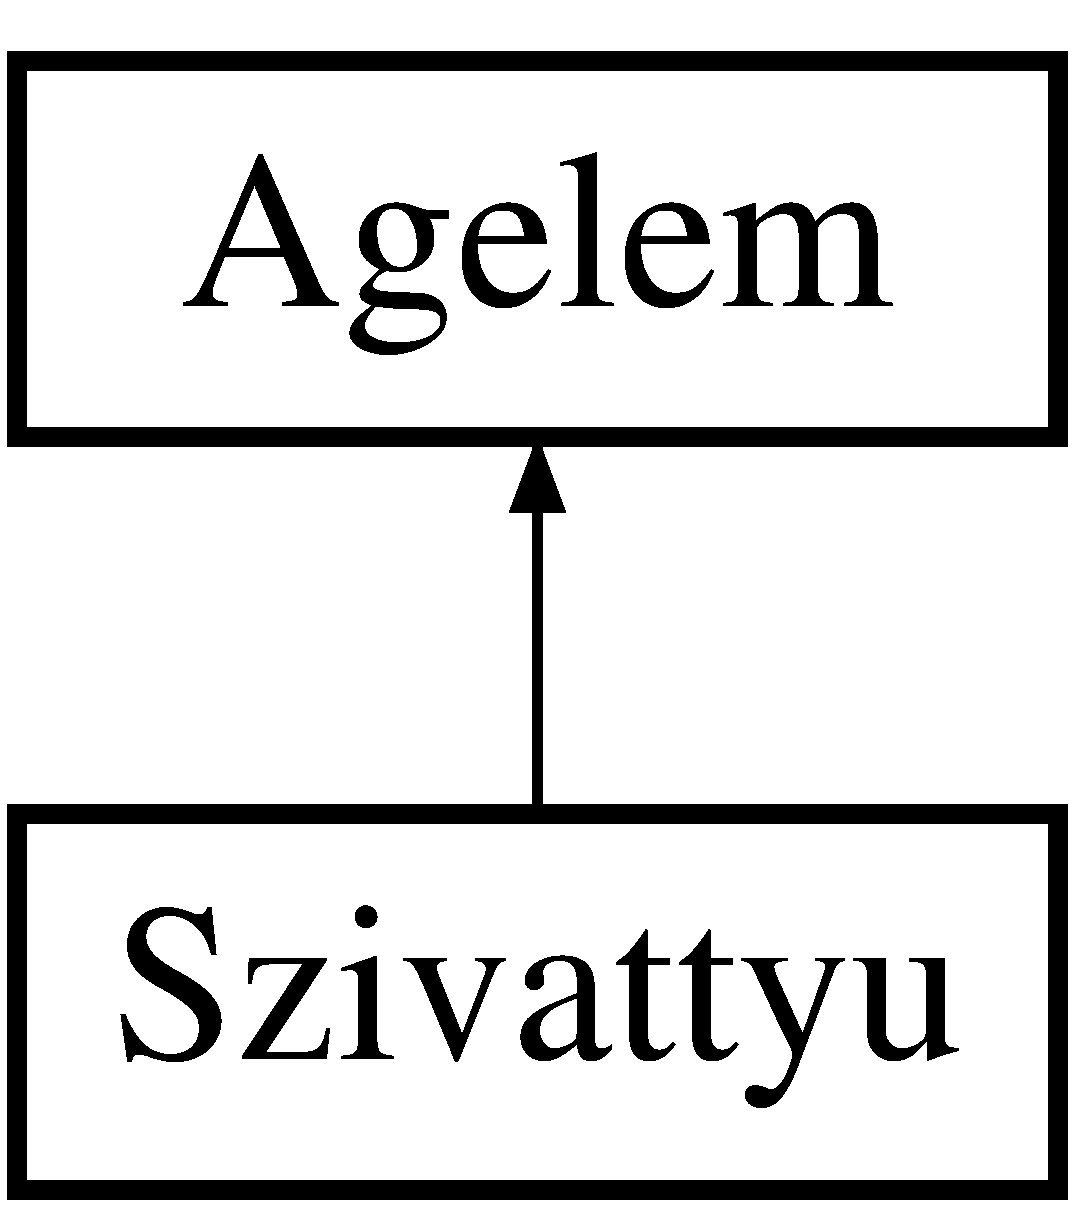
\includegraphics[height=2.000000cm]{class_szivattyu}
\end{center}
\end{figure}
\subsection*{Public Member Functions}
\begin{DoxyCompactItemize}
\item 
{\bfseries Szivattyu} (const string \hyperlink{class_agelem_abe92b7e3912367d5d1caf6b277ca0b7d}{nev}, const string a\+\_\+cspe\+\_\+nev, const string a\+\_\+cspv\+\_\+nev, const double a\+\_\+ro, const double \hyperlink{class_agelem_a3f8668febc2958fd539997d537552f17}{Aref}, const vector$<$ double $>$ q, const vector$<$ double $>$ H, const double a\+\_\+mp)\hypertarget{class_szivattyu_aea7d1a77b34e471145a856483915369f}{}\label{class_szivattyu_aea7d1a77b34e471145a856483915369f}

\item 
string \hyperlink{class_szivattyu_a369c5e45b9381265feeba29d06bd1e59}{Info} ()\hypertarget{class_szivattyu_a369c5e45b9381265feeba29d06bd1e59}{}\label{class_szivattyu_a369c5e45b9381265feeba29d06bd1e59}

\begin{DoxyCompactList}\small\item\em Informacio. \end{DoxyCompactList}\item 
double \hyperlink{class_szivattyu_a083379e0cee2db17f1b20db3fdfcde79}{f} (vector$<$ double $>$)
\begin{DoxyCompactList}\small\item\em Pump branch equation. \end{DoxyCompactList}\item 
vector$<$ double $>$ \hyperlink{class_szivattyu_aefd62e0f02d12273d34511e4b8721f04}{df} (vector$<$ double $>$)\hypertarget{class_szivattyu_aefd62e0f02d12273d34511e4b8721f04}{}\label{class_szivattyu_aefd62e0f02d12273d34511e4b8721f04}

\begin{DoxyCompactList}\small\item\em Jacobi\+: df/dhe, df/dhv, df/dmp, konstans tag. \end{DoxyCompactList}\item 
void \hyperlink{class_szivattyu_a3c35ef43a38a45e9d077281a8804abe4}{Ini} (int mode, double value)\hypertarget{class_szivattyu_a3c35ef43a38a45e9d077281a8804abe4}{}\label{class_szivattyu_a3c35ef43a38a45e9d077281a8804abe4}

\begin{DoxyCompactList}\small\item\em Inicializacio, mode=0 -\/$>$ automatikus, mode=1 -\/$>$ value beirasa. \end{DoxyCompactList}\item 
void {\bfseries Set\+\_\+dprop} (string mit, double mire)\hypertarget{class_szivattyu_aae9b66e4fc0313360d1b8a65ba0a2a68}{}\label{class_szivattyu_aae9b66e4fc0313360d1b8a65ba0a2a68}

\item 
string {\bfseries Get\+Type} ()\hypertarget{class_szivattyu_a373372511e4b9ad88474594052c69a6a}{}\label{class_szivattyu_a373372511e4b9ad88474594052c69a6a}

\item 
double \hyperlink{class_szivattyu_ad2fec54e4e5cb236bc7b6a3e8dfbed2f}{Pump\+Char\+Curve} (double q)
\begin{DoxyCompactList}\small\item\em Pump performance curve evaluation. \end{DoxyCompactList}\item 
double {\bfseries Get\+\_\+\+Pump\+Head\+At} (double q)\hypertarget{class_szivattyu_ad2ddc46a360f9a4de20cae65dd381240}{}\label{class_szivattyu_ad2ddc46a360f9a4de20cae65dd381240}

\end{DoxyCompactItemize}
\subsection*{Additional Inherited Members}


\subsection{Member Function Documentation}
\index{Szivattyu@{Szivattyu}!f@{f}}
\index{f@{f}!Szivattyu@{Szivattyu}}
\subsubsection[{\texorpdfstring{f(vector$<$ double $>$)}{f(vector< double >)}}]{\setlength{\rightskip}{0pt plus 5cm}double Szivattyu\+::f (
\begin{DoxyParamCaption}
\item[{vector$<$ double $>$}]{x}
\end{DoxyParamCaption}
)\hspace{0.3cm}{\ttfamily [virtual]}}\hypertarget{class_szivattyu_a083379e0cee2db17f1b20db3fdfcde79}{}\label{class_szivattyu_a083379e0cee2db17f1b20db3fdfcde79}


Pump branch equation. 

The function evaluates the curve fit by the constructor \begin{DoxySeeAlso}{See also}
\hyperlink{class_szivattyu}{Szivattyu()} 
\end{DoxySeeAlso}

\begin{DoxyParams}{Parameters}
{\em x} & vector$<$double$>$ \\
\hline
{\em x(0)=pstart/ro/g} & \\
\hline
{\em x(1)=pend/ro/g} & \\
\hline
{\em x(2)=zstart} & \\
\hline
{\em x(3)=zend} & \\
\hline
\end{DoxyParams}
\begin{DoxyReturn}{Returns}
(double) function error (should be zero) 
\end{DoxyReturn}
\begin{DoxySeeAlso}{See also}
\hyperlink{class_szivattyu_ad2fec54e4e5cb236bc7b6a3e8dfbed2f}{Pump\+Char\+Curve()} 
\end{DoxySeeAlso}


Implements \hyperlink{class_agelem_aa1d93be52ddae11df003c4e35c47084b}{Agelem}.

\index{Szivattyu@{Szivattyu}!Pump\+Char\+Curve@{Pump\+Char\+Curve}}
\index{Pump\+Char\+Curve@{Pump\+Char\+Curve}!Szivattyu@{Szivattyu}}
\subsubsection[{\texorpdfstring{Pump\+Char\+Curve(double q)}{PumpCharCurve(double q)}}]{\setlength{\rightskip}{0pt plus 5cm}double Szivattyu\+::\+Pump\+Char\+Curve (
\begin{DoxyParamCaption}
\item[{double}]{qq}
\end{DoxyParamCaption}
)}\hypertarget{class_szivattyu_ad2fec54e4e5cb236bc7b6a3e8dfbed2f}{}\label{class_szivattyu_ad2fec54e4e5cb236bc7b6a3e8dfbed2f}


Pump performance curve evaluation. 

The function evaluates the curve fit by the constructor \begin{DoxySeeAlso}{See also}
\hyperlink{class_szivattyu}{Szivattyu()} 
\end{DoxySeeAlso}

\begin{DoxyParams}{Parameters}
{\em qq} & (double) flow rate in m$^\wedge$3/s \\
\hline
\end{DoxyParams}
\begin{DoxyReturn}{Returns}
(double) head in m 
\end{DoxyReturn}
\begin{DoxySeeAlso}{See also}
\hyperlink{class_szivattyu}{Szivattyu()} and \hyperlink{class_szivattyu_a083379e0cee2db17f1b20db3fdfcde79}{f()} 
\end{DoxySeeAlso}


The documentation for this class was generated from the following files\+:\begin{DoxyCompactItemize}
\item 
Szivattyu.\+h\item 
Szivattyu.\+cpp\end{DoxyCompactItemize}

\hypertarget{class_vegakna}{}\section{Vegakna Class Reference}
\label{class_vegakna}\index{Vegakna@{Vegakna}}
Inheritance diagram for Vegakna\+:\begin{figure}[H]
\begin{center}
\leavevmode
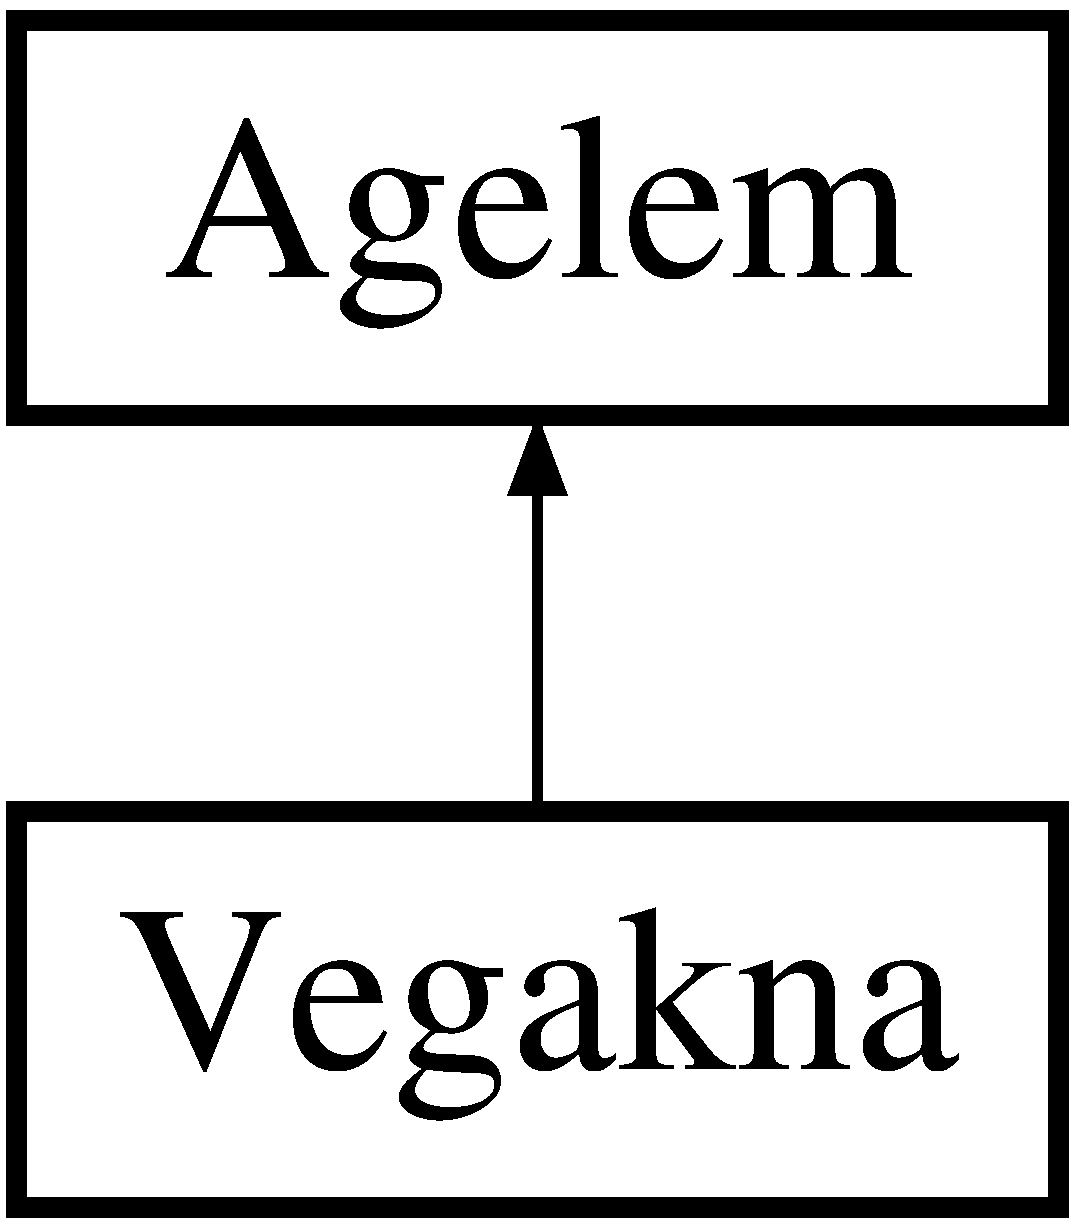
\includegraphics[height=2.000000cm]{class_vegakna}
\end{center}
\end{figure}
\subsection*{Public Member Functions}
\begin{DoxyCompactItemize}
\item 
{\bfseries Vegakna} (const string \hyperlink{class_agelem_abe92b7e3912367d5d1caf6b277ca0b7d}{nev}, const string cspnev, const double a\+\_\+ro, const double \hyperlink{class_agelem_a3f8668febc2958fd539997d537552f17}{Aref}, const double Hf, const double H, const double a\+\_\+mp, const double a\+\_\+tt)\hypertarget{class_vegakna_ae4041ee2a843f526bebded5f99ff2824}{}\label{class_vegakna_ae4041ee2a843f526bebded5f99ff2824}

\item 
string \hyperlink{class_vegakna_a9b47670176b3cff6d577e7a5b7ef7eb2}{Info} ()\hypertarget{class_vegakna_a9b47670176b3cff6d577e7a5b7ef7eb2}{}\label{class_vegakna_a9b47670176b3cff6d577e7a5b7ef7eb2}

\begin{DoxyCompactList}\small\item\em Informacio. \end{DoxyCompactList}\item 
double \hyperlink{class_vegakna_a1f4c98796c6ceb9fbdd935b20af6ab42}{f} (vector$<$ double $>$)\hypertarget{class_vegakna_a1f4c98796c6ceb9fbdd935b20af6ab42}{}\label{class_vegakna_a1f4c98796c6ceb9fbdd935b20af6ab42}

\begin{DoxyCompactList}\small\item\em Az agegyenlet erteke, nullara rendezve, v.\+o.\+m.-\/ben. \end{DoxyCompactList}\item 
vector$<$ double $>$ \hyperlink{class_vegakna_ac76d7d751b9dd9f28b5470ea68625345}{df} (vector$<$ double $>$)\hypertarget{class_vegakna_ac76d7d751b9dd9f28b5470ea68625345}{}\label{class_vegakna_ac76d7d751b9dd9f28b5470ea68625345}

\begin{DoxyCompactList}\small\item\em Jacobi\+: df/dhe, df/dhv, df/dmp, konstans tag. \end{DoxyCompactList}\item 
void \hyperlink{class_vegakna_adaa3748adf56c35c7fb91d014eccb8fe}{Ini} (int mode, double value)\hypertarget{class_vegakna_adaa3748adf56c35c7fb91d014eccb8fe}{}\label{class_vegakna_adaa3748adf56c35c7fb91d014eccb8fe}

\begin{DoxyCompactList}\small\item\em Inicializacio, mode=0 -\/$>$ automatikus, mode=1 -\/$>$ value beirasa. \end{DoxyCompactList}\item 
void {\bfseries Set\+\_\+dprop} (string mit, double mire)\hypertarget{class_vegakna_a6a5d3d90d5e0be90481bdd144c652208}{}\label{class_vegakna_a6a5d3d90d5e0be90481bdd144c652208}

\item 
string {\bfseries Get\+Type} ()\hypertarget{class_vegakna_a623a4d644d9b76f48358738df22b9865}{}\label{class_vegakna_a623a4d644d9b76f48358738df22b9865}

\item 
double \hyperlink{class_vegakna_a262a9880ff91b0d2f0cf3c6f28641913}{Get\+\_\+dprop} (string mit)\hypertarget{class_vegakna_a262a9880ff91b0d2f0cf3c6f28641913}{}\label{class_vegakna_a262a9880ff91b0d2f0cf3c6f28641913}

\begin{DoxyCompactList}\small\item\em Get double property, \hyperlink{class_cso}{Cso} es \hyperlink{class_csatorna}{Csatorna} akarja elulirja. \end{DoxyCompactList}\end{DoxyCompactItemize}
\subsection*{Additional Inherited Members}


The documentation for this class was generated from the following files\+:\begin{DoxyCompactItemize}
\item 
Vegakna.\+h\item 
Vegakna.\+cpp\end{DoxyCompactItemize}

\hypertarget{class_visszacsapo_szelep}{}\section{Visszacsapo\+Szelep Class Reference}
\label{class_visszacsapo_szelep}\index{Visszacsapo\+Szelep@{Visszacsapo\+Szelep}}
Inheritance diagram for Visszacsapo\+Szelep\+:\begin{figure}[H]
\begin{center}
\leavevmode
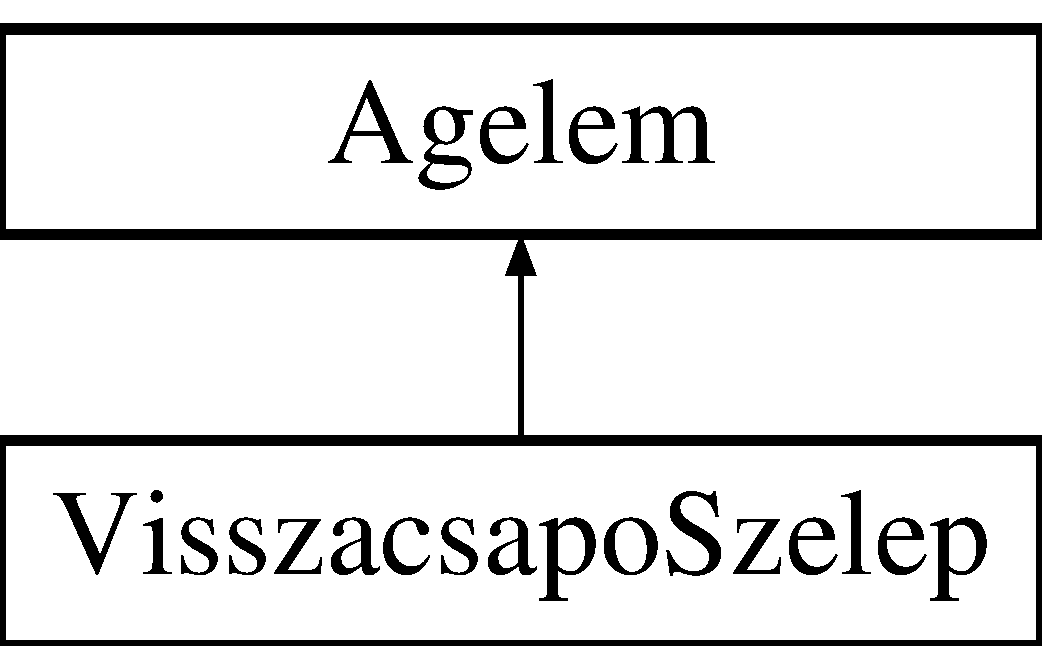
\includegraphics[height=2.000000cm]{class_visszacsapo_szelep}
\end{center}
\end{figure}
\subsection*{Public Member Functions}
\begin{DoxyCompactItemize}
\item 
\hypertarget{class_visszacsapo_szelep_a40da5edbf8243f70eedb5891a0cd6b19}{}\label{class_visszacsapo_szelep_a40da5edbf8243f70eedb5891a0cd6b19} 
{\bfseries Visszacsapo\+Szelep} (const string \hyperlink{class_agelem_abe92b7e3912367d5d1caf6b277ca0b7d}{nev}, const string cspenev, const string cspvnev, const double a\+\_\+ro, const double \hyperlink{class_agelem_a3f8668febc2958fd539997d537552f17}{Aref}, const double veszt\+\_\+e, const double veszt\+\_\+v, const double a\+\_\+mp)
\item 
\hypertarget{class_visszacsapo_szelep_ae4304110869247cb1d1428c366553665}{}\label{class_visszacsapo_szelep_ae4304110869247cb1d1428c366553665} 
string \hyperlink{class_visszacsapo_szelep_ae4304110869247cb1d1428c366553665}{Info} ()
\begin{DoxyCompactList}\small\item\em Informacio. \end{DoxyCompactList}\item 
\hypertarget{class_visszacsapo_szelep_aa148976fb3ca2ab3d35c255dcc83c947}{}\label{class_visszacsapo_szelep_aa148976fb3ca2ab3d35c255dcc83c947} 
double \hyperlink{class_visszacsapo_szelep_aa148976fb3ca2ab3d35c255dcc83c947}{f} (vector$<$ double $>$)
\begin{DoxyCompactList}\small\item\em Az agegyenlet erteke, nullara rendezve, v.\+o.\+m.-\/ben. \end{DoxyCompactList}\item 
\hypertarget{class_visszacsapo_szelep_a9925c2e8f958d4d5707dd563f9d3ff31}{}\label{class_visszacsapo_szelep_a9925c2e8f958d4d5707dd563f9d3ff31} 
vector$<$ double $>$ \hyperlink{class_visszacsapo_szelep_a9925c2e8f958d4d5707dd563f9d3ff31}{df} (vector$<$ double $>$)
\begin{DoxyCompactList}\small\item\em Jacobi\+: df/dhe, df/dhv, df/dmp, konstans tag. \end{DoxyCompactList}\item 
\hypertarget{class_visszacsapo_szelep_a3473fbea667f172b09beae228c730e4f}{}\label{class_visszacsapo_szelep_a3473fbea667f172b09beae228c730e4f} 
void \hyperlink{class_visszacsapo_szelep_a3473fbea667f172b09beae228c730e4f}{Ini} (int mode, double value)
\begin{DoxyCompactList}\small\item\em Inicializacio, mode=0 -\/$>$ automatikus, mode=1 -\/$>$ value beirasa. \end{DoxyCompactList}\item 
\hypertarget{class_visszacsapo_szelep_a926e1eca26c657b4a7c2a6ac90c78729}{}\label{class_visszacsapo_szelep_a926e1eca26c657b4a7c2a6ac90c78729} 
void {\bfseries Set\+\_\+dprop} (string mit, double mire)
\item 
\hypertarget{class_visszacsapo_szelep_aa30043b601103db38fec768e510c3ebe}{}\label{class_visszacsapo_szelep_aa30043b601103db38fec768e510c3ebe} 
string {\bfseries Get\+Type} ()
\end{DoxyCompactItemize}
\subsection*{Additional Inherited Members}


The documentation for this class was generated from the following files\+:\begin{DoxyCompactItemize}
\item 
Visszacsapo\+Szelep.\+h\item 
Visszacsapo\+Szelep.\+cpp\end{DoxyCompactItemize}

\hypertarget{classwavefilt}{}\section{wavefilt Class Reference}
\label{classwavefilt}\index{wavefilt@{wavefilt}}
\subsection*{Public Member Functions}
\begin{DoxyCompactItemize}
\item 
\mbox{\Hypertarget{classwavefilt_a78ae553b7c2cc91677a0750379238492}\label{classwavefilt_a78ae553b7c2cc91677a0750379238492}} 
{\bfseries wavefilt} (const DP $\ast$a, const int n)
\end{DoxyCompactItemize}
\subsection*{Public Attributes}
\begin{DoxyCompactItemize}
\item 
\mbox{\Hypertarget{classwavefilt_acac2c6827e2e4264137cf86c2e6b1889}\label{classwavefilt_acac2c6827e2e4264137cf86c2e6b1889}} 
int {\bfseries ncof}
\item 
\mbox{\Hypertarget{classwavefilt_a99c458cf1dd1dee16139853c85877657}\label{classwavefilt_a99c458cf1dd1dee16139853c85877657}} 
int {\bfseries ioff}
\item 
\mbox{\Hypertarget{classwavefilt_a8758b909c178b3b77576120e6d872f6f}\label{classwavefilt_a8758b909c178b3b77576120e6d872f6f}} 
int {\bfseries joff}
\item 
\mbox{\Hypertarget{classwavefilt_acfccd3c09f69e82dc5272538ff96f4af}\label{classwavefilt_acfccd3c09f69e82dc5272538ff96f4af}} 
\hyperlink{class_n_r_vec}{N\+R\+Vec}$<$ DP $>$ \& {\bfseries cc}
\item 
\mbox{\Hypertarget{classwavefilt_aaef0d62c9f79c72e0f807fbd69654b64}\label{classwavefilt_aaef0d62c9f79c72e0f807fbd69654b64}} 
\hyperlink{class_n_r_vec}{N\+R\+Vec}$<$ DP $>$ \& {\bfseries cr}
\end{DoxyCompactItemize}


The documentation for this class was generated from the following file\+:\begin{DoxyCompactItemize}
\item 
nrutil\+\_\+nr.\+h\end{DoxyCompactItemize}

\hypertarget{struct_x_m_l}{}\section{X\+ML Struct Reference}
\label{struct_x_m_l}\index{X\+ML@{X\+ML}}
\subsection*{Public Attributes}
\begin{DoxyCompactItemize}
\item 
\hypertarget{struct_x_m_l_a85d57b749883255ab1c4533919d3d271}{}\label{struct_x_m_l_a85d57b749883255ab1c4533919d3d271} 
X\+M\+L\+C\+S\+TR {\bfseries lp\+X\+ML}
\item 
\hypertarget{struct_x_m_l_a8b9e70c05d1307204056dfb882d6dcff}{}\label{struct_x_m_l_a8b9e70c05d1307204056dfb882d6dcff} 
X\+M\+L\+C\+S\+TR {\bfseries lpsz\+Text}
\item 
\hypertarget{struct_x_m_l_a73a28b836fcc0656097c7e751b87460d}{}\label{struct_x_m_l_a73a28b836fcc0656097c7e751b87460d} 
int {\bfseries n\+Index}
\item 
\hypertarget{struct_x_m_l_a31832d9cbe0dc08449dbededa9a2d469}{}\label{struct_x_m_l_a31832d9cbe0dc08449dbededa9a2d469} 
int {\bfseries n\+Index\+Missig\+End\+Tag}
\item 
\hypertarget{struct_x_m_l_a843061b60ba6ab66bf855741142facd2}{}\label{struct_x_m_l_a843061b60ba6ab66bf855741142facd2} 
enum X\+M\+L\+Error {\bfseries error}
\item 
\hypertarget{struct_x_m_l_a7d04adf93bf8ad8f07b702bc171a9cdb}{}\label{struct_x_m_l_a7d04adf93bf8ad8f07b702bc171a9cdb} 
X\+M\+L\+C\+S\+TR {\bfseries lp\+End\+Tag}
\item 
\hypertarget{struct_x_m_l_a73e0e13cd36312460aa828627b75a285}{}\label{struct_x_m_l_a73e0e13cd36312460aa828627b75a285} 
int {\bfseries cb\+End\+Tag}
\item 
\hypertarget{struct_x_m_l_a1dea7c007c6cbbf7097e1f8d726cef0e}{}\label{struct_x_m_l_a1dea7c007c6cbbf7097e1f8d726cef0e} 
X\+M\+L\+C\+S\+TR {\bfseries lp\+New\+Element}
\item 
\hypertarget{struct_x_m_l_a704f366b471b30e618951c1335e8b01c}{}\label{struct_x_m_l_a704f366b471b30e618951c1335e8b01c} 
int {\bfseries cb\+New\+Element}
\item 
\hypertarget{struct_x_m_l_a49f39e41382ff416ec5c0b5aedfd3735}{}\label{struct_x_m_l_a49f39e41382ff416ec5c0b5aedfd3735} 
int {\bfseries n\+First}
\end{DoxyCompactItemize}


The documentation for this struct was generated from the following file\+:\begin{DoxyCompactItemize}
\item 
xml\+Parser.\+cpp\end{DoxyCompactItemize}

\hypertarget{struct_x_m_l_attribute}{}\section{X\+M\+L\+Attribute Struct Reference}
\label{struct_x_m_l_attribute}\index{X\+M\+L\+Attribute@{X\+M\+L\+Attribute}}
\subsection*{Public Attributes}
\begin{DoxyCompactItemize}
\item 
\mbox{\Hypertarget{struct_x_m_l_attribute_a59d24e06998261f56a5b8e2f2b20ea9e}\label{struct_x_m_l_attribute_a59d24e06998261f56a5b8e2f2b20ea9e}} 
X\+M\+L\+C\+S\+TR {\bfseries lpsz\+Name}
\item 
\mbox{\Hypertarget{struct_x_m_l_attribute_a2e1317aefc63d17247e3e12091b90618}\label{struct_x_m_l_attribute_a2e1317aefc63d17247e3e12091b90618}} 
X\+M\+L\+C\+S\+TR {\bfseries lpsz\+Value}
\end{DoxyCompactItemize}


The documentation for this struct was generated from the following file\+:\begin{DoxyCompactItemize}
\item 
xml\+Parser.\+h\end{DoxyCompactItemize}

\hypertarget{struct_x_m_l_character_entity}{}\section{X\+M\+L\+Character\+Entity Struct Reference}
\label{struct_x_m_l_character_entity}\index{X\+M\+L\+Character\+Entity@{X\+M\+L\+Character\+Entity}}
\subsection*{Public Attributes}
\begin{DoxyCompactItemize}
\item 
\mbox{\Hypertarget{struct_x_m_l_character_entity_ab40240376cadfe2b03a63e83c5947e75}\label{struct_x_m_l_character_entity_ab40240376cadfe2b03a63e83c5947e75}} 
X\+M\+L\+C\+S\+TR {\bfseries s}
\item 
\mbox{\Hypertarget{struct_x_m_l_character_entity_aff111c73a82954b0ae63b75cc6c66214}\label{struct_x_m_l_character_entity_aff111c73a82954b0ae63b75cc6c66214}} 
int {\bfseries l}
\item 
\mbox{\Hypertarget{struct_x_m_l_character_entity_a8c5ed14bcc92397808660ac05509f714}\label{struct_x_m_l_character_entity_a8c5ed14bcc92397808660ac05509f714}} 
X\+M\+L\+C\+H\+AR {\bfseries c}
\end{DoxyCompactItemize}


The documentation for this struct was generated from the following file\+:\begin{DoxyCompactItemize}
\item 
xml\+Parser.\+cpp\end{DoxyCompactItemize}

\hypertarget{struct_x_m_l_clear}{}\section{X\+M\+L\+Clear Struct Reference}
\label{struct_x_m_l_clear}\index{X\+M\+L\+Clear@{X\+M\+L\+Clear}}
\subsection*{Public Attributes}
\begin{DoxyCompactItemize}
\item 
X\+M\+L\+C\+S\+TR {\bfseries lpsz\+Value}\hypertarget{struct_x_m_l_clear_a72d26ba6f77bdfc5fdaf0e0802d8809e}{}\label{struct_x_m_l_clear_a72d26ba6f77bdfc5fdaf0e0802d8809e}

\item 
X\+M\+L\+C\+S\+TR {\bfseries lpsz\+Open\+Tag}\hypertarget{struct_x_m_l_clear_a2df4ad4786cc0d3f7eae94607a02f6e3}{}\label{struct_x_m_l_clear_a2df4ad4786cc0d3f7eae94607a02f6e3}

\item 
X\+M\+L\+C\+S\+TR {\bfseries lpsz\+Close\+Tag}\hypertarget{struct_x_m_l_clear_a28c30d46f2965cfdea9dcd7ff10e0386}{}\label{struct_x_m_l_clear_a28c30d46f2965cfdea9dcd7ff10e0386}

\end{DoxyCompactItemize}


The documentation for this struct was generated from the following file\+:\begin{DoxyCompactItemize}
\item 
xml\+Parser.\+h\end{DoxyCompactItemize}

\hypertarget{struct_x_m_l_node}{}\section{X\+M\+L\+Node Struct Reference}
\label{struct_x_m_l_node}\index{X\+M\+L\+Node@{X\+M\+L\+Node}}
\subsection*{Public Member Functions}
\begin{DoxyCompactItemize}
\item 
\hypertarget{struct_x_m_l_node_a78f873d053775e62bbe7e9b9ba9a0893}{}\label{struct_x_m_l_node_a78f873d053775e62bbe7e9b9ba9a0893} 
X\+M\+L\+C\+S\+TR {\bfseries get\+Name} () const
\item 
\hypertarget{struct_x_m_l_node_acfe86b318bec6ed981ec2ede1b82a01c}{}\label{struct_x_m_l_node_acfe86b318bec6ed981ec2ede1b82a01c} 
X\+M\+L\+C\+S\+TR {\bfseries get\+Text} (int i=0) const
\item 
\hypertarget{struct_x_m_l_node_a1cab1484d301f5b99a5fc74a0b05b47e}{}\label{struct_x_m_l_node_a1cab1484d301f5b99a5fc74a0b05b47e} 
int {\bfseries n\+Text} () const
\item 
\hypertarget{struct_x_m_l_node_a4c1de07d0e519c6e1d54d855b47d9d6a}{}\label{struct_x_m_l_node_a4c1de07d0e519c6e1d54d855b47d9d6a} 
\hyperlink{struct_x_m_l_node}{X\+M\+L\+Node} {\bfseries get\+Parent\+Node} () const
\item 
\hypertarget{struct_x_m_l_node_ac34f1bdbf808d2ee89552415505bb673}{}\label{struct_x_m_l_node_ac34f1bdbf808d2ee89552415505bb673} 
\hyperlink{struct_x_m_l_node}{X\+M\+L\+Node} {\bfseries get\+Child\+Node} (int i=0) const
\item 
\hypertarget{struct_x_m_l_node_af082d930c7bc6f879ab282adbe48050f}{}\label{struct_x_m_l_node_af082d930c7bc6f879ab282adbe48050f} 
\hyperlink{struct_x_m_l_node}{X\+M\+L\+Node} {\bfseries get\+Child\+Node} (X\+M\+L\+C\+S\+TR name, int i) const
\item 
\hypertarget{struct_x_m_l_node_ae67a570d76c61d12d26a309f4c5645e2}{}\label{struct_x_m_l_node_ae67a570d76c61d12d26a309f4c5645e2} 
\hyperlink{struct_x_m_l_node}{X\+M\+L\+Node} {\bfseries get\+Child\+Node} (X\+M\+L\+C\+S\+TR name, int $\ast$i=N\+U\+LL) const
\item 
\hypertarget{struct_x_m_l_node_ad2665e479c488e525eba26659fe4034d}{}\label{struct_x_m_l_node_ad2665e479c488e525eba26659fe4034d} 
\hyperlink{struct_x_m_l_node}{X\+M\+L\+Node} {\bfseries get\+Child\+Node\+With\+Attribute} (X\+M\+L\+C\+S\+TR tag\+Name, X\+M\+L\+C\+S\+TR attribute\+Name, X\+M\+L\+C\+S\+TR attribute\+Value=N\+U\+LL, int $\ast$i=N\+U\+LL) const
\item 
\hypertarget{struct_x_m_l_node_a37dfb85db6b3e8974474c9a6277fff94}{}\label{struct_x_m_l_node_a37dfb85db6b3e8974474c9a6277fff94} 
int {\bfseries n\+Child\+Node} (X\+M\+L\+C\+S\+TR name) const
\item 
\hypertarget{struct_x_m_l_node_a89884092225798f347305956c1ecc62b}{}\label{struct_x_m_l_node_a89884092225798f347305956c1ecc62b} 
int {\bfseries n\+Child\+Node} () const
\item 
\hypertarget{struct_x_m_l_node_a50cc434e59c5f24f70eec2ae4b0554ab}{}\label{struct_x_m_l_node_a50cc434e59c5f24f70eec2ae4b0554ab} 
\hyperlink{struct_x_m_l_attribute}{X\+M\+L\+Attribute} {\bfseries get\+Attribute} (int i=0) const
\item 
\hypertarget{struct_x_m_l_node_a6710fba2ad2ca7c79c3e5d17a2101e08}{}\label{struct_x_m_l_node_a6710fba2ad2ca7c79c3e5d17a2101e08} 
X\+M\+L\+C\+S\+TR {\bfseries get\+Attribute\+Name} (int i=0) const
\item 
\hypertarget{struct_x_m_l_node_a48375d3bbdff5a0f416f668498edd3cb}{}\label{struct_x_m_l_node_a48375d3bbdff5a0f416f668498edd3cb} 
X\+M\+L\+C\+S\+TR {\bfseries get\+Attribute\+Value} (int i=0) const
\item 
\hypertarget{struct_x_m_l_node_a0bf031a1bca5c211810eb3420595589e}{}\label{struct_x_m_l_node_a0bf031a1bca5c211810eb3420595589e} 
char {\bfseries is\+Attribute\+Set} (X\+M\+L\+C\+S\+TR name) const
\item 
\hypertarget{struct_x_m_l_node_a5b66e8469c1f6c3398993e38981ead13}{}\label{struct_x_m_l_node_a5b66e8469c1f6c3398993e38981ead13} 
X\+M\+L\+C\+S\+TR {\bfseries get\+Attribute} (X\+M\+L\+C\+S\+TR name, int i) const
\item 
\hypertarget{struct_x_m_l_node_aed21862233be12773795cf6f3b9feeed}{}\label{struct_x_m_l_node_aed21862233be12773795cf6f3b9feeed} 
X\+M\+L\+C\+S\+TR {\bfseries get\+Attribute} (X\+M\+L\+C\+S\+TR name, int $\ast$i=N\+U\+LL) const
\item 
\hypertarget{struct_x_m_l_node_a7980a71afeab26b29c4f1c67659d4214}{}\label{struct_x_m_l_node_a7980a71afeab26b29c4f1c67659d4214} 
int {\bfseries n\+Attribute} () const
\item 
\hypertarget{struct_x_m_l_node_ae1fcdd6a5e7c33b8c3c42ceb695a8a92}{}\label{struct_x_m_l_node_ae1fcdd6a5e7c33b8c3c42ceb695a8a92} 
\hyperlink{struct_x_m_l_clear}{X\+M\+L\+Clear} {\bfseries get\+Clear} (int i=0) const
\item 
\hypertarget{struct_x_m_l_node_ac698d5a2e8e8eac2d212d84013c4b0e8}{}\label{struct_x_m_l_node_ac698d5a2e8e8eac2d212d84013c4b0e8} 
int {\bfseries n\+Clear} () const
\item 
\hypertarget{struct_x_m_l_node_a9e19d3587f88f503ff1cfd98fcd13cb1}{}\label{struct_x_m_l_node_a9e19d3587f88f503ff1cfd98fcd13cb1} 
X\+M\+L\+S\+TR {\bfseries create\+X\+M\+L\+String} (int n\+Format=1, int $\ast$pn\+Size=N\+U\+LL) const
\item 
\hypertarget{struct_x_m_l_node_acef9de855bd31c6cda5482cb296f28ae}{}\label{struct_x_m_l_node_acef9de855bd31c6cda5482cb296f28ae} 
X\+M\+L\+Error {\bfseries write\+To\+File} (X\+M\+L\+C\+S\+TR filename, const char $\ast$encoding=N\+U\+LL, char n\+Format=1) const
\item 
\hypertarget{struct_x_m_l_node_a2406beecada2b815907eaac2c7db035b}{}\label{struct_x_m_l_node_a2406beecada2b815907eaac2c7db035b} 
\hyperlink{struct_x_m_l_node_contents}{X\+M\+L\+Node\+Contents} {\bfseries enum\+Contents} (int i) const
\item 
\hypertarget{struct_x_m_l_node_a1b13a6dc1cb8e7248caedd4960d7ba60}{}\label{struct_x_m_l_node_a1b13a6dc1cb8e7248caedd4960d7ba60} 
int {\bfseries n\+Element} () const
\item 
\hypertarget{struct_x_m_l_node_ab888c4755daee4a2f976713531f1e3c3}{}\label{struct_x_m_l_node_ab888c4755daee4a2f976713531f1e3c3} 
char {\bfseries is\+Empty} () const
\item 
\hypertarget{struct_x_m_l_node_affcffca699c492a1d26a037e958c14f5}{}\label{struct_x_m_l_node_affcffca699c492a1d26a037e958c14f5} 
char {\bfseries is\+Declaration} () const
\item 
\hypertarget{struct_x_m_l_node_a138099a1355b9d4103c239d9042adad3}{}\label{struct_x_m_l_node_a138099a1355b9d4103c239d9042adad3} 
{\bfseries X\+M\+L\+Node} (const \hyperlink{struct_x_m_l_node}{X\+M\+L\+Node} \&A)
\item 
\hypertarget{struct_x_m_l_node_ac7201d06ce47509423dd7cc937e69cf8}{}\label{struct_x_m_l_node_ac7201d06ce47509423dd7cc937e69cf8} 
\hyperlink{struct_x_m_l_node}{X\+M\+L\+Node} \& {\bfseries operator=} (const \hyperlink{struct_x_m_l_node}{X\+M\+L\+Node} \&A)
\item 
\hypertarget{struct_x_m_l_node_a71645ec6bcd94ff4bff62810377954ce}{}\label{struct_x_m_l_node_a71645ec6bcd94ff4bff62810377954ce} 
\hyperlink{struct_x_m_l_node}{X\+M\+L\+Node} {\bfseries add\+Child} (X\+M\+L\+C\+S\+TR lpsz\+Name, char is\+Declaration=F\+A\+L\+SE, int pos=-\/1)
\item 
\hypertarget{struct_x_m_l_node_a7938c43648ce7ed32efc9f0a5e3b5d2c}{}\label{struct_x_m_l_node_a7938c43648ce7ed32efc9f0a5e3b5d2c} 
\hyperlink{struct_x_m_l_attribute}{X\+M\+L\+Attribute} $\ast$ {\bfseries add\+Attribute} (X\+M\+L\+C\+S\+TR lpsz\+Name, X\+M\+L\+C\+S\+TR lpsz\+Valuev)
\item 
\hypertarget{struct_x_m_l_node_aa4210523be86adbfb39ad52469a9a072}{}\label{struct_x_m_l_node_aa4210523be86adbfb39ad52469a9a072} 
X\+M\+L\+C\+S\+TR {\bfseries add\+Text} (X\+M\+L\+C\+S\+TR lpsz\+Value, int pos=-\/1)
\item 
\hypertarget{struct_x_m_l_node_ad98c759ea686cd8b30314259f942aabf}{}\label{struct_x_m_l_node_ad98c759ea686cd8b30314259f942aabf} 
\hyperlink{struct_x_m_l_clear}{X\+M\+L\+Clear} $\ast$ {\bfseries add\+Clear} (X\+M\+L\+C\+S\+TR lpsz\+Value, X\+M\+L\+C\+S\+TR lpsz\+Open=N\+U\+LL, X\+M\+L\+C\+S\+TR lpsz\+Close=N\+U\+LL, int pos=-\/1)
\item 
\hypertarget{struct_x_m_l_node_adcb76cce8d914425b03fdd9a06ee2a47}{}\label{struct_x_m_l_node_adcb76cce8d914425b03fdd9a06ee2a47} 
\hyperlink{struct_x_m_l_node}{X\+M\+L\+Node} {\bfseries add\+Child} (\hyperlink{struct_x_m_l_node}{X\+M\+L\+Node} node\+To\+Add, int pos=-\/1)
\item 
\hypertarget{struct_x_m_l_node_ae08b643a2b87a77bad3c70eb57ea3043}{}\label{struct_x_m_l_node_ae08b643a2b87a77bad3c70eb57ea3043} 
X\+M\+L\+C\+S\+TR {\bfseries update\+Name} (X\+M\+L\+C\+S\+TR lpsz\+Name)
\item 
\hypertarget{struct_x_m_l_node_adfbd017929a40d6584350e7f3652fcbd}{}\label{struct_x_m_l_node_adfbd017929a40d6584350e7f3652fcbd} 
\hyperlink{struct_x_m_l_attribute}{X\+M\+L\+Attribute} $\ast$ {\bfseries update\+Attribute} (\hyperlink{struct_x_m_l_attribute}{X\+M\+L\+Attribute} $\ast$new\+Attribute, \hyperlink{struct_x_m_l_attribute}{X\+M\+L\+Attribute} $\ast$old\+Attribute)
\item 
\hypertarget{struct_x_m_l_node_a21bdabc3bea95c06b5033a0a0c76afe4}{}\label{struct_x_m_l_node_a21bdabc3bea95c06b5033a0a0c76afe4} 
\hyperlink{struct_x_m_l_attribute}{X\+M\+L\+Attribute} $\ast$ {\bfseries update\+Attribute} (X\+M\+L\+C\+S\+TR lpsz\+New\+Value, X\+M\+L\+C\+S\+TR lpsz\+New\+Name=N\+U\+LL, int i=0)
\item 
\hypertarget{struct_x_m_l_node_ab81bdf55327b63350eaf84835b8cf9b1}{}\label{struct_x_m_l_node_ab81bdf55327b63350eaf84835b8cf9b1} 
\hyperlink{struct_x_m_l_attribute}{X\+M\+L\+Attribute} $\ast$ {\bfseries update\+Attribute} (X\+M\+L\+C\+S\+TR lpsz\+New\+Value, X\+M\+L\+C\+S\+TR lpsz\+New\+Name, X\+M\+L\+C\+S\+TR lpsz\+Old\+Name)
\item 
\hypertarget{struct_x_m_l_node_aad04ffd86ca67253bbc81f941608f8d2}{}\label{struct_x_m_l_node_aad04ffd86ca67253bbc81f941608f8d2} 
X\+M\+L\+C\+S\+TR {\bfseries update\+Text} (X\+M\+L\+C\+S\+TR lpsz\+New\+Value, int i=0)
\item 
\hypertarget{struct_x_m_l_node_a476a872fa595ea8416d2991ce3bea7a6}{}\label{struct_x_m_l_node_a476a872fa595ea8416d2991ce3bea7a6} 
X\+M\+L\+C\+S\+TR {\bfseries update\+Text} (X\+M\+L\+C\+S\+TR lpsz\+New\+Value, X\+M\+L\+C\+S\+TR lpsz\+Old\+Value)
\item 
\hypertarget{struct_x_m_l_node_a6b48e123943ea53272f6d4be33ca6d04}{}\label{struct_x_m_l_node_a6b48e123943ea53272f6d4be33ca6d04} 
\hyperlink{struct_x_m_l_clear}{X\+M\+L\+Clear} $\ast$ {\bfseries update\+Clear} (X\+M\+L\+C\+S\+TR lpsz\+New\+Content, int i=0)
\item 
\hypertarget{struct_x_m_l_node_a02e1a7e3f9c48e05fad77abda2116375}{}\label{struct_x_m_l_node_a02e1a7e3f9c48e05fad77abda2116375} 
\hyperlink{struct_x_m_l_clear}{X\+M\+L\+Clear} $\ast$ {\bfseries update\+Clear} (\hyperlink{struct_x_m_l_clear}{X\+M\+L\+Clear} $\ast$newP, \hyperlink{struct_x_m_l_clear}{X\+M\+L\+Clear} $\ast$oldP)
\item 
\hypertarget{struct_x_m_l_node_a690b140b6d86776f3a257a42ce7d4948}{}\label{struct_x_m_l_node_a690b140b6d86776f3a257a42ce7d4948} 
\hyperlink{struct_x_m_l_clear}{X\+M\+L\+Clear} $\ast$ {\bfseries update\+Clear} (X\+M\+L\+C\+S\+TR lpsz\+New\+Value, X\+M\+L\+C\+S\+TR lpsz\+Old\+Value)
\item 
\hypertarget{struct_x_m_l_node_abbb236ca1081f145a04bce9ea03c62a6}{}\label{struct_x_m_l_node_abbb236ca1081f145a04bce9ea03c62a6} 
void {\bfseries delete\+Node\+Content} (char force=0)
\item 
\hypertarget{struct_x_m_l_node_a2b21339e5b370f1d7ebde2dc51217eed}{}\label{struct_x_m_l_node_a2b21339e5b370f1d7ebde2dc51217eed} 
void {\bfseries delete\+Attribute} (X\+M\+L\+C\+S\+TR lpsz\+Name)
\item 
\hypertarget{struct_x_m_l_node_a61b2405305063594b35b309cc2e22c01}{}\label{struct_x_m_l_node_a61b2405305063594b35b309cc2e22c01} 
void {\bfseries delete\+Attribute} (int i=0)
\item 
\hypertarget{struct_x_m_l_node_a6f00d7c1b4eaa29cfdd9d4a709495aca}{}\label{struct_x_m_l_node_a6f00d7c1b4eaa29cfdd9d4a709495aca} 
void {\bfseries delete\+Attribute} (\hyperlink{struct_x_m_l_attribute}{X\+M\+L\+Attribute} $\ast$an\+Attribute)
\item 
\hypertarget{struct_x_m_l_node_a14a49a23735ea10a44864cb6b4302250}{}\label{struct_x_m_l_node_a14a49a23735ea10a44864cb6b4302250} 
void {\bfseries delete\+Text} (int i=0)
\item 
\hypertarget{struct_x_m_l_node_a21ee499630d71ab6026753a85f02f582}{}\label{struct_x_m_l_node_a21ee499630d71ab6026753a85f02f582} 
void {\bfseries delete\+Text} (X\+M\+L\+C\+S\+TR lpsz\+Value)
\item 
\hypertarget{struct_x_m_l_node_a44b72c82310eb4319dba46eb9cc9f6e9}{}\label{struct_x_m_l_node_a44b72c82310eb4319dba46eb9cc9f6e9} 
void {\bfseries delete\+Clear} (int i=0)
\item 
\hypertarget{struct_x_m_l_node_ae92182823d3d5b40893103ad222ec4a8}{}\label{struct_x_m_l_node_ae92182823d3d5b40893103ad222ec4a8} 
void {\bfseries delete\+Clear} (\hyperlink{struct_x_m_l_clear}{X\+M\+L\+Clear} $\ast$p)
\item 
\hypertarget{struct_x_m_l_node_a8fff4baa9a8000f8662ee302438fff64}{}\label{struct_x_m_l_node_a8fff4baa9a8000f8662ee302438fff64} 
void {\bfseries delete\+Clear} (X\+M\+L\+C\+S\+TR lpsz\+Value)
\item 
\hypertarget{struct_x_m_l_node_acb8f9583792c008c80a6c788f3dedf39}{}\label{struct_x_m_l_node_acb8f9583792c008c80a6c788f3dedf39} 
\hyperlink{struct_x_m_l_node}{X\+M\+L\+Node} {\bfseries add\+Child\+\_\+\+W\+O\+SD} (X\+M\+L\+C\+S\+TR lpsz\+Name, char is\+Declaration=F\+A\+L\+SE, int pos=-\/1)
\item 
\hypertarget{struct_x_m_l_node_a776e46bdd596a7eff1d2dd4105c64034}{}\label{struct_x_m_l_node_a776e46bdd596a7eff1d2dd4105c64034} 
\hyperlink{struct_x_m_l_attribute}{X\+M\+L\+Attribute} $\ast$ {\bfseries add\+Attribute\+\_\+\+W\+O\+SD} (X\+M\+L\+C\+S\+TR lpsz\+Name, X\+M\+L\+C\+S\+TR lpsz\+Value)
\item 
\hypertarget{struct_x_m_l_node_ab05f39710a61064adf3af30fd430acf2}{}\label{struct_x_m_l_node_ab05f39710a61064adf3af30fd430acf2} 
X\+M\+L\+C\+S\+TR {\bfseries add\+Text\+\_\+\+W\+O\+SD} (X\+M\+L\+C\+S\+TR lpsz\+Value, int pos=-\/1)
\item 
\hypertarget{struct_x_m_l_node_a6ea1fad6ada2038f5cf2605839694d31}{}\label{struct_x_m_l_node_a6ea1fad6ada2038f5cf2605839694d31} 
\hyperlink{struct_x_m_l_clear}{X\+M\+L\+Clear} $\ast$ {\bfseries add\+Clear\+\_\+\+W\+O\+SD} (X\+M\+L\+C\+S\+TR lpsz\+Value, X\+M\+L\+C\+S\+TR lpsz\+Open=N\+U\+LL, X\+M\+L\+C\+S\+TR lpsz\+Close=N\+U\+LL, int pos=-\/1)
\item 
\hypertarget{struct_x_m_l_node_af7cff0d6f43d4e6f163f2738a71ec4e5}{}\label{struct_x_m_l_node_af7cff0d6f43d4e6f163f2738a71ec4e5} 
X\+M\+L\+C\+S\+TR {\bfseries update\+Name\+\_\+\+W\+O\+SD} (X\+M\+L\+C\+S\+TR lpsz\+Name)
\item 
\hypertarget{struct_x_m_l_node_a62a2c0cad7809a03afc485351c9560da}{}\label{struct_x_m_l_node_a62a2c0cad7809a03afc485351c9560da} 
\hyperlink{struct_x_m_l_attribute}{X\+M\+L\+Attribute} $\ast$ {\bfseries update\+Attribute\+\_\+\+W\+O\+SD} (\hyperlink{struct_x_m_l_attribute}{X\+M\+L\+Attribute} $\ast$new\+Attribute, \hyperlink{struct_x_m_l_attribute}{X\+M\+L\+Attribute} $\ast$old\+Attribute)
\item 
\hypertarget{struct_x_m_l_node_aab4e4f09a253842ec329f3af90b74cf9}{}\label{struct_x_m_l_node_aab4e4f09a253842ec329f3af90b74cf9} 
\hyperlink{struct_x_m_l_attribute}{X\+M\+L\+Attribute} $\ast$ {\bfseries update\+Attribute\+\_\+\+W\+O\+SD} (X\+M\+L\+C\+S\+TR lpsz\+New\+Value, X\+M\+L\+C\+S\+TR lpsz\+New\+Name=N\+U\+LL, int i=0)
\item 
\hypertarget{struct_x_m_l_node_a25e0857638217206b11ee8fe99f7ed86}{}\label{struct_x_m_l_node_a25e0857638217206b11ee8fe99f7ed86} 
\hyperlink{struct_x_m_l_attribute}{X\+M\+L\+Attribute} $\ast$ {\bfseries update\+Attribute\+\_\+\+W\+O\+SD} (X\+M\+L\+C\+S\+TR lpsz\+New\+Value, X\+M\+L\+C\+S\+TR lpsz\+New\+Name, X\+M\+L\+C\+S\+TR lpsz\+Old\+Name)
\item 
\hypertarget{struct_x_m_l_node_adcff1825b8c39743e35df76db9d0a72d}{}\label{struct_x_m_l_node_adcff1825b8c39743e35df76db9d0a72d} 
X\+M\+L\+C\+S\+TR {\bfseries update\+Text\+\_\+\+W\+O\+SD} (X\+M\+L\+C\+S\+TR lpsz\+New\+Value, int i=0)
\item 
\hypertarget{struct_x_m_l_node_a79d26f52b800cb5f413cda3b08c4b89b}{}\label{struct_x_m_l_node_a79d26f52b800cb5f413cda3b08c4b89b} 
X\+M\+L\+C\+S\+TR {\bfseries update\+Text\+\_\+\+W\+O\+SD} (X\+M\+L\+C\+S\+TR lpsz\+New\+Value, X\+M\+L\+C\+S\+TR lpsz\+Old\+Value)
\item 
\hypertarget{struct_x_m_l_node_a70340d5baee0f1789149b459c9861b03}{}\label{struct_x_m_l_node_a70340d5baee0f1789149b459c9861b03} 
\hyperlink{struct_x_m_l_clear}{X\+M\+L\+Clear} $\ast$ {\bfseries update\+Clear\+\_\+\+W\+O\+SD} (X\+M\+L\+C\+S\+TR lpsz\+New\+Content, int i=0)
\item 
\hypertarget{struct_x_m_l_node_a25a713d21457706eabd8658bbce0b180}{}\label{struct_x_m_l_node_a25a713d21457706eabd8658bbce0b180} 
\hyperlink{struct_x_m_l_clear}{X\+M\+L\+Clear} $\ast$ {\bfseries update\+Clear\+\_\+\+W\+O\+SD} (\hyperlink{struct_x_m_l_clear}{X\+M\+L\+Clear} $\ast$newP, \hyperlink{struct_x_m_l_clear}{X\+M\+L\+Clear} $\ast$oldP)
\item 
\hypertarget{struct_x_m_l_node_a0b46f3ed1681e355e30120c43c410767}{}\label{struct_x_m_l_node_a0b46f3ed1681e355e30120c43c410767} 
\hyperlink{struct_x_m_l_clear}{X\+M\+L\+Clear} $\ast$ {\bfseries update\+Clear\+\_\+\+W\+O\+SD} (X\+M\+L\+C\+S\+TR lpsz\+New\+Value, X\+M\+L\+C\+S\+TR lpsz\+Old\+Value)
\item 
\hypertarget{struct_x_m_l_node_a3037f2fb4ce172d3f5156d9707af5c10}{}\label{struct_x_m_l_node_a3037f2fb4ce172d3f5156d9707af5c10} 
int {\bfseries position\+Of\+Text} (int i=0) const
\item 
\hypertarget{struct_x_m_l_node_a23d8731aafccd6153a3a7351a80b278e}{}\label{struct_x_m_l_node_a23d8731aafccd6153a3a7351a80b278e} 
int {\bfseries position\+Of\+Text} (X\+M\+L\+C\+S\+TR lpsz\+Value) const
\item 
\hypertarget{struct_x_m_l_node_a5ac10cf45468302f26d4932bf4678a95}{}\label{struct_x_m_l_node_a5ac10cf45468302f26d4932bf4678a95} 
int {\bfseries position\+Of\+Clear} (int i=0) const
\item 
\hypertarget{struct_x_m_l_node_ab0cab901f9feff22a76929d011e7a08d}{}\label{struct_x_m_l_node_ab0cab901f9feff22a76929d011e7a08d} 
int {\bfseries position\+Of\+Clear} (X\+M\+L\+C\+S\+TR lpsz\+Value) const
\item 
\hypertarget{struct_x_m_l_node_a04d7989f7a460a1bcd200be5376e2467}{}\label{struct_x_m_l_node_a04d7989f7a460a1bcd200be5376e2467} 
int {\bfseries position\+Of\+Clear} (\hyperlink{struct_x_m_l_clear}{X\+M\+L\+Clear} $\ast$a) const
\item 
\hypertarget{struct_x_m_l_node_a325d7fa417ea2461e03792386cbebdef}{}\label{struct_x_m_l_node_a325d7fa417ea2461e03792386cbebdef} 
int {\bfseries position\+Of\+Child\+Node} (int i=0) const
\item 
\hypertarget{struct_x_m_l_node_a1e28b439f9616c680fd0af893de67c01}{}\label{struct_x_m_l_node_a1e28b439f9616c680fd0af893de67c01} 
int {\bfseries position\+Of\+Child\+Node} (\hyperlink{struct_x_m_l_node}{X\+M\+L\+Node} x) const
\item 
\hypertarget{struct_x_m_l_node_a4a03f749176c9b4ddc680bf76c304b0c}{}\label{struct_x_m_l_node_a4a03f749176c9b4ddc680bf76c304b0c} 
int {\bfseries position\+Of\+Child\+Node} (X\+M\+L\+C\+S\+TR name, int i=0) const
\end{DoxyCompactItemize}
\subsection*{Static Public Member Functions}
\begin{DoxyCompactItemize}
\item 
\hypertarget{struct_x_m_l_node_a6fe7676c3f08c3dab3faec106264d50d}{}\label{struct_x_m_l_node_a6fe7676c3f08c3dab3faec106264d50d} 
static \hyperlink{struct_x_m_l_node}{X\+M\+L\+Node} {\bfseries create\+X\+M\+L\+Top\+Node} (X\+M\+L\+C\+S\+TR lpsz\+Name, char is\+Declaration=F\+A\+L\+SE)
\item 
\hypertarget{struct_x_m_l_node_acb95f4f00e4cf3756aac0e3a53765248}{}\label{struct_x_m_l_node_acb95f4f00e4cf3756aac0e3a53765248} 
static \hyperlink{struct_x_m_l_node}{X\+M\+L\+Node} {\bfseries parse\+String} (X\+M\+L\+C\+S\+TR lp\+X\+M\+L\+String, X\+M\+L\+C\+S\+TR tag=N\+U\+LL, \hyperlink{struct_x_m_l_results}{X\+M\+L\+Results} $\ast$p\+Results=N\+U\+LL)
\item 
\hypertarget{struct_x_m_l_node_a5e5968e052d58350918cd91e3535624b}{}\label{struct_x_m_l_node_a5e5968e052d58350918cd91e3535624b} 
static \hyperlink{struct_x_m_l_node}{X\+M\+L\+Node} {\bfseries parse\+File} (X\+M\+L\+C\+S\+TR filename, X\+M\+L\+C\+S\+TR tag=N\+U\+LL, \hyperlink{struct_x_m_l_results}{X\+M\+L\+Results} $\ast$p\+Results=N\+U\+LL)
\item 
\hypertarget{struct_x_m_l_node_acc044148e2b9b8264a320b7b6e398158}{}\label{struct_x_m_l_node_acc044148e2b9b8264a320b7b6e398158} 
static \hyperlink{struct_x_m_l_node}{X\+M\+L\+Node} {\bfseries open\+File\+Helper} (X\+M\+L\+C\+S\+TR filename, X\+M\+L\+C\+S\+TR tag=N\+U\+LL)
\item 
\hypertarget{struct_x_m_l_node_a4496629c7a268db5435946c7bdd4eb28}{}\label{struct_x_m_l_node_a4496629c7a268db5435946c7bdd4eb28} 
static X\+M\+L\+C\+S\+TR {\bfseries get\+Error} (X\+M\+L\+Error error)
\item 
\hypertarget{struct_x_m_l_node_a34755edfc6d70bc6efd4e63251fe3d90}{}\label{struct_x_m_l_node_a34755edfc6d70bc6efd4e63251fe3d90} 
static X\+M\+L\+C\+S\+TR {\bfseries get\+Version} ()
\item 
\hypertarget{struct_x_m_l_node_ac4b84c7367c29d96c9a0fb468987b6bc}{}\label{struct_x_m_l_node_ac4b84c7367c29d96c9a0fb468987b6bc} 
static \hyperlink{struct_a_l_l_x_m_l_clear_tag}{A\+L\+L\+X\+M\+L\+Clear\+Tag} $\ast$ {\bfseries get\+Clear\+Tag\+Table} ()
\item 
\hypertarget{struct_x_m_l_node_ac77eb382b98ed8e46f822dfe39f0e49e}{}\label{struct_x_m_l_node_ac77eb382b98ed8e46f822dfe39f0e49e} 
static \hyperlink{struct_x_m_l_node}{X\+M\+L\+Node} {\bfseries create\+X\+M\+L\+Top\+Node\+\_\+\+W\+O\+SD} (X\+M\+L\+C\+S\+TR lpsz\+Name, char is\+Declaration=F\+A\+L\+SE)
\item 
\hypertarget{struct_x_m_l_node_acce83fe63f8b360da4bfda011d7b095e}{}\label{struct_x_m_l_node_acce83fe63f8b360da4bfda011d7b095e} 
static void {\bfseries set\+Global\+Options} (char guess\+Unicode\+Chars=1, char strict\+U\+T\+F8\+Parsing=1, char drop\+White\+Space=1)
\item 
\hypertarget{struct_x_m_l_node_a9c86793e00b411a5f8d224e12f4f8cad}{}\label{struct_x_m_l_node_a9c86793e00b411a5f8d224e12f4f8cad} 
static char {\bfseries guess\+U\+T\+F8\+Parsing\+Parameter\+Value} (void $\ast$buffer, int buf\+Len, char use\+X\+M\+L\+Encoding\+Attribute=1)
\end{DoxyCompactItemize}
\subsection*{Static Public Attributes}
\begin{DoxyCompactItemize}
\item 
\hypertarget{struct_x_m_l_node_a90565bdb240d2f14f6a3d43f15100b63}{}\label{struct_x_m_l_node_a90565bdb240d2f14f6a3d43f15100b63} 
static \hyperlink{struct_x_m_l_node}{X\+M\+L\+Node} {\bfseries empty\+X\+M\+L\+Node}
\item 
\hypertarget{struct_x_m_l_node_ad32786123d26b281bfafd9325b22f47e}{}\label{struct_x_m_l_node_ad32786123d26b281bfafd9325b22f47e} 
static \hyperlink{struct_x_m_l_clear}{X\+M\+L\+Clear} {\bfseries empty\+X\+M\+L\+Clear} =\{ N\+U\+LL, N\+U\+LL, N\+U\+LL\}
\item 
\hypertarget{struct_x_m_l_node_afc0ee94f7b16fa825e9d06197292244d}{}\label{struct_x_m_l_node_afc0ee94f7b16fa825e9d06197292244d} 
static \hyperlink{struct_x_m_l_attribute}{X\+M\+L\+Attribute} {\bfseries empty\+X\+M\+L\+Attribute} =\{ N\+U\+LL, N\+U\+LL\}
\end{DoxyCompactItemize}


The documentation for this struct was generated from the following files\+:\begin{DoxyCompactItemize}
\item 
xml\+Parser.\+h\item 
xml\+Parser.\+cpp\end{DoxyCompactItemize}

\hypertarget{struct_x_m_l_node_contents}{}\section{X\+M\+L\+Node\+Contents Struct Reference}
\label{struct_x_m_l_node_contents}\index{X\+M\+L\+Node\+Contents@{X\+M\+L\+Node\+Contents}}
\subsection*{Public Attributes}
\begin{DoxyCompactItemize}
\item 
\mbox{\Hypertarget{struct_x_m_l_node_contents_af443394bba720981e5c083699035b620}\label{struct_x_m_l_node_contents_af443394bba720981e5c083699035b620}} 
enum X\+M\+L\+Element\+Type {\bfseries type}
\item 
\mbox{\Hypertarget{struct_x_m_l_node_contents_a07bfee26b5b5c9e15adcb172f3b7f846}\label{struct_x_m_l_node_contents_a07bfee26b5b5c9e15adcb172f3b7f846}} 
\hyperlink{struct_x_m_l_node}{X\+M\+L\+Node} {\bfseries child}
\item 
\mbox{\Hypertarget{struct_x_m_l_node_contents_a0fd3093b1eac5edcb67bec9cf40cdaac}\label{struct_x_m_l_node_contents_a0fd3093b1eac5edcb67bec9cf40cdaac}} 
\hyperlink{struct_x_m_l_attribute}{X\+M\+L\+Attribute} {\bfseries attrib}
\item 
\mbox{\Hypertarget{struct_x_m_l_node_contents_a9e3eda44aa3b88d61cbfbe8d5b055c51}\label{struct_x_m_l_node_contents_a9e3eda44aa3b88d61cbfbe8d5b055c51}} 
X\+M\+L\+C\+S\+TR {\bfseries text}
\item 
\mbox{\Hypertarget{struct_x_m_l_node_contents_a08ef8b489dd008060a1ff28269c6730e}\label{struct_x_m_l_node_contents_a08ef8b489dd008060a1ff28269c6730e}} 
\hyperlink{struct_x_m_l_clear}{X\+M\+L\+Clear} {\bfseries clear}
\end{DoxyCompactItemize}


The documentation for this struct was generated from the following file\+:\begin{DoxyCompactItemize}
\item 
xml\+Parser.\+h\end{DoxyCompactItemize}

\hypertarget{class_x_m_l_parser_base64_tool}{}\section{X\+M\+L\+Parser\+Base64\+Tool Class Reference}
\label{class_x_m_l_parser_base64_tool}\index{X\+M\+L\+Parser\+Base64\+Tool@{X\+M\+L\+Parser\+Base64\+Tool}}
\subsection*{Public Member Functions}
\begin{DoxyCompactItemize}
\item 
\hypertarget{class_x_m_l_parser_base64_tool_a3d9e7dcbe313eef25a324b88667f4c65}{}\label{class_x_m_l_parser_base64_tool_a3d9e7dcbe313eef25a324b88667f4c65} 
void {\bfseries free\+Buffer} ()
\item 
\hypertarget{class_x_m_l_parser_base64_tool_a9ea0281d0b3b8431c73f9db246935230}{}\label{class_x_m_l_parser_base64_tool_a9ea0281d0b3b8431c73f9db246935230} 
X\+M\+L\+S\+TR {\bfseries encode} (unsigned char $\ast$in\+Byte\+Buf, unsigned int in\+Byte\+Len, char formatted=0)
\item 
\hypertarget{class_x_m_l_parser_base64_tool_a12b39ffa3ee05bea4f8b92fedc6e663b}{}\label{class_x_m_l_parser_base64_tool_a12b39ffa3ee05bea4f8b92fedc6e663b} 
unsigned char $\ast$ {\bfseries decode} (X\+M\+L\+C\+S\+TR in\+String, int $\ast$out\+Byte\+Len=N\+U\+LL, X\+M\+L\+Error $\ast$xe=N\+U\+LL)
\end{DoxyCompactItemize}
\subsection*{Static Public Member Functions}
\begin{DoxyCompactItemize}
\item 
\hypertarget{class_x_m_l_parser_base64_tool_a3b513e95d16a135eee6af6afce983e76}{}\label{class_x_m_l_parser_base64_tool_a3b513e95d16a135eee6af6afce983e76} 
static int {\bfseries encode\+Length} (int in\+Buf\+Len, char formatted=0)
\item 
\hypertarget{class_x_m_l_parser_base64_tool_a26ad962b97def81f9bac751bcb84e01a}{}\label{class_x_m_l_parser_base64_tool_a26ad962b97def81f9bac751bcb84e01a} 
static unsigned int {\bfseries decode\+Size} (X\+M\+L\+C\+S\+TR in\+String, X\+M\+L\+Error $\ast$xe=N\+U\+LL)
\item 
\hypertarget{class_x_m_l_parser_base64_tool_a91a8601818d8909a53026c733a741cc8}{}\label{class_x_m_l_parser_base64_tool_a91a8601818d8909a53026c733a741cc8} 
static unsigned char {\bfseries decode} (X\+M\+L\+C\+S\+TR in\+String, unsigned char $\ast$out\+Byte\+Buf, int in\+Max\+Byte\+Out\+Buflen, X\+M\+L\+Error $\ast$xe=N\+U\+LL)
\end{DoxyCompactItemize}


The documentation for this class was generated from the following files\+:\begin{DoxyCompactItemize}
\item 
xml\+Parser.\+h\item 
xml\+Parser.\+cpp\end{DoxyCompactItemize}

\hypertarget{struct_x_m_l_results}{}\section{X\+M\+L\+Results Struct Reference}
\label{struct_x_m_l_results}\index{X\+M\+L\+Results@{X\+M\+L\+Results}}
\subsection*{Public Attributes}
\begin{DoxyCompactItemize}
\item 
\mbox{\Hypertarget{struct_x_m_l_results_adb341083266eabf9fe45587b838c0962}\label{struct_x_m_l_results_adb341083266eabf9fe45587b838c0962}} 
enum X\+M\+L\+Error {\bfseries error}
\item 
\mbox{\Hypertarget{struct_x_m_l_results_a8741d887c2843fc1ce8fffc12f662595}\label{struct_x_m_l_results_a8741d887c2843fc1ce8fffc12f662595}} 
int {\bfseries n\+Line}
\item 
\mbox{\Hypertarget{struct_x_m_l_results_af0d1358dbb7b124d2e8e4d9052509c8e}\label{struct_x_m_l_results_af0d1358dbb7b124d2e8e4d9052509c8e}} 
int {\bfseries n\+Column}
\end{DoxyCompactItemize}


The documentation for this struct was generated from the following file\+:\begin{DoxyCompactItemize}
\item 
xml\+Parser.\+h\end{DoxyCompactItemize}

%--- End generated contents ---

% Index
\backmatter
\newpage
\phantomsection
\clearemptydoublepage
\addcontentsline{toc}{chapter}{Index}
\printindex

\end{document}
